\chapter[Measurement of the Higgs boson transverse momentum spectrum at \boldmath$8\TeV$ using \boldmath$\hwwllnn$ decays]{Measurement of the Higgs boson transverse momentum spectrum at \boldmath$8\TeV$ using \boldmath$\hwwllnn$ decays}\label{chap4}
\chaptermark{Measurement of the \boldmath$\pth$ spectrum at \boldmath$8\TeV$ using \boldmath$\hwwllnn$ decays}
\thispagestyle{empty}

Measurements of the fiducial cross sections and of several differential
distributions, using the $\sqrt{s}=8$\TeV LHC data, have been reported by ATLAS~\cite{Aad:2014tca,Aad:2014lwa,Aad:2015lha} and CMS~\cite{Khachatryan:2015rxa,Khachatryan:2015yvw} for the ${\mathrm{H} \to \mathrm{ZZ} \to 4\ell}$ ($\ell = \mathrm{e},\mu$) and H $\to \gamma\gamma$ decay channels. In this chapter a measurement of the fiducial cross section times branching fraction ($\sigma \times \mathcal{B}$) and \pt{} spectrum for Higgs boson production in \ensuremath{\mathrm{H}\rightarrow{}\WW\rightarrow \mathrm{e}^{\pm} \mu^{\mp}\nu\nu} ~decays, based on $\sqrt{s} = 8$\TeV LHC data, is reported~\cite{Khachatryan:2016vnn}.
%The analysis is performed looking at different flavour leptons in the final state in order to suppress the sizeable contribution of backgrounds containing a same-flavour lepton pair originating from Z boson decay.

Although the \hwwllnn{} channel has lower resolution in the \pth{} measurement
compared to the H $\to \gamma\gamma$ and  H $\to \rm{ZZ}\to 4\ell$ channels
due to neutrinos in the final state, the channel has a significantly
larger $\sigma \times \mathcal{B}$, exceeding those for H $\to \gamma\gamma$ by a factor
of 10 and H $\to \rm{ZZ}\to 4\ell$ by a factor of 85 for a Higgs boson mass of
125\GeV~\cite{Heinemeyer:2013tqa}, and is characterized by good signal
sensitivity. Such sensitivity allowed the observation of a Higgs boson at the level of 4.3 (5.8 expected)
standard deviations for a mass hypothesis of 125.6 GeV using the full LHC data set at 7 and 8\TeV~\cite{Chatrchyan:2013iaa}.

The measurement is performed in a fiducial phase space defined by kinematic requirements on
the leptons that closely match the experimental event selection.

The effect of the limited detector resolution, as well as the
selection efficiency with respect to the fiducial phase space are corrected to
particle level with an unfolding procedure~\cite{Cowan:2002in}, as explained in Sec.~\ref{sec:Unfolding}.

According to the ``blinding'' policy of the CMS Collaboration, the strategy of the analysis has been scrutinized and approved by a selected committee of internal reviewers before looking at the data in the signal region. This approach prevents the analysts from being biased by the data in the developing phase of the analysis. In this chapter the results after having looked at the data are shown. The same procedure also applies for the analyses described in Chapters~\ref{chap5} and \ref{chap6}.

%\section{Introduction}
%%%%%%%%%%%%%%%%%%%%%%%%%%%%%%%%%%%%%%%%%%%%%%%%%%%%%%%%%%%%%%%%%%%%%%
\label{sec:Introduction}

%This measurement can be used to directly inspect the perturbative QCD theory in the Higgs sector.
%In particular the \pth variable is sensitive to the Higgs production mode and the differential distribution in this variable can be used to inspect the effects of the top quark mass in the gluon fusion top loop. Moreover, any observed deviation from the SM expectation, especially in the tail of the \pth distribution, could be a hint of physics beyond the SM.

The Higgs boson production at hadron colliders is characterized by \pth and $\eta$. The $\eta$ distribution is essentially driven by the PDF of the partons in the colliding hadrons, and it is only mildly sensitive to radiative corrections. The \pth distribution is instead sensitive to QCD radiative corrections. 
Considering the ggH production mode, at LO in perturbation theory, $\mathcal{O}(\alpha_s^2)$, the Higgs boson is always produced with \pth equal to zero. Indeed in order to have \pt different from zero, the Higgs boson has to recoil at least against one parton. Higher order corrections to the ggH process are numerically large and are known at NLO including full top quark mass dependence~\cite{Spira:1995rr,Harlander:2005rq}, and at NNLO using the so-called large-$m_\mathrm{t}$ approximation~\cite{Ravindran:2003um,Catani:2007vq,Anastasiou:2015ema}, in which the top quark mass is assumed to be very large and the fermionic loop is replaced by an effective vertex of interaction. Starting from the NLO, the Higgs boson can be produced recoiling against other final state partons, resulting in a finite \pth. For this reason the LO process for Higgs production at $\pt \neq 0$ is at $\mathcal{O}(\alpha_s^3)$, and the counting of perturbative orders differs between inclusive Higgs boson production and \pth distribution. Also, NNLO QCD corrections in the \pth observable have recently been shown~\cite{Chen:2016zka}.

When $\pth \sim m_\mathrm{H}$ the QCD radiative corrections to \pth differential cross section are theoretically evaluated using fixed-order calculations. When $\pth \ll m_\mathrm{H}$ the perturbative expansion does not converge due to the presence of large logarithmic terms of the form $\alpha_s^n \ln^{2n}m_\mathrm{H}^2/\pt^2$, leading to a divergence of $d\sigma/d\pt$ in the limit of $\pt\to0$. For computing the \pth spectrum in this region soft-gluon resummation techniques are used, and matched to the fixed-order calculation in the $\pth \sim m_\mathrm{H}$ region.
For the \pth differential cross section the large-$m_\mathrm{t}$ calculation is a crude approximation, since it is known that the top quark mass has a non-negligible effect on the shape of the spectrum. Moreover the inclusion of the bottom quark contribution in the fermionic loop can significantly modify the \pth shape~\cite{Grazzini:2013mca}, as shown in Fig.~\ref{fig:pth_quarkmass}. Hence, a precise experimental measurement of the \pth spectrum is important to test the existing SM calculations. 

\begin{figure}[!h]
\centering
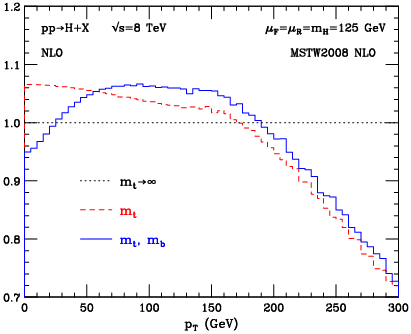
\includegraphics[width=0.5\textwidth]{images/pth_quarkmass.png}
\caption{\pth distribution computed at NLO ($\alpha_s^3$) and normalized to the calculation obtained in the large-$m_\mathrm{t}$ approximation. The red dashed line corresponds to the calculation including the top quark mass while the blue line refers to the calculation including also the bottom quark effects.}\label{fig:pth_quarkmass}
\end{figure}

Possible extensions of the SM predict a modification of the Higgs boson couplings to gluons and to the top quark. Many of these models actually predict the existence of new states that interact with the SM Higgs boson, but are beyond the direct production reach at the actual LHC energies. The effect of these new states could however show up as a deviation of the Higgs boson couplings with respect to the SM expectation. The modification of the couplings, as shown in Refs.~\cite{Azatov:2013xha,Harlander:2013oja}, can change the kinematics of the Higgs boson production and the effect can be particularly sizeable in the tail of the \pth distribution. 
Other models, such as Composite Higgs~\cite{Marzocca:2012zn}, predict the existence of top-partners, which are heavy resonances with the same quantum numbers as the top quark, that can interact with the Higgs boson in the ggH fermionic loop, changing the \pth shape with respect to what the SM predicts~\cite{Banfi:2013yoa}.
The measurement of the \pth spectrum is thus a useful tool for indirect searches of new particles predicted by theories beyond the SM.

Measurements of the fiducial cross sections and of several differential
distributions, using the $\sqrt{s}=8$\TeV LHC data, have been reported by ATLAS~\cite{Aad:2014tca,Aad:2014lwa,Aad:2015lha} and CMS~\cite{Khachatryan:2015rxa,Khachatryan:2015yvw} for the ${\mathrm{H} \to \mathrm{ZZ} \to 4\ell}$ ($\ell = \mathrm{e},\mu$) and H $\to \gamma\gamma$ decay channels. In this chapter a measurement of the fiducial cross section times branching fraction ($\sigma \times \mathcal{B}$) and \pt{} spectrum for Higgs boson production in \ensuremath{\mathrm{H}\rightarrow{}\WW\rightarrow \mathrm{e}^{\pm} \mu^{\mp}\nu\nu} ~decays, based on $\sqrt{s} = 8$\TeV LHC data, is reported.

The analysis is performed looking at different flavour leptons in the final state in order to suppress the sizeable contribution of backgrounds containing a same-flavour lepton pair originating from Z boson decay.

Although the \hwwllnn{} channel has lower resolution in the \pth{} measurement
compared to the H $\to \gamma\gamma$ and  H $\to \rm{ZZ}\to 4\ell$ channels
because of neutrinos in the final state, the channel has a significantly
larger $\sigma \times \mathcal{B}$, exceeding those for H $\to \gamma\gamma$ by a factor
of 10 and H $\to \rm{ZZ}\to 4\ell$ by a factor of 85 for a Higgs boson mass of
125\GeV~\cite{Heinemeyer:2013tqa}, and is characterized by good signal
sensitivity. Such sensitivity allowed the observation of a Higgs boson at the level of 4.3 (5.8 expected)
standard deviations for a mass hypothesis of 125.6 GeV using the full LHC data set at 7 and 8\TeV~\cite{Chatrchyan:2013iaa}.

The measurement is performed in a fiducial phase space defined by kinematic requirements on
the leptons that closely match the experimental event selection.

The effect of the limited detector resolution, as well as the
selection efficiency with respect to the fiducial phase space are corrected to
particle level with an unfolding procedure~\cite{Cowan:2002in}, as explained in Sec.~\ref{sec:Unfolding}.



%\clearpage
\section{Data sets and triggers}
%%%%%%%%%%%%%%%%%%%%%%%%%%%%%%%%%%%%%%%%%%%%%%%%%%%%%%%%%%%%%%%%%%%%%%
\label{sec:Datasets}

%-------------------------------------------------------------------------------
%\subsection{Data sets and triggers\label{subsec:Datasets}}
The data set used for this analysis corresponds to 19.4\ifb of proton-proton collisions at $\sqrt{s}=8$\TeV, collected by the CMS detector during 2012.
Only data corresponding to good data taking quality are considered.

Events are required to fire one of the unprescaled single-electron, single-muon or muon-electron triggers. Due the rather high LHC instantaneous luminosity the single-lepton triggers must have high HLT \pt thresholds, otherwise the rate of these triggers would be too large to be sustained. The double-lepton triggers allow to lower down the \pt thresholds while keeping a sustainable trigger rate, thus maintaining a good sensitivity to the Higgs boson signal, for which the lepton \pt can be rather small.
A brief overview of the HLT \pt criteria on the leptons
is given in Table~\ref{tab:trigger}. While the HLT lepton \pt thresholds of 17 and 8 \GeV for the double
lepton triggers accommodate the offline lepton \pt selection of 20 and 10 \GeV, the higher \pt thresholds
in the single lepton triggers help partially recovering double lepton trigger inefficiencies
as a high \pt lepton is on average expected due to the kinematic of the Higgs decay. 

\begin{table}[h]
\begin{center}
\caption{Transverse momentum thresholds applied in the lepton triggers at the HLT level. 
         Double set of thresholds indicates the thresholds for each leg of the double lepton triggers.}
\begin{tabular}{ccc}
\toprule
Trigger path       & Threshold \\
\midrule
Single electron    & $\pt > 27 $ \GeV         \\  
Single muon        & $\pt > 24 $ \GeV         \\ 
Muon-Electron      & $\pt > 17$ and $8 $ \GeV         \\ 
Electron-Muon      & $\pt > 17$ and $8 $ \GeV         \\ 
\bottomrule
\end{tabular}
\label{tab:trigger} 
\end{center}
\end{table}

The trigger is not simulated in MC samples but the combined trigger efficiency
is estimated from data and applied as a weight to all simulated events, as described in Sec.~\ref{sec:trigeff}.
% The trigger efficiency for single and double lepton triggers is calculated using a Tag and Probe technique separately for muons and electrons, in bins of $\eta$ and \pt.
%%%%%%%%%%%%%%%%%%%%
%%%%%%%%%%%%%%%%%%%% 

%SPOSTATO IN CAP. 2
%The Tag and Probe method uses a known mass resonance (e.g. $J/\Psi$, Z) to select particles of the desired type, and probe the efficiency of a particular selection criterion on these particles. In general the ``tag'' is an object that passes a set of very
%tight selection criteria designed to isolate the required particle type. Tags are often referred
%to as a “golden” electrons or muons and the fake rate for passing tag selection criteria should
%be very small. A generic set of the desired particle type (i.e. with potentially very loose selection criteria) known as ``probes'' is selected by pairing these objects with tags such that the
%invariant mass of the combination is consistent with the mass of the resonance. Combinatoric
%backgrounds may be eliminated through any of a variety of background subtraction methods
%such as fitting, or sideband subtraction. The definition of the probe objects depend on the
%specifics of the selection criterion being examined. The simple expression to get the efficiency $\epsilon$
%as a function of \pt and $\eta$ is given below:
%
%\begin{equation}
%\epsilon(\pt,\eta) = \frac{ N^\mathrm{probe}_\mathrm{pass}}{N^\mathrm{probe}_\mathrm{pass} + N^\mathrm{probe}_\mathrm{fail}}
%\end{equation}
%%%%%%%%%%%%%%%%%%%%%
%%%%%%%%%%%%%%%%%%%%%
%For double lepton triggers the efficiency is calculated separately for each leg of the trigger and then combined together. In the calculation the efficiencies of the two trigger legs are considered as independent, given that the correlations are very small. The combined efficiency is then used as a kinematics-dependent weight to be applied on top of simulated events.
%
%The event efficiency $\epsilon_\mathrm{ev}$ for an event with two leptons to pass the single lepton trigger is given by the following formula:
%
%\begin{equation}\label{eq:single_trigg}
%\epsilon_\mathrm{ev} = 1 - (1-\epsilon_{S,\ell1})\cdot(1-\epsilon_{S,\ell2})\quad,
%\end{equation}
%
%where $\epsilon_{S,\ell1}$ and $\epsilon_{S,\ell2}$ are the efficiencies for the leading and subleading lepton to pass the single lepton trigger. In other words, the dilepton event passes the single lepton trigger if either one of the two leptons passes the single lepton trigger, excluding the cases for which both leptons pass the trigger. For double lepton triggers, the event efficiency can be written as:
%
%\begin{equation}\label{eq:double_trigg}
%\epsilon_\mathrm{ev}  = \epsilon_{D,\ell1}^\mathrm{lead} \cdot \epsilon_{D,\ell2}^\mathrm{trail} + (  1 -  \epsilon_{D,\ell1}^\mathrm{lead} \cdot \epsilon_{D,\ell2}^\mathrm{trail})\cdot\epsilon_{D,\ell1}^\mathrm{trail} \cdot \epsilon_{D,\ell2}^\mathrm{lead} \quad,
%\end{equation}
%
%where $\epsilon_{D,\ell1}^{\mathrm{lead}(trail)}$ is the efficiency of the first lepton to pass the leading (trailing) leg of the double lepton trigger, and $\epsilon_{D,\ell2}^{\mathrm{lead}(trail)}$ is the efficiency of the second lepton to pass the leading (trailing) leg of the double lepton trigger. The final event efficiency applied to reweight the events in simulation is given by the boolean OR of the event efficiencies corresponding to the single and double lepton triggers, which, using Eqs.~\eqref{eq:single_trigg} and ~\eqref{eq:double_trigg}, can be written as:
%
%\begin{equation}
%\begin{split}
%\epsilon_\mathrm{ev} & = 1 - (1-\epsilon_{S,\ell1})\cdot(1-\epsilon_{S,\ell2}) + \\
%                     & + (1-\epsilon_{S,\ell1})\cdot(1-\epsilon_{S,\ell2}) \cdot \\
%                     & \cdot [ \epsilon_{D,\ell1}^\mathrm{lead} \cdot \epsilon_{D,\ell2}^\mathrm{trail} + (  1 -  \epsilon_{D,\ell1}^\mathrm{lead} \cdot \epsilon_{D,\ell2}^\mathrm{trail})\cdot\epsilon_{D,\ell1}^\mathrm{trail} \cdot \epsilon_{D,\ell2}^\mathrm{lead} ] \quad.
%\end{split}
%\end{equation}
%
%The term that multiplies the double lepton trigger event efficiency is needed to ensure that the events passing the double lepton trigger do not pass also the single lepton trigger.


%-------------------------------------------------------------------------------
\section{Monte Carlo samples\label{subsec:MC}}

Several Monte Carlo event generators are used to simulate the signal and background processes:
\begin{itemize}
\item the first version of the \textsc{Powheg} program (\textsc{Powheg V1}) provides event samples for the \hww signal
for the ggH and VBF production mechanisms, as well as \ttbar and tW processes~\cite{Alioli:2011as}, with NLO accuracy;
\item the VH process is simulated using \textsc{pythia 6.426}~\cite{Sjostrand:2006za};
\item the $\mathrm{qq} \to \mathrm{W^{+}W^{-}}$, Drell-Yan, ZZ, WZ, W$\gamma$, W$\gamma^*$, tri-bosons and W+jets processes are generated using
the \textsc{Madgraph 5.1.3} event generator;
\item the gg$\to \mathrm{W^{+}W^{-}}$ process is generated using the \textsc{gg2ww} 3.1 generator ~\cite{Binoth:2006mf} and its cross section is scaled to the approximate NLO prediction~\cite{Bonvini:2013jha,Passarino:2013bha}.
\end{itemize}
For samples generated at leading-order (LO) accuracy in perturbative QCD, the \textsc{cteq6l}~\cite{Lai:2010nw} set of parton distribution functions
(PDF) is used, while \textsc{ct10}~\cite{Lai:2010vv} is used for next-to-leading order (NLO) ones.
Cross section calculations at next-to-next-to-leading order (NNLO) are used for the \hww process~\cite{Dittmaier:2011ti}.
The $\hww$ process simulation is reweighted so that the \pth spectrum and inclusive production cross section closely match the SM calculations that have NNLO+NNLL QCD accuracy in the description of the Higgs boson inclusive production, in accordance with the LHC Higgs Cross Section Working Group recommendations~\cite{Heinemeyer:2013tqa}.
The reweighting of the \pth spectrum is achieved by tuning the \textsc{Powheg} generator, as described in detail in Ref.~\cite{Alioli:2010xd}.
Cross sections computed with NLO QCD accuracy are used for the background processes~\cite{Heinemeyer:2013tqa}.
The contribution of the \ttH production mechanism is checked to be negligible (below 1\%) in the whole \pth spectrum and is not included in the analysis. In Fig.~\ref{fig:signal_comp} the relative fraction of the four production mechanisms is shown for each \pth bin.

\begin{figure}[htb]
\centering
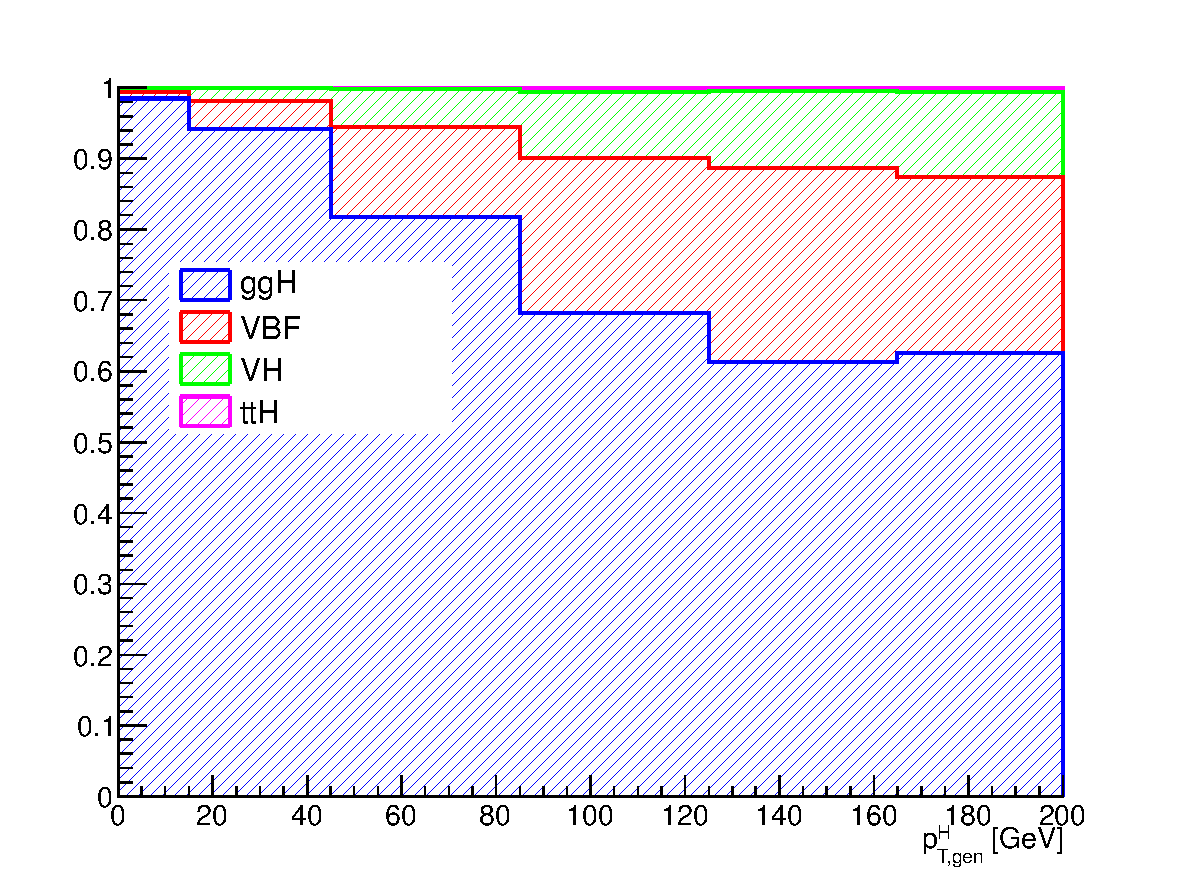
\includegraphics[width=0.7\textwidth]{images/signal_composition_ttH.pdf}
\caption{Relative fraction of ggH, VBF, VH and \ttH in each bin of the Higgs boson transverse momentum.}\label{fig:signal_comp}
\end{figure}

For all processes, the detector response is simulated using a detailed description of the CMS detector, based on the \textsc{Geant4} package~\cite{Agostinelli:2002hh}.

Minimum bias events are superimposed on the simulated events to emulate the additional 
proton-proton interactions per bunch crossing. The pile-up multiplicity in simulated events has been generated poissonianly sampling from a distribution similar to the one expected from data.
The simulated events are reweighted to correct for observed differences between data and simulation in the number of pile-up events, as shown in Fig.~\ref{fig:nvertices}.

\begin{figure}[htb]
\centering
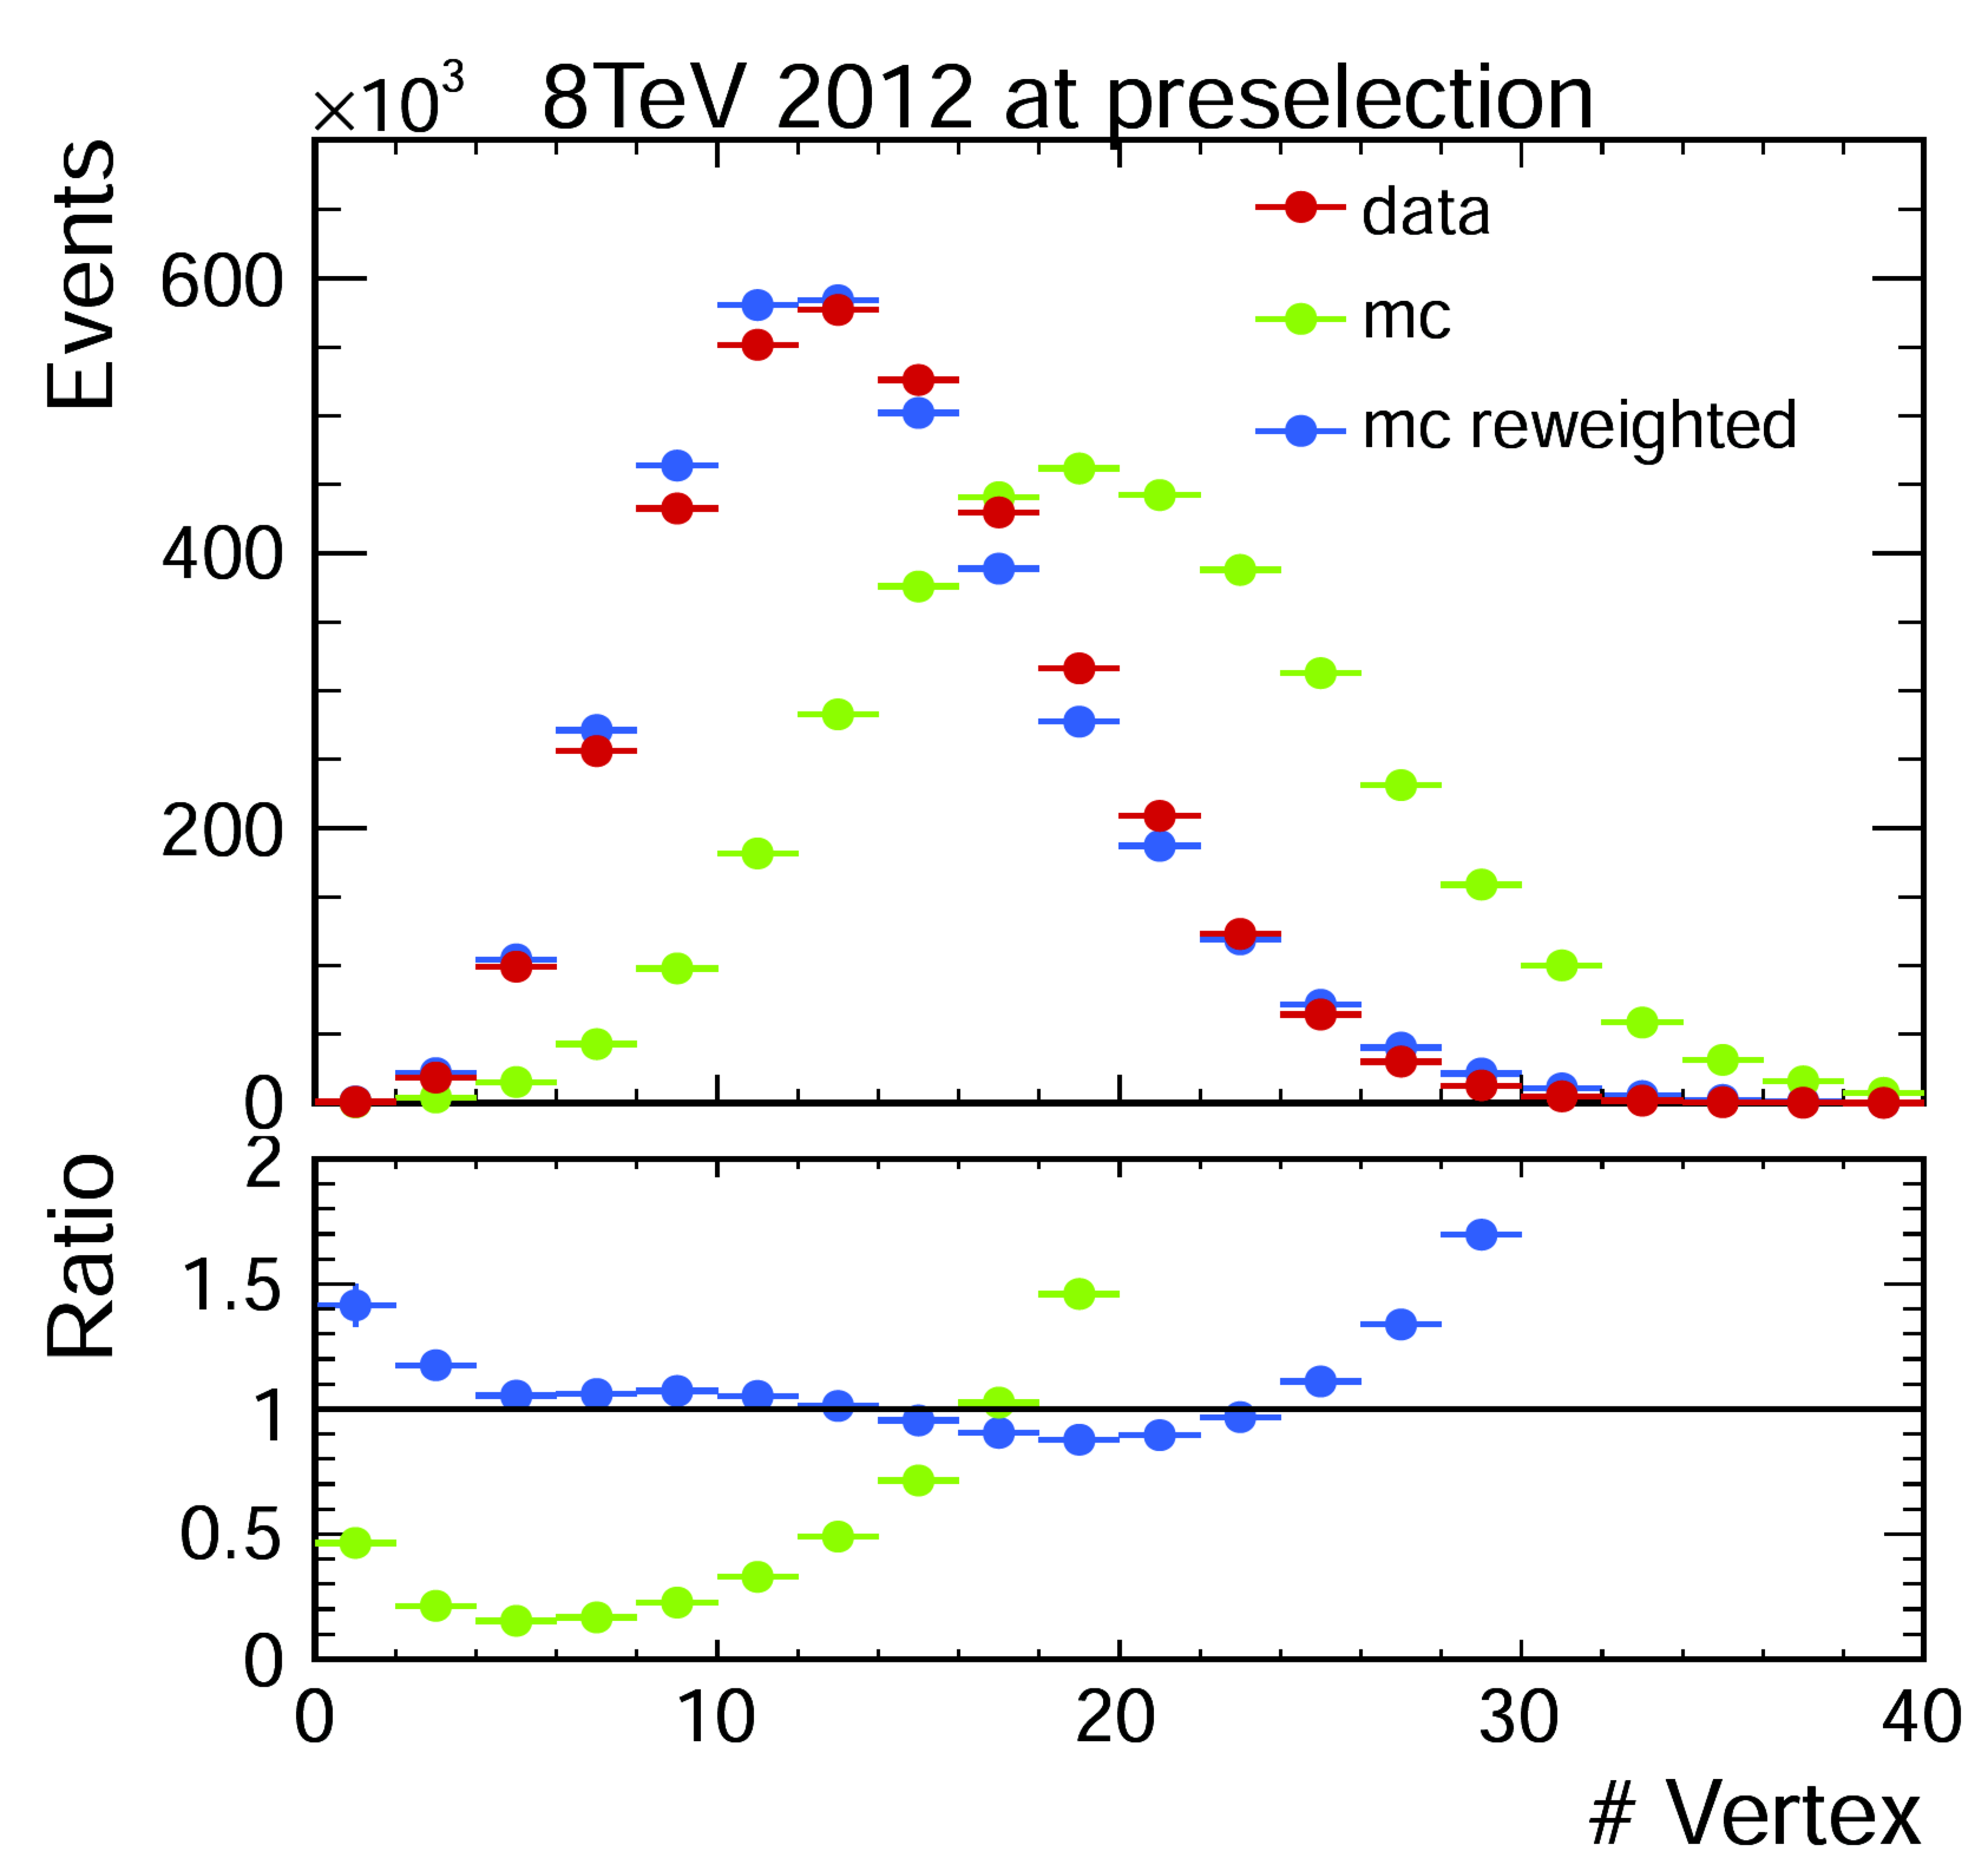
\includegraphics[width=0.7\textwidth]{images/nvertex.pdf}
\caption{Distribution of the number of vertices in data and simulation, before and after applying the pile-up reweighting.}\label{fig:nvertices}
\end{figure}

For the comparison of the measured unfolded spectrum with the theoretical predictions, two additional MC generators are used for simulating the SM Higgs boson production in the ggH process: \textsc{HRes} 2.3~\cite{deFlorian:2012mx,Grazzini:2013mca} and the second version of the \textsc{Powheg} generator (\textsc{Powheg V2})~\cite{Bagnaschi:2011tu}.
\textsc{HRes} is a partonic level MC generator that computes the SM Higgs
boson cross section at NNLO accuracy in QCD and performs the NNLL
resummation of soft-gluon effects at small \pt. The central predictions of
\textsc{HRes} are obtained including the top and bottom quark mass contribution to
the gluon fusion loop, fixing the renormalization and factorization scale central values at a Higgs boson mass of 125\GeV. The cross section normalization is scaled, to take into account electroweak corrections (by a factor of 1.05) and effects of threshold resummation (by a factor of 1.06)~\cite{Actis:2008ug,Catani:2003zt}. The upper and lower bounds of the uncertainties are obtained by scaling up and down both the renormalization and the factorization scales by a factor of two.
The \textsc{Powheg V2} generator is a matrix element based generator that provides a NLO description of the ggH process in association with zero jets, taking into account the finite mass of the bottom and top quarks.
The \textsc{Powheg} prediction is tuned using the \textsc{Powheg} damping factor \textit{hdump} of 104.17~\GeV, in order to match the \pth{} spectrum predicted by \textsc{HRes} in the full phase space. This factor reduces the emission of additional jets in the high \pt regime, and enhances the contribution from the Sudakov form factor in the limit of low \pt.
The \textsc{Powheg} generator is interfaced to the \textsc{JHUGen} generator version 5.2.5~\cite{Gao:2010qx,Bolognesi:2012mm,Anderson:2013afp} for the decay of the Higgs boson to a W boson pair and interfaced with \textsc{Pythia 8}~\cite{Sjostrand:2007gs} for the simulation of parton shower and hadronization effects.

%\clearpage
\section{Analysis Strategy}
%%%%%%%%%%%%%%%%%%%%%%%%%%%%%%%%%%%%%%%%%%%%%%%%%%%%%%%%%%%%%%%%%%%%%%
\label{sec:AnalysisStrategy}

The analysis presented here is based on that used in the previously published \hwwllnn{}
measurements by CMS~\cite{Chatrchyan:2013iaa}, modified to be inclusive in the number of jets. 
This modification significantly reduces the uncertainties related to the modelling of the number of jets produced in association with the Higgs boson.

The signal contribution is extracted performing a template binned likelihood fit, using the two-dimensional (\mll,\mt) shape for each background and signal process, as described in Sec.~\ref{sec:SignalExtraction}.

\textcolor{red}{controllare se mll e mT sono già stata definite}

\subsection{Event reconstruction and selections}\label{sec:Selections}

Electrons and muons used in the analysis are reconstructed using the PF technique as described in Sec.~\ref{sec:leptonID}. In particular, muon candidates are required to be identified both as Tracker Muons and Global Muons.

\begin{comment}
The electron selection is based on two multivariate discriminants, one specialised in identifying the electron object and the other for isolation. The cut value for each discriminant is optimised to provide a good fake electron rejection and to improve the signal acceptance.

Muons are reconstructed using the standard CMS selection and are required to be identified both in the tracker (\textit{Tracker Muon}) and in the muon chambers (\textit{Global Muon}). Additionally quality criteria on the muon track are required, such as to have at least 10 hits in the tracker (at least one of which in the pixel detector) and to have $\chi^2/ndf < 10$.
Muon isolation is based on the Particle-Flow algorithm. An MVA approach is considered, based on the radial distributions of the Particle-Flow candidates inside a cone of radius 0.5 around the muon direction.

The efficiencies for the identification and isolation of the electrons and muons are measured in data and in simulation selecting a pure sample of leptons coming from the Z$\to\ell\ell$ decay, and using a Tag and Probe technique very similar to the one described in Sec.~\ref{subsec:Datasets} for the trigger efficiency. In this case, the probe lepton is defined by loose isolation and identification requirements and the efficiency to pass the tight analysis selections is measured performing a simultaneous fit of signal plus background in two categories, corresponding to events in which the probe lepton pass or fail the analysis requirements. For the electrons, the resonant signal contribution in the fit is modelled as the convolution of a Breit-Wigner and a Crystal-Ball function. A polynomial function is added to take into account the tail in the low mass region. For muons the signal is fitted using the sum of two Voigtian functions. For both electrons and muons the background contribution is modelled as a third order Bernstein polynomial function.
The efficiencies for data and simulation are extracted as parameters of the fit and are used as scale factors to correct the MC simulation to precisely model the data.
\end{comment}

Jets are reconstructed using the standard PF algorithm and using the anti-$k_t$ clustering algorithm with $\mathrm{R} = 0.5$, as described in Sec.~\ref{sec:jets}. If not specified otherwise, jets considered for jet counting are the ones with $\pt > 30$\,\GeV.

In addition to the standard CMS PF \MET, in this analysis a \textit{projected} \MET variable is also used. The \textit{projected} \MET is defined as the component of \ptmiss transverse to the nearest lepton if the lepton is situated within the azimuthal angular window of $\pm \pi/2$ from the \ptmiss direction, or the \MET itself otherwise.
Since the \MET resolution is degraded by pileup, the minimum of two projected \MET variables is used: one constructed from all identified particles (full projected \MET), and another constructed from the charged particles only (track projected \MET).

Background events from \ttbar and tW production are rejected applying a soft-muon veto and b tagging veto. The soft-muon algorithm is designed to identify muons from b quark decays. Events containing a muon satisfying the following requirements are rejected by the soft-muon veto: 
\begin{itemize}
\item reconstructed as TrackerMuon;
\item number of hits in the Silicon Tracker greater than 10;
\item transverse impact parameter less than 0.2\,cm;
\item relative isolation greater than 0.1 for muons with $\pt>20$\,\GeV.
\end{itemize}

The b tagging veto rejects events that contain jets identified as b-jets using two different algorithms for high and low \pt jets (see Sec.~\ref{sec:btag}). For jets with \pt between 10 and 30\GeV, the TCHE algorithm is applied. Low-\pt jets passing the TCHE discriminant threshold of 2.1 are tagged as b-jets.
For jets with $\pt>30$\GeV, a better performing algorithm, JP, is used. Jets are identified as b-jets by the JP algorithm if the discriminating variable has a value above 1.4.
In the following, a b tagged jet is defined as a jet, within $|\eta|<2.4$ (b-tagging requires the tracker information), and with a value of the discriminating variable above the mentioned thresholds for the two algorithms.


%%% Event selection
The event selection consists of several steps. The first step is to select \WW-like events applying a selection that consists of the following set of cuts:
\begin{enumerate}
\item {\bf Lepton preselection}:
  \begin{itemize}
  \item two opposite charge and different flavour (e$\mu$) isolated leptons reconstructed in the event;
  \item $|\eta|<2.5$ for electrons and $|\eta|<2.4$ for muons;
  \item $\pt>20\GeV$ for the leading lepton. For the trailing lepton, the transverse momentum is required to be larger than 10\GeV.
  \end{itemize}
\item {\bf Extra lepton veto}: the event is required to have two and only two leptons with opposite charge passing the lepton selection.
\item {\bf \MET preselection}: particle flow \MET is required to be greater than 20\GeV.
\item {\bf projected \MET selection}: minimum projected \MET required to be larger than 20\GeV.
\item {\bf Di-lepton mass cut}: $\mll > 12$\GeV in order to reject low mass resonances and QCD backgrounds.
\item {\bf Di-lepton \pt cut}: $\ptll > 30$\GeV to reduce the contribution of W+jets and DY to $\tau\tau$ backgrounds.
\item {\bf Transverse mass}: $\mt>60$\GeV to reject DY to $\tau\tau$ events. 
\end{enumerate}
The requirement of different flavour leptons in the final state is important in order to suppress the sizeable contribution of backgrounds containing a same flavour lepton pair originating from Z boson decay.

Events surviving these requirements are dominantly those where a top quark-antiquark pair is produced and both W bosons, which are part of the top quark decay chain, decay leptonically (dileptonic \ttbar).
Two different selections are used depending on the number of jets in the event. This is done to suppress the top quark background both in the low \pth region, where 0-jets events have the largest contribution, and for higher \pth values where also larger jet multiplicity events are important.
The selection for 0-jets events relies on the soft-muon veto and on a soft jet (with $\pt < 30$\GeV) b tagging veto.
The latter requirement exploits the TCHE algorithm to reject soft jets that are likely to come from b quarks hadronization.

For events with a jet multiplicity greater or equal than one, a different selection is applied. In this case we exploit the good b tagging performances of the JP tagger to reject all the jets with $\pt > 30$\GeV that are likely to come from b quarks hadronization. The analysis selection requires to have no events containing b-tagged jets with $\pt > 30$\GeV.

\begin{figure}[htb]
\centering
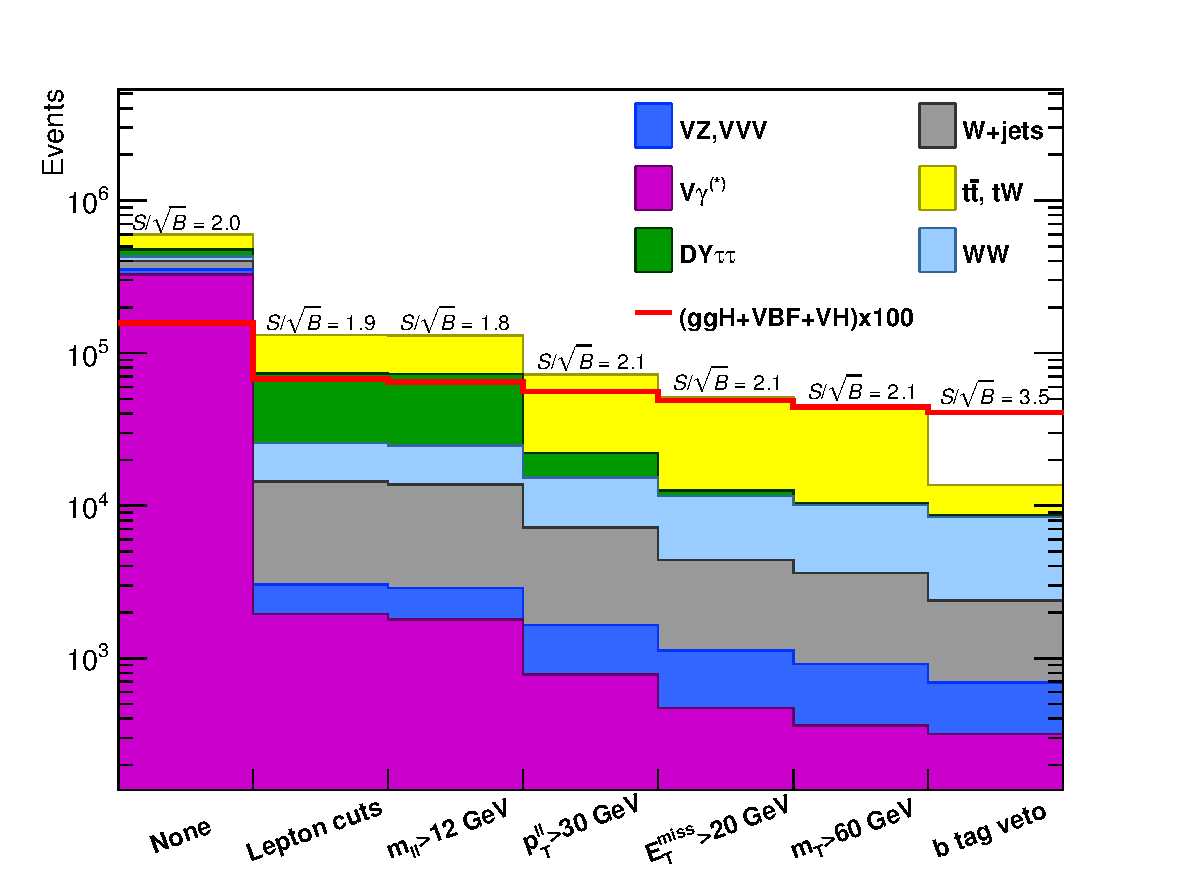
\includegraphics[width=0.8\textwidth]{images/cutflow-thesis.pdf}
\caption{Effect of selection cuts on simulated samples. The signal (red line) is multiplied by 100 and superimposed on stacked backgrounds. In each bin, corresponding to a different selection, is reported the expected number of events in MC at a luminosity of $19.46~\mathrm{fb}^{-1}$.}\label{fig:cutflow}
\end{figure}

A cut-flow plot is reported in Fig.~\ref{fig:cutflow}, showing the effect of each selection using signal and background simulations. In the first bin, labelled as ``No cut'', no selection is applied and the bin content corresponds to the total expected number of events with a luminosity of $19.4~\mathrm{fb}^{-1}$. All the events in this bin have at least two leptons with a loose transverse momentum cut of 8\GeV. In the following bin the lepton cuts are applied, including the requirement to have two opposite sign and different flavour leptons and the extra lepton veto. Then all the other selections are progressively reported, showing the effect of each cut on the background and signal yields. For each selection the expected signal over background ratio is also shown, which, after the full selection requirements, reaches a maximum value of about $3\%$.




\subsection{Simulation efficiencies and scale factors}\label{sec:ScaleFactors}

The efficiencies for the identification and isolation of the electrons and muons are measured in data and simulation selecting a pure sample of leptons coming from the Z$\to\ell\ell$ decay, and using the Tag and Probe technique described in Sec.~\ref{sec:lepIdIsoEff}. The efficiencies for data and simulation are used as scale factors to correct the simulated events to precisely model the data.

The trigger efficiency is measured in data and applied to simulation as explained in Sec.~\ref{sec:trigeff}.

The efficiency of b tagging algorithms is not well simulated by MC generators and discrepancies can occur with respect to the data. For this reason is important to measure the b tagging efficiency and the misidentification probability for the given algorithms both in data and simulation, and to correct the simulated events using scale factors. This affects not only the top quark background estimation, but also the other backgrounds and the signal. As an example, if a light-parton jet in a signal event was misidentified as a b-jet, this event would be rejected by the b-jet veto.

In this analysis, the b tagging efficiency and the misidentification probability are measured both in data and simulation, selecting a control sample enriched in b-jets, and using a Tag and Probe technique similar to the one described in Sec.~\ref{sec:lepIdIsoEff}. Below is described the method used to estimate the efficiency of the JP b tagging algorithm, but it is extendible to any other algorithm.

The control sample is defined selecting the events that pass the selections listed in Sec.~\ref{sec:Selections}, and have at least two jets with \pt greater than 30 \GeV. If the leading jet has a JP discriminator values above the threshold of 0.5, it is considered a \emph{tag}, and the sub-leading jet is the \emph{probe}. In order to avoid any bias that could arise from the probe being always the sub-leading jet, the pair is tested also in reverse order, i.e. sub-leading jet is tested against the \emph{tag} selection, and in case it passes, then the leading jet is used as \emph{probe} forming an independent \emph{tag-probe} pair. If the \probe jet has a discriminator value above the threshold used in the analysis, i.e. $>1.4$, then the \tp pair is called a \tpp pair. Otherwise it is identified as a \tfp pair.

If the \tg selection was sufficient to suppress any non top quark event, one could estimate the efficiency by dividing the number of \tp pairs in which the \probe passes the analysis JP requirement by the total number of \tp pairs. However this is not the case, since the contamination due to other background sources is not negligible. In order to estimate the efficiency in the presence of background, a variable that discriminates between true b-jets and other jets in a \ttbar sample is needed. This variable is the \pt of the \probe jet. For real b-jets this variable has a peak around 60\GeV, while it has a broad distribution for other types of jets.

The efficiencies are estimated performing a $\chi^{2}$ simultaneous fit of the \probe \pt spectrum in two different categories: one containing events with a \tpp pair and the other containing events with a \tfp pair. The normalisations in the two categories are linked by the following formulas:

\begin{equation}
\begin{split}
N_\mathrm{TPP} &= N_\mathrm{s} \varepsilon_\mathrm{s} + N_\mathrm{b} \varepsilon_\mathrm{b} \\
N_\mathrm{TFP} &= N_\mathrm{s} (1 -\varepsilon_\mathrm{s}) + N_\mathrm{b} ( 1 - \varepsilon_\mathrm{b}) \quad,
\end{split}
\end{equation}

where:
\begin{itemize}
\item $N_\mathrm{TPP}$ is the number of \tpp pairs;
\item $N_\mathrm{TFP}$ is the number of \tfp pairs;
\item $N_\mathrm{s}$ is the number of \tp pairs in which the \probe is a b-jet;
\item $N_\mathrm{b}$ is the number of \tp pairs in which the \probe is not a b-jet;
\item $\varepsilon_\mathrm{s}$ is the efficiency to identify a b-jet, i.e. the b tagging efficiency;
\item $\varepsilon_\mathrm{b}$ is the probability to misidentify a non b-jet as a b-jet, i.e. the misidentification probability\footnote{In these naming convention, the subscript ``s'' stays for ``signal'', since the b-jets represent the signal in this method. Similarly, the ``b'' subscript stays for ``background'', identifying the cases where the \probe is not a b-jet}.
\end{itemize}

The \pt shapes of the \probe jet used in the fit are taken from simulation, where the real flavour of the jet is known, both for the \tpp and \tfp categories. To check the consistency of the fitting procedure, a closure test fitting the simulation itself has been performed.
The result of the fit on MC simulation is shown in Fig.~\ref{fig:mc_tp}. The relevant efficiencies are:
\begin{equation}
\begin{split}
\varepsilon_\mathrm{s}^\mathrm{MC} &= 0.766\pm0.007 \\
\varepsilon_\mathrm{b}^\mathrm{MC} &= 0.208\pm0.015 \quad .
\end{split}
\end{equation}
These values are consistent with the true value of the b tagging efficiency in simulation. The true value is computed by selecting jets that are matched within a cone of $\Delta{R}<0.5$ with a generator level b quark, and counting the fraction of those that have a JP discriminator above threshold of 1.4. This check also assures that the \tp method does not introduce any bias within the simulation statistic accuracy.

\begin{figure}[htb]
\centering
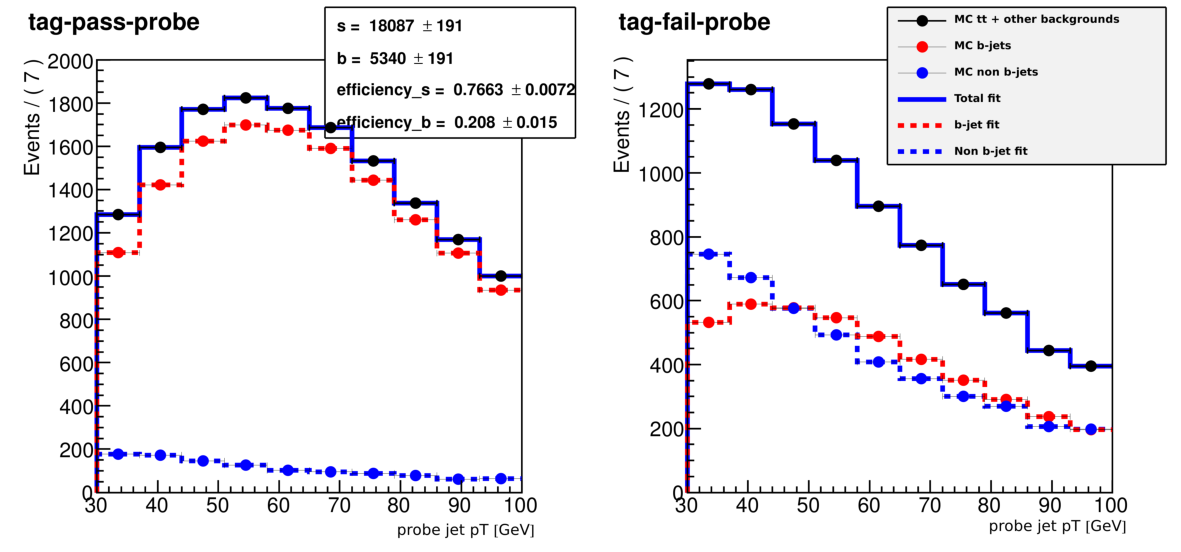
\includegraphics[width=0.8\textwidth]{images/mc_pt_probe-v2.pdf}
\caption{Simultaneous fit of the \tpp and \tfp pairs in the MC.\label{fig:mc_tp}}
\end{figure}

In order to assess the robustness of the fit, 5000 toy simulated samples have been generated with a statistics equivalent to the one expected in data and the same fit is performed. All the 5000 fit succeeded, and the pull distributions for $\varepsilon_{\rm s}$ and $\varepsilon_{\rm b}$ parameters are shown in Fig.~\ref{fig:pullstp}. The distributions represent the \emph{pull} of the efficiencies measured in the fit, where the pull variable for each toy $i$ is defined as:

\begin{equation}
pull(\varepsilon_{\rm s (b)}) = \frac{\varepsilon_{\rm s (b)}^{\rm true} - \varepsilon_{\rm s (b)}^{i}}{\sigma(\varepsilon_{\rm s (b)}^{i})} \quad,
\end{equation}

where $\sigma(\varepsilon_{\rm s (b)}^{i})$ is the uncertainty on the efficiency extracted from the fit. The pull distributions are centred on zero and have $\sigma$ close to one, as expected.

Before running the fit on data, the shapes used in the fit have been validated. To do so, a very pure phase space enriched in b jets has been defined by selecting events containing exactly two jets with a JP discriminator greater than 1.5 and no additional b-tagged jets, rejecting also events containing jets with \pt smaller than 30 \GeV. On this very pure sample, data have been compared against the shape used to fit the true b-jets in the \tpp distribution. The result is shown in Fig.~\ref{fig:purett} and shows good agreement within uncertainties.

\begin{figure}[htb]
\centering
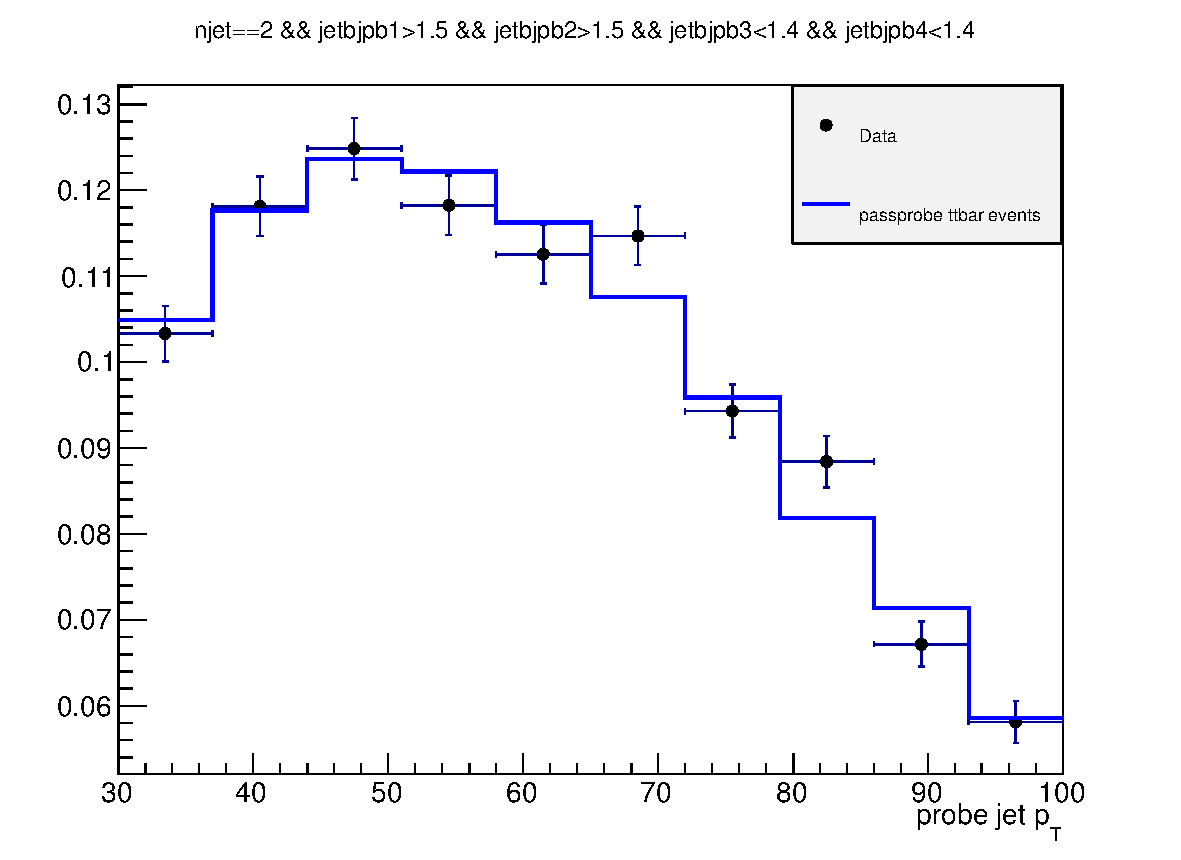
\includegraphics[width=0.6\textwidth]{images/passprobe_data_mc.pdf}
\caption{Shape comparison for the \pt spectrum of the \probe jet in data and simulation in a very pure phase space enriched in b-jets.\label{fig:purett}}
\end{figure}

Finally the fit has been performed on data, as shown in Fig.~\ref{fig:data_tp}, providing the following efficiencies:

\begin{equation}
\begin{split}
\varepsilon_\mathrm{s}^\mathrm{Data} &= 0.77\pm0.02\\
\varepsilon_\mathrm{b}^\mathrm{Data} &= 0.12\pm0.05
\end{split}
\end{equation}

\begin{figure}[htb]
\centering
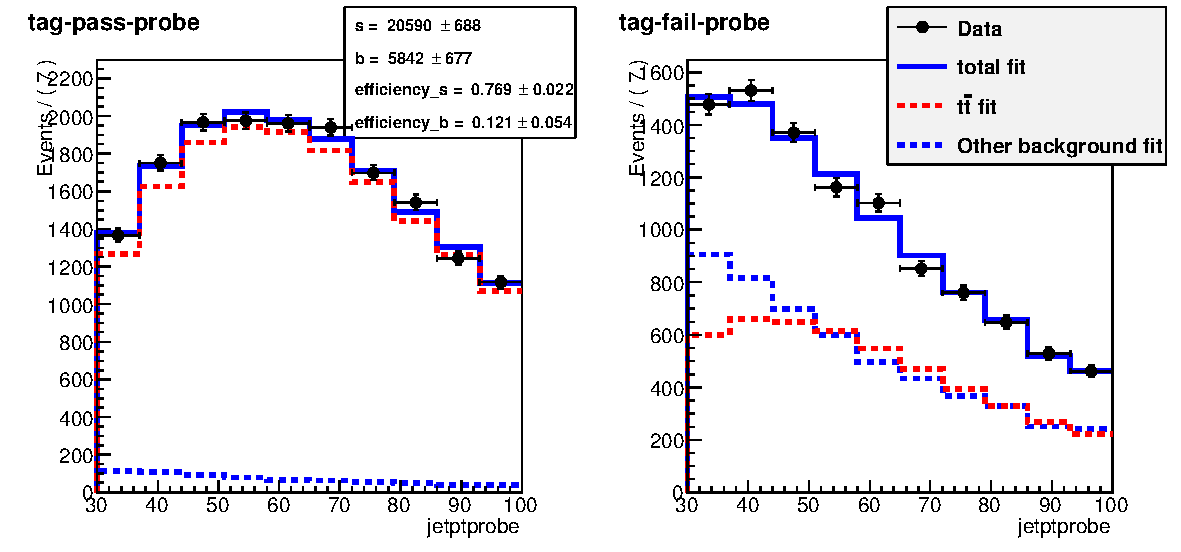
\includegraphics[width=0.8\textwidth]{images/data_ptprobe.pdf}
\caption{Simultaneous fit of the \tpp and \tfp pairs in data.\label{fig:data_tp}}
\end{figure}

Further studies have been performed to assess the effect of the relative uncertainty on the \ttbar and tW event fractions. The same procedure described above has been applied to different simulation templates obtained varying the \ttbar and tW fractions within theoretical uncertainties, and the effect on the parameters extracted with the fit procedure is found to be well below the fit uncertainties.

The ratio of the efficiency measured in data and simulation represents a per-jet scale factor that can be used to reweight the simulated events. The weights to be applied event-by-event depend on the particular jet configuration in the events itself. For the signal region ($SR$), in which a b tagging veto is required, the event weight to be applied is given by:

\begin{equation}
w_{SR} = \prod_{N_\mathrm{b-jets}} \left( \frac{1-\varepsilon_\mathrm{s}^\mathrm{Data}}{1-\varepsilon_\mathrm{s}^\mathrm{MC}} \right) \prod_{N_\mathrm{non~b-jets}} \left( \frac{1-\varepsilon_\mathrm{b}^\mathrm{Data}}{1-\varepsilon_\mathrm{b}^\mathrm{MC}} \right) \quad ,
\end{equation}

where $N_\mathrm{b-jets}$ and $N_\mathrm{non~b-jets}$ are the number of true b-jets and the number of non b-jets in the simulated event, respectively. This weight is valid if the a b tagging veto is applied. If instead the b tagging veto is reverted, also the event weight has to be modified. This is done, for example, when one wants to define a \ttbar enriched control region ($CR_{\ttbar}$) for the purpose of measuring the contribution of this background in a phase space orthogonal to the signal region. One simple way to define this control region is to require the leading jet in the event to be b-tagged. Therefore, the simulated events falling in this category must be reweighted using the following weight:

\begin{equation}
w_{CR_{\ttbar}} = 
\begin{cases}
\varepsilon_\mathrm{s}^\mathrm{Data}/\varepsilon_\mathrm{s}^\mathrm{MC},& \text{if the leading jet is a b-jet} \\
\varepsilon_\mathrm{b}^\mathrm{Data}/\varepsilon_\mathrm{b}^\mathrm{MC},& \text{if the leading jet is not a b-jet} 
\end{cases}
\end{equation}




\subsection{Fiducial phase space}\label{sec:fid_space}
The Higgs boson transverse momentum is measured in a fiducial phase space, whose definition is chosen in order to minimize the dependence of the measurements on the underlying model of the Higgs boson production and decay properties.

The exact requirements are determined by considering the two following correlated quantities: the reconstruction efficiency for signal events originating from within the fiducial phase space (fiducial signal efficiency $\varepsilon_{\rm{fid}}$), and the ratio of the number of reconstructed signal events that are from outside the fiducial phase space (``out-of-fiducial'' signal events) to the number from within the fiducial phase space. The requirement of having a small fraction of out-of-fiducial signal events, while at the same time preserving a high value of the fiducial signal efficiency $\epsilon_{\rm{fid}}$, leads to fiducial requirements at the generator level on the low-resolution variables, \MET and \mt, that are looser with respect to those applied in the reconstructed event selection.

The fiducial phase space used for the cross section measurements is defined at the particle level by the requirements given in Table~\ref{table:fid_cuts}. The leptons are defined as Born-level leptons, i.e. before the emission of final-state radiation (FSR), and are required not to  originate from leptonic $\tau$ decays. The effect of including FSR is found to modify $\epsilon_{\rm{fid}}$ at most of about 5\%.
For the VH signal process, the two leptons are required to originate from the \hwwllnn decays in order to avoid including leptons coming from the associated W or Z boson.

\begin{table}[htb]
\caption{Summary of requirements used in the definition of the fiducial phase space.}\label{table:fid_cuts}
\begin{center}
\begin{tabular}{l r}\hline\hline
\bf{Physics quantity} & \bf{Requirement} \\
\hline
Leading lepton \pt & $\pt > 20$\GeV \\
Subleading lepton \pt & $\pt > 10$\GeV \\
Pseudorapidity of electrons and muons & $|\eta| < 2.5$ \\
Invariant mass of the two charged leptons & $\mll > 12$\GeV \\
Charged lepton pair \pt & $p_{\rm T}^{\ell\ell} > 30$\GeV \\
Invariant mass of the leptonic system in the transverse plane & $m_{\rm T}^{\ell\ell \nu\nu} > 50$\GeV \\
\MET & $\MET>0$ \\
\hline
\end{tabular}
\end{center}
\end{table}

A detailed description of the fiducial region definition and its optimization is given in appendix \ref{app:fiducial_region}.










\subsection{Binning of the \pth distribution}

Experimentally, the Higgs boson transverse momentum is reconstructed as the vector sum of the lepton momenta in the transverse plane and \MET.
\begin{equation}
\vec{p}_\mathrm{T}^\mathrm{~H} = \vec{p}_\mathrm{T}^{~\ell\ell} + \vec{p}_\mathrm{T}^\mathrm{~miss}
\end{equation}
Compared to other differential analyses of the Higgs cross section, such as those in the ZZ and $\gamma\gamma$ decay channels, this analysis has to cope with the limited resolution due to the \MET entering the transverse momentum measurement.
The effect of the limited \MET resolution has two main implications on the analysis strategy: the first one is that the choice of the binning in the \pth{} spectrum needs to take into account the detector resolution; the second implication is that migrations of events across bins are significant and an unfolding procedure needs to be applied to correct for selection efficiencies and bin migration effects.

Given these aspects, the criterion that is used to define the \pth bin size is devised to keep under control the bin migrations due to the finite resolution.
For any given bin $i$, the purity $P_i$ of the signal sample is defined as the number events that are generated and also reconstructed in that bin, i.e. $N_i^\mathrm{GEN|RECO}$, divided by the number of events reconstructed in the same bin, $N_i^\mathrm{RECO}$:

\begin{equation}
P_i = \frac{N_i^\mathrm{GEN|RECO}}{N_i^\mathrm{RECO}} \quad .
\end{equation}

The bin width is chosen in such a way as to make the smallest bins able to ensure a purity of about 60\%, based on a ggH simulated sample.
Following this prescription, the whole \pth range is dividedin the following six bins: \mbox{[0--15]\GeV}, \mbox{[15--45]\GeV}, \mbox{[45--85]\GeV}, \mbox{[85--125]\GeV}, \mbox{[125--165]\GeV}, \mbox{[165--$\infty$]\GeV}.

The fiducial signal efficiency $\varepsilon_\mathrm{fid}$ and the fraction of out-of-fiducial signal events, $f_\mathrm{out-of-fid}$, are different in each \pth bin and depend on the definition of the fiducial phase space. In Fig.~\ref{fig:sel_eff} the $\varepsilon_\mathrm{fid}$ and $f_\mathrm{out-of-fid}$ parameters are shown in each \pth bin for different definitions of the fiducial phase space. In particular, they have been evaluated adding the requirements reported in Table~\ref{table:fid_cuts} in sequence, starting from a fiducial phase space defined just by the lepton \pt and $\eta$ selections, together with the different flavour requirement, and adding each time an additional selection until the full fiducial phase space in obtained. In this way, the effect of every single selection (or group of selections) on $\varepsilon_\mathrm{fid}$ and $f_\mathrm{out-of-fid}$ can be assessed. Since the variables related to leptons are measured with good resolution, the effect of including the related selections in the fiducial phase space is to increase $\varepsilon_\mathrm{fid}$ keeping $f_\mathrm{out-of-fid}$ constant. Instead, the effect of including low-resolution variables, such ad \mt, is to increase both $\varepsilon_\mathrm{fid}$ and $f_\mathrm{out-of-fid}$. Nevertheless, the $f_\mathrm{out-of-fid}$ parameter is different from zero even if only lepton cuts are taken into account. This is ascribable to two different aspects: the first one is that in the fiducial definition electrons and muons are required not to originate from $\tau$ decays; the second one is instead related to the VH production mechanism, i.e. to the fact that leptons coming from the associated boson are not included.

%The efficiency of the analysis selection with respect to the fiducial phase space is reported in Fig.~\ref{fig:sel_eff} (a) for each \pth bin. The efficiency denominator is the number of events that are inside the fiducial phase space, while the numerator is the number of events that pass both the analysis and the fiducial phase space selections. The fake rate, defined by the ratio of signal events that pass the analysis selection but are not within the fiducial phase space, divided by the total number of events passing both the analysis and the fiducial phase space selections is shown in Fig.~\ref{fig:sel_eff} (b). For both the selection efficiency and the fake rate, all the signal production mechanisms are included.
The overall values integrating over \pth are $\varepsilon_\mathrm{fid}=0.362\pm{0.005}$ and $f_\mathrm{out-of-fid}=0.126\pm0.004$ respectively, where only statistical uncertainties are taken into account.

\begin{figure}[htb]
\centering
\subfigure[]{
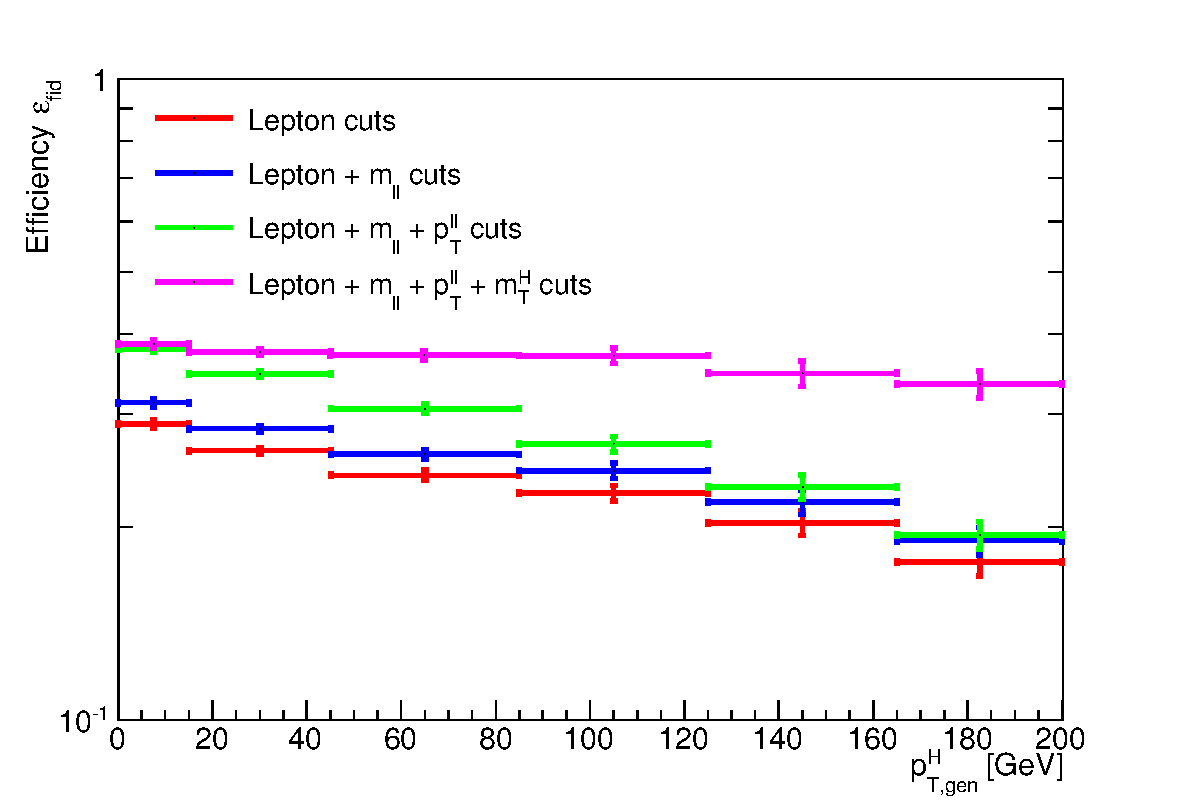
\includegraphics[width=0.45\textwidth]{images/eff-fid.pdf}
}
\subfigure[]{
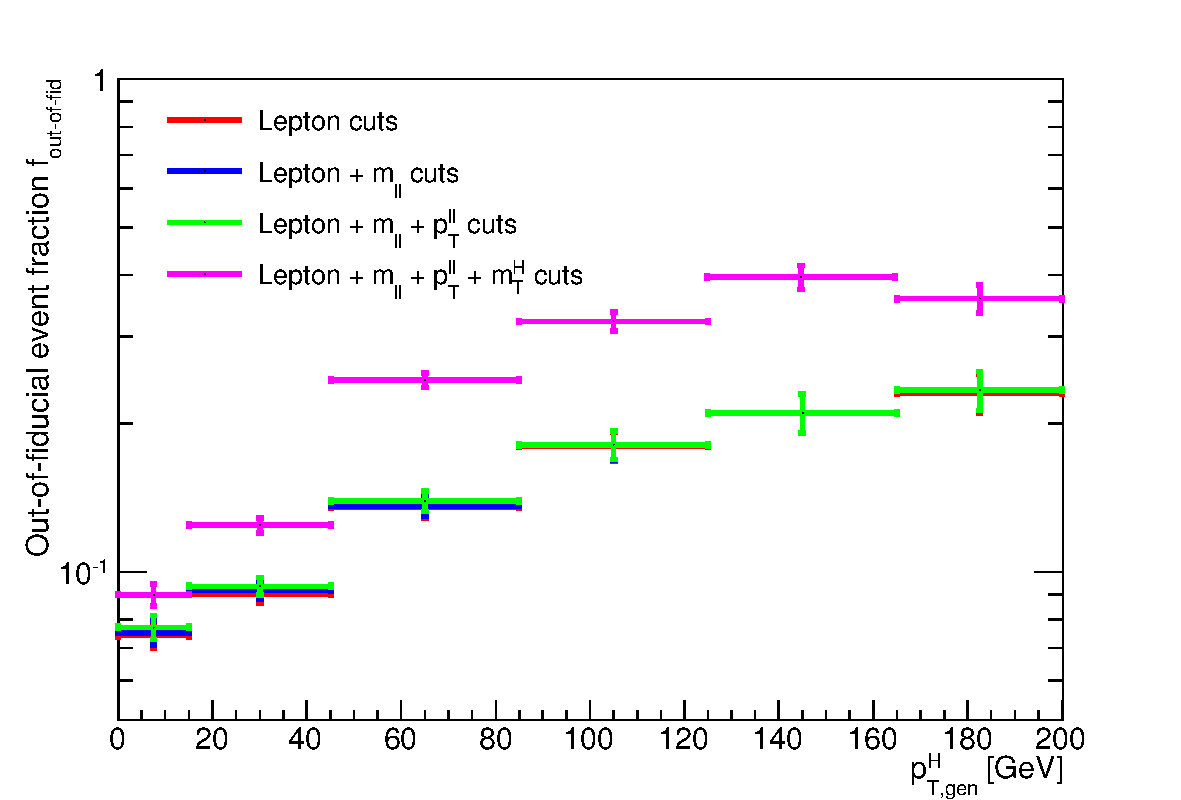
\includegraphics[width=0.45\textwidth]{images/out-of-fid.pdf}
}
\caption{Fiducial signal efficiency $\varepsilon_\mathrm{fid}$ and fraction of out-of-fiducial signal events $f_\mathrm{out-of-fid}$ in each bin of the generator level \pth.\label{fig:sel_eff}}
\end{figure}

If a $4\pi$ acceptance is defined, requiring just that the Higgs decays to WW and then to $2\ell2\nu$, the efficiency becomes $\epsilon=0.0396\pm{0.0003}$ and the fake rate is zero. 






%\clearpage
%%-------------------------------------------------------------------------------
\section{Event reconstruction and selections\label{sec:Selections}}

	%--------------------------------------------------------------------------------
	\subsection{Event reconstruction\label{subsec:EventReconstruction}}
The muons, electrons, jets and missing transverse energy (\MET) reconstruction and criteria are described in
in details in~\cite{AN-2012-194}. The following criteria are only a brief summary:
\begin{itemize}
\item {\bf Muons:} {\it GlobalMuon} 
                   (with $\chi^2/ndof < 10$, at least one good muon hit and at least two muon segments in different muon stations)  
                   or {\it TrackerMuon}  (provided it satisfies the "Tracker Muon Last Station Tight" selection). Several cut-based identification 
                   criteria are applied as well as the particle flow (PF) Isolation. In 2012, the PF Isolation is replaced
                   by an MVA algorithm.
\item {\bf Electrons:} {\it GSF Electons}. A MVA identification criteria is applied  as well as an MVA algorithm.
\item {\bf Jets:}  {\it Anti-$k_T$ PF jets} (with R=0.5 and applying L1, L2 and L3 jet energy corrections, including Pile-Up jet corrections from Fastjet method). Only jets and $|\eta|<4.7$ are considered. A specific Pile-Up MVA-based rejection algorithm is applied.   
\item {\bf \MET:}  The \MET is reconstructed the {\it PF Algorithm} or considering {\it only tracks} originating from the same vertex as 
                   the two leptons. In addition, the minimum of the projections of these two \MET to the closest lepton direction if they are in the same hemisphere, otherwise of their original values, is used in the analysis.  
\end{itemize}

	%--------------------------------------------------------------------------------
	\subsection{Event selection\label{subsec:EventSelection}}
Unlike the main \hwwllnn analysis, this analysis is inclusive in number of jets, so we do not have to define different jet multiplicity categories.
The event selection consist of several steps. The first step is to select \WW -like events applying a selection that is heavily based on the main analysis selection except for few different cuts explained below.
The \WW -like event preselection consists of the following set of cuts:
\begin{enumerate}
\item {\bf Lepton preselection}:
  \begin{itemize}
  \item at least two opposite-sign and opposite-flavour ($e\mu$) leptons reconstructed in the event;
  \item $|\eta|<2.5$ for electrons and $|\eta|<2.4$ for muons;
  \item $\pt>20~\GeV$ for the leading lepton. For the trailing lepton, the transverse momentum is required to be larger than 10~\GeV.
  \end{itemize}
\item {\bf Extra lepton veto}: the event is required to have two and only two opposite-sign leptons passing the lepton selection.
\item {\bf \MET preselection}: particle flow \MET is required to be greater than $20$\GeV.
\item {\bf Di-lepton mass cut}: $m_{\ell\ell} > 12$\GeV in order to reject low mass resonances and QCD backgrounds.
\item {\bf Di-lepton $p_T$ cut}: $p_T^{\ell\ell} > 30$\GeV.
\item {\bf projected \MET selection}: minimum projected \MET required to be larger than 20~\GeV.
\item {\bf Transverse mass}: $m_T^H>60$\GeV to reject Drell-Yan to $\tau\tau$ events. 
\end{enumerate}
In addition to the \WW-like preselection other cuts are applied in order to reduce the top background (\ttbar ans single-top), which is one of the main backgrounds in this final state. We operate two different selections depending on the number of jets with $p_T > 30$~\GeV in the event. This is done to suppress the top background both in the low $p_T^H$ region, where 0-jets events have the biggest contribution, and for higher values where also larger jet multiplicity events are important.
The selection for 0-jets events relies on a soft muon veto, which rejects events with non-isolated soft muons (likely belonging to b-jets), and on a soft jets (with $p_T < 30$~\GeV) anti b-tagging requirement.
The latter requirement exploits the Track Counting High Efficiency tagger (TCHE) to reject soft jets that are likely to come from b quarks hadronization.
These are exactly the same requirements applied in the 0-jets bin of the main analysis.

For events with a jet multiplicity greater or equal than one, we apply a different selection with respect to the main analysis. In this case we exploit the good b-tagging performances of the \textit{JetBProbability} tagger to reject all the jets with $p_T > 30$~\GeV that are likely to come from a b quark. This jet veto relies on a cut on the \textit{JetBProbability} tagger discriminant as has been also done in the VH (\hwwllnn) analysis \cite{CMS_PAS_HIG_13-017}. Any jet with a discriminant value below $1.4$ is identified as a non b-jet. The analysis selection requires no b-tagged jets with $p_T > 30$~\GeV.

\begin{figure}[b]
\centering
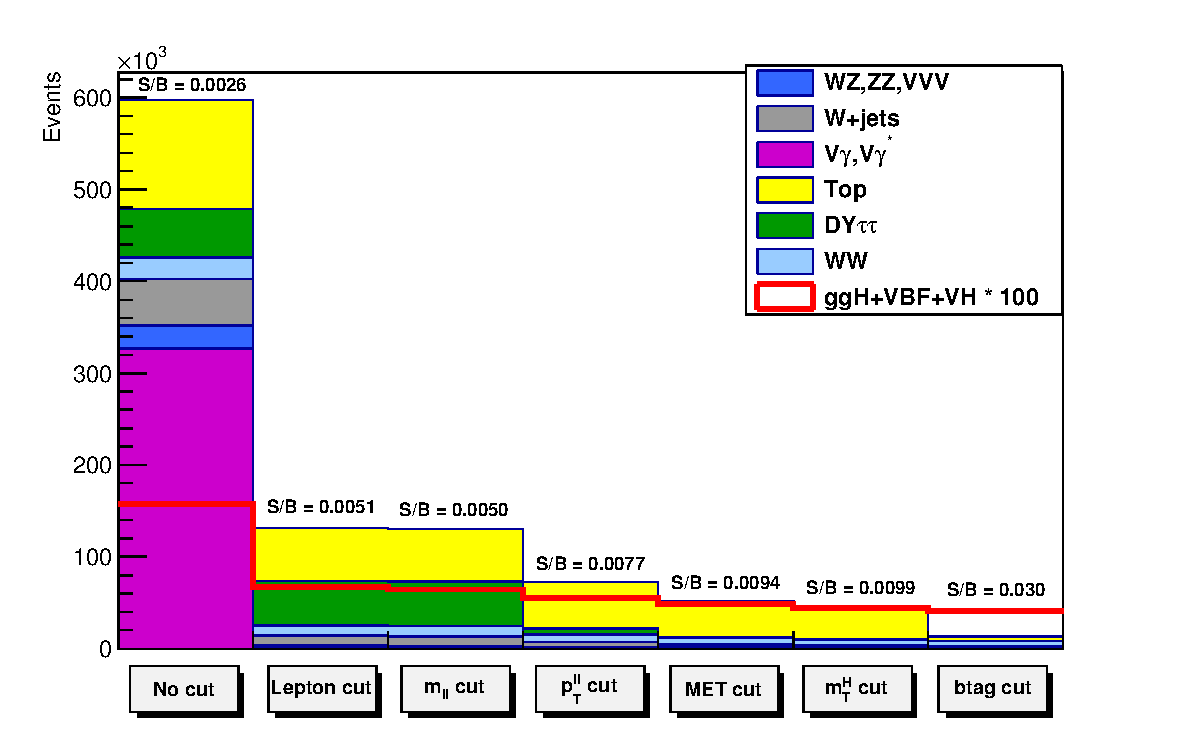
\includegraphics[width=0.8\textwidth]{images/cutflow2.pdf}
\caption{Effect of single selections on MC samples. The signal (red line) is multiplied by 100 and superimposed on stacked backgrounds. In each bin, corresponding to a different selection, is reported the expected number of events in MC at a luminosity of $19.46~\mathrm{fb}^{-1}$.\label{fig:cutflow}}
\end{figure}

A  cut-flow plot is reported in figure \ref{fig:cutflow} showing the effect of each selection on top of Monte Carlo samples. In the first bin, labelled as \textit{No cut}, no selection has been applied and the bin content correspond to the total expected number of events with a luminosity of $19.46~\mathrm{fb}^{-1}$. All the events in this bin have at least two leptons with a loose transverse momentum cut of $8$~\GeV. In the following bin the lepton cuts are applied, including the requirement to have two opposite-sign and opposite-flavour leptons and the extra lepton veto. Then are progressively reported all the other selections, showing the effect of each cut on backgrounds and signal. For each selection is also reported the expected signal over background ratio which after the full selection reach a maximum value around $3\%$.

\begin{figure}[t]
\centering
\subfigure[]{
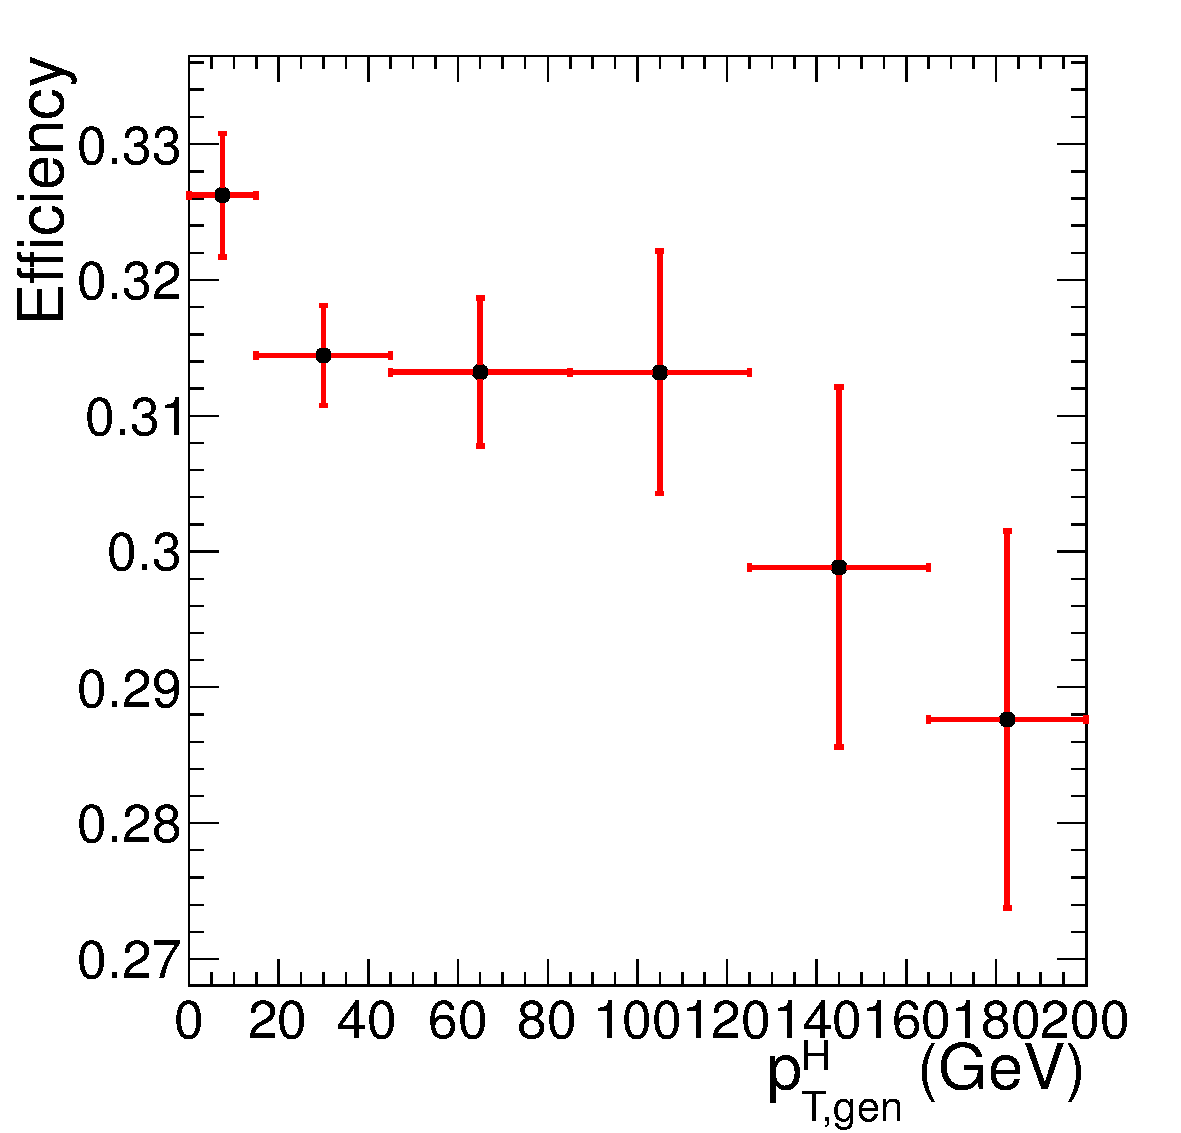
\includegraphics[width=0.4\textwidth]{images/eff_pth.pdf}
}
\subfigure[]{
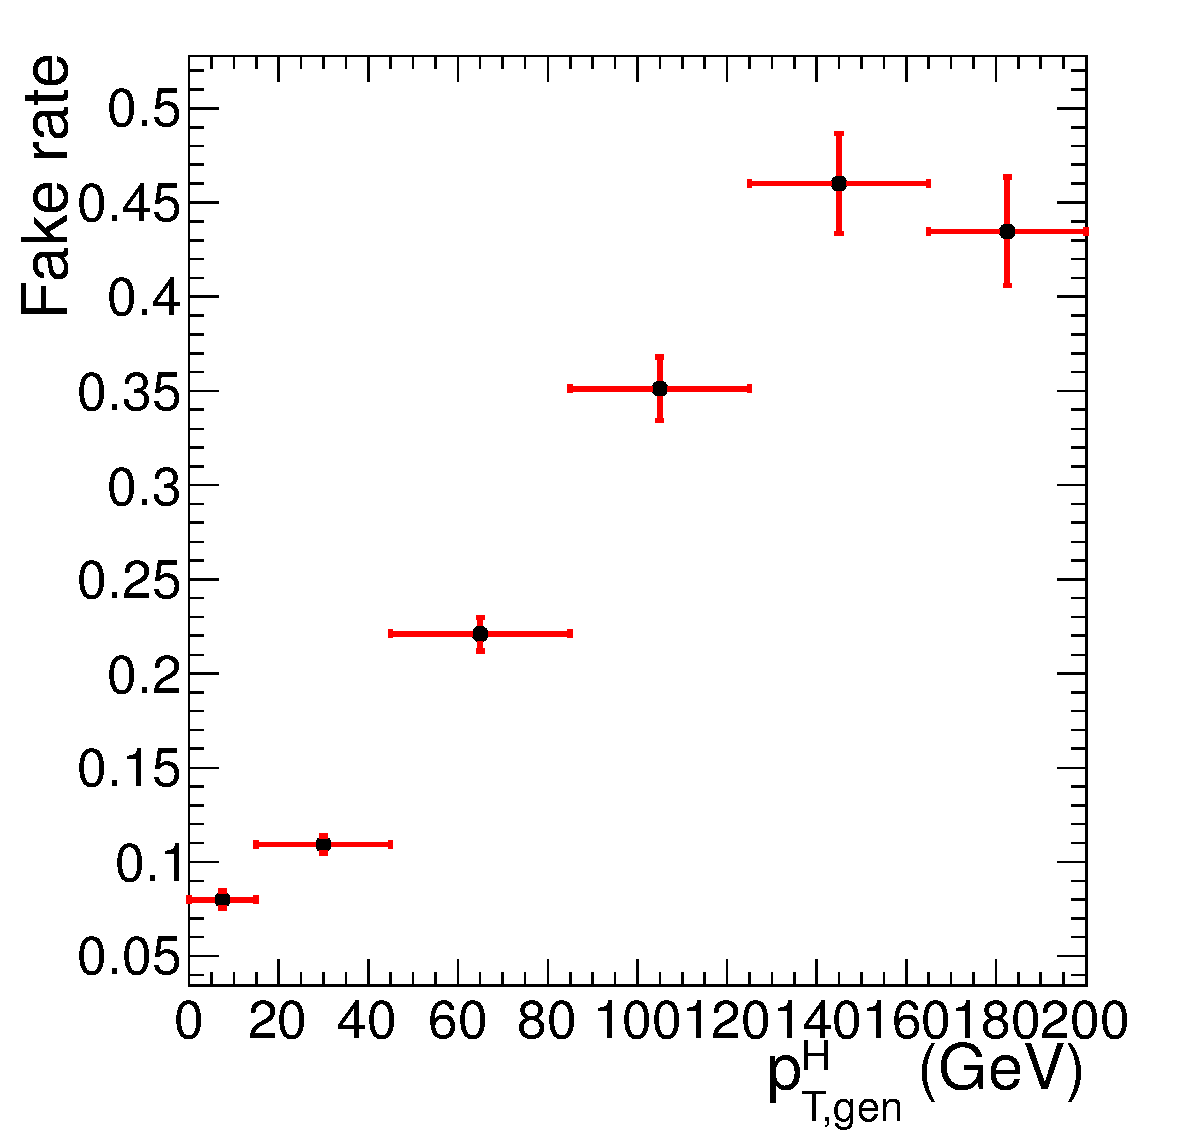
\includegraphics[width=0.4\textwidth]{images/fake_pth.pdf}
}
\caption{Efficiency of the full selection (a) and fake rate (b) as a function of $p_T^H$.\label{fig:sel_eff}}
\end{figure}

The selection efficiency is shown in Fig.~\ref{fig:sel_eff} (a). The efficiency denominator is the number of events that pass the acceptance, while the numerator is the number of events that pass both the selection and the acceptance, in each \pth bin. The fake rate, defined by the ratio of signal events that pass the selection but are not within the acceptance, divided by the total number of events passing both the selection and the acceptance is shown in Fig.~\ref{fig:sel_eff} (b). For both the selection efficiency and the fake rate the signal samples included correspond to the \textit{ggH}, \textit{VBF} and \textit{VH} production mechanisms.
The overall efficiency and fake rate are: $\epsilon=0.362\pm{0.005}$ and $fake~rate=0.126\pm0.004$, where the errors are only statistical.

If we define a $4\pi$ acceptance, requiring just that the Higgs decays to WW and then to $2l2\nu$, the efficiency is $\epsilon=0.03960\pm{0.00033}$. 


%\clearpage
%\section{Binning of the \pth spectrum}
%%%%%%%%%%%%%%%%%%%%%%%%%%%%%%%%%%%%%%%%%%%%%%%%%%%%%%%%%%%%%%%%%%%%%%
\label{sec:Binning}

Given the limited resolution on $\pth$, a criterion is needed to establish bi size. The criterion that we have chose is devised to keep under control the bin migrations due to the finite resolution. 
For any given bin $i$ we can define the purity $P_i$ on a signal sample as the number events that are generated and also reconstructed in that bin, $N_i^{GEN|RECO}$, divided by the number of events reconstructed there $N_i^{RECO}$:
\begin{equation}
P_i = \frac{N_i^{GEN|RECO}}{N_i^{RECO}} \qquad .
\end{equation}
Where $N_i^{GEN|RECO}$ is the number of events that are both generated and
reconstructed in a $\pth$ bin $i$, while $N_i^{RECO}$ is the number of events
that are reconstructed in bin $i$. We have chosen the bin width in such a way
as to make the smallest bins able to ensure a purity of about 60\% on a gluon fusion sample.
Following this prescription we have divided the whole $\pth$ range in six
different bins: \mbox{[0-15 GeV]}, \mbox{[15-45 GeV]}, \mbox{[45-85 GeV]},
\mbox{[85-125 GeV]}, \mbox{[125-165 GeV]}, \mbox{[165-$\infty$ GeV]}.
%Mettere plot binning
A two-dimensional histogram  has been made putting the GEN level $\pth$ on the x-axis (calculated using the WW system transverse momentum) and the RECO one on the y-axis. Each row is then normalized to one in order to directly have the purity in the diagonal bins. Also the effect of bin migration due to finite detector resolution effects can be assessed from this plot.\\
This two dimensional plot is shown in Fig.~\ref{fig:response_by_row} (a) and (b) for gluon fusion and VBF signals for $m_\mathrm{H}=125$\GeV.
\begin{figure}[b]
\centering
\subfigure[ggH]{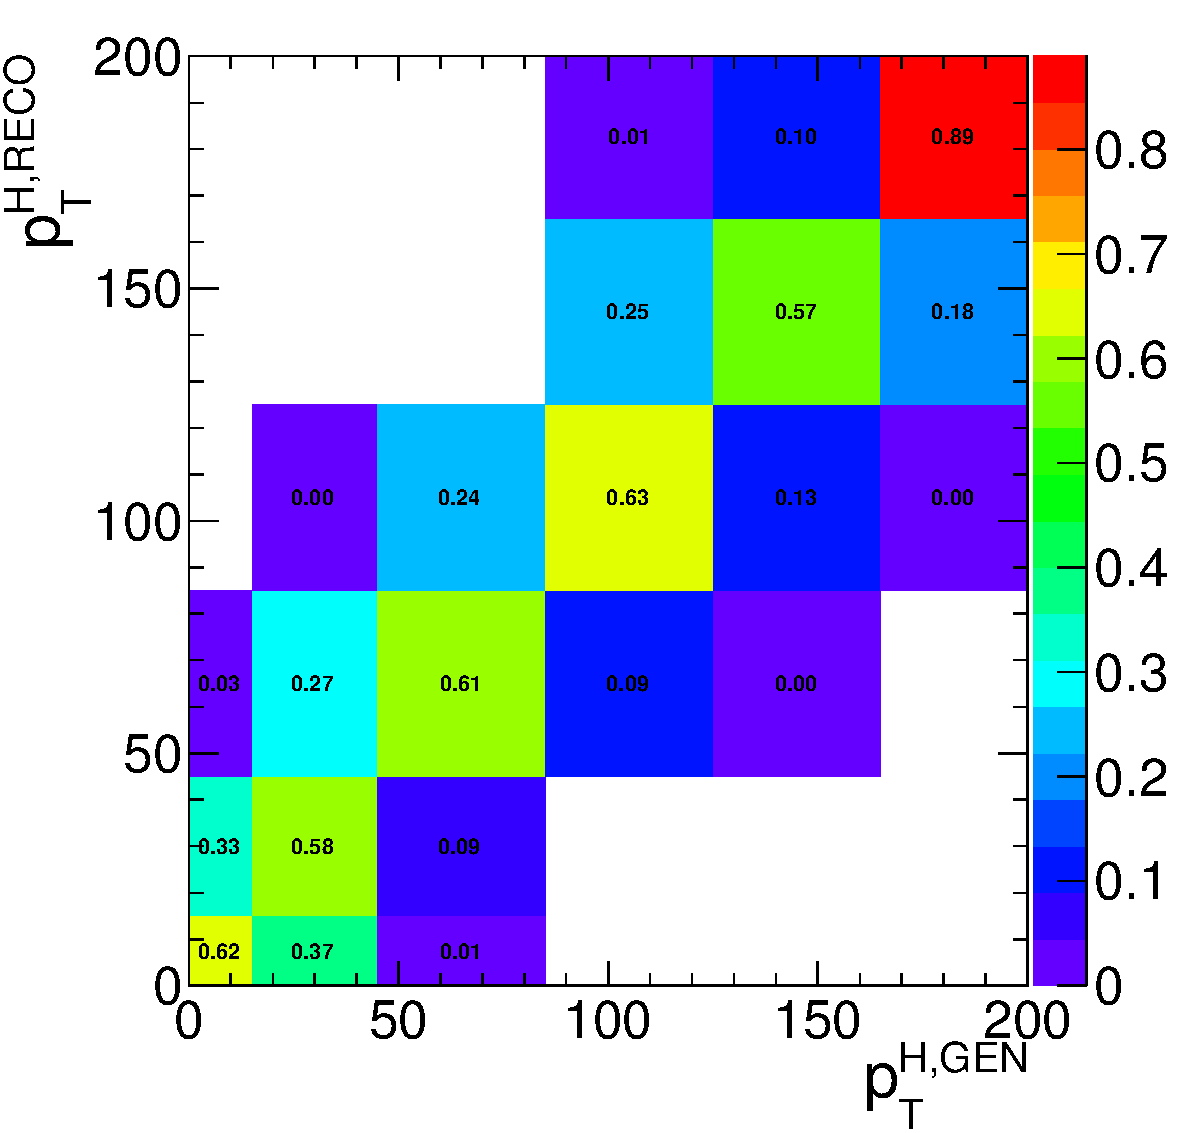
\includegraphics[width=0.45\textwidth]{images/response_ggH_norm_by_row.pdf}}
\subfigure[qqH]{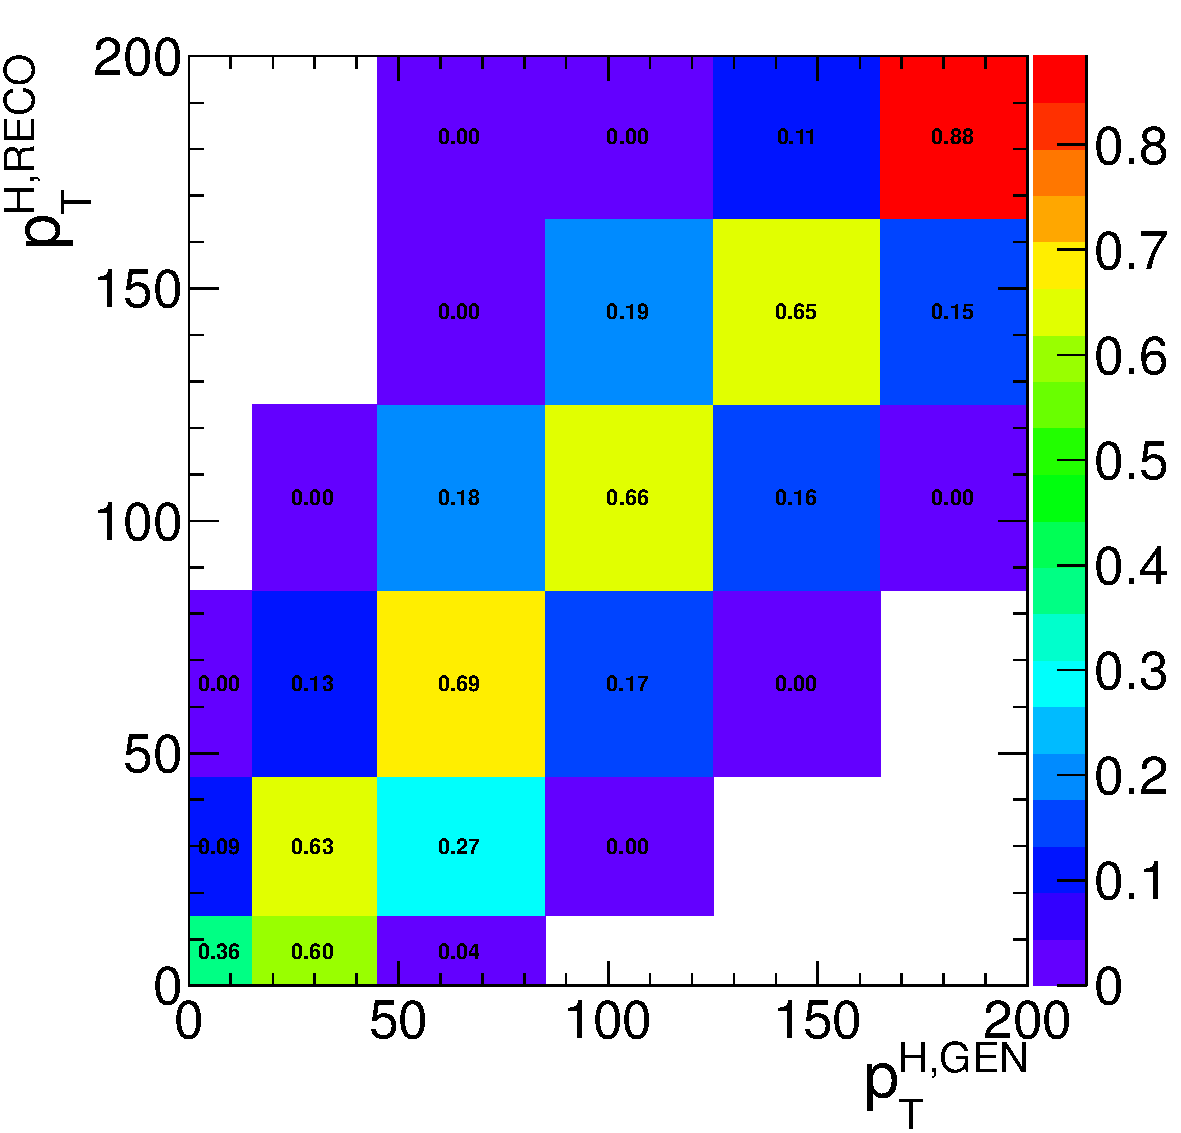
\includegraphics[width=0.45\textwidth]{images/response_qqH_norm_by_row.pdf}}
\caption{Reconstructed versus generated $\pth$ for gluon fusion (a) and VBF (b). Plots are normalized by rows, so that the bin purity is shown on the diagonal.\label{fig:response_by_row}}
\end{figure}

%\clearpage
\section{Background estimation}
%%%%%%%%%%%%%%%%%%%%%%%%%%%%%%%%%%%%%%%%%%%%%%%%%%%%%%%%%%%%%%%%%%%%%%
\label{sec:Backgrounds}

\textcolor{red}{Add plots for each background process}

\subsection{Top quark background \label{sec:TTBackground}}

In this analysis the top quark background is divided into two different categories depending on the number of jets in the event. In the two categories different selections are applied, especially concerning the b-tagging requirements.

The general strategy for determining the residual top events in the signal region is to first measure the top tagging efficiencies from an orthogonal region of phase space in data. The orthogonal phase space is  defined inverting the b-veto requirement of the signal region, in such a way to have a control region enriched in top quark events.  Then, using this efficiency, the number of events with the associated uncertainty is propagated from the control region to the signal region.
The number of surviving top events in the signal region would then be:

\begin{equation}
 N^{\mathrm{signal}}_{bveto} = N^{\mathrm{control}}_{btag} \cdot \frac{1-\epsilon_{\mathrm{top}}}{\epsilon_{\mathrm{top}}}
\label{eq:top_equation}
\end{equation}

where $N^{\rm control}_{\rm btag}$ is the number of events in the 
control region and $\epsilon_{\rm top}$ is the efficiency as measured
in data.

The methods to estimate the top background contribution in the two jet categories are different and are explained below.


\subsubsection{0-jets category}
Most of the top background, composed of \ttbar and tW processes, is rejected in the 0-jet bin by the
jet veto. The top-tagging efficiency in the zero jet bin, $\epsilon_{\rm tag}^{0-jet}$, is the probability for a top event to
fail one of either the b-tagging veto or the soft muon veto, and is defined as:

\begin{equation}\label{eq:eff_top_0j}
\epsilon_{\rm tag} = \frac{N_{\rm tag}^{\rm control}}{N^{\rm control}} \quad ,
\end{equation}

where $N^{\rm control}$ is the number of events in the top control phase space defined requiring one b-tagged jet with $\pt>30$\GeV, and $N_{\rm tag}^{\rm control}$ is the subset of those events that pass either the soft muon tagging or the low-\pt b jet tagging. The purity of this control sample, as estimated from simulation, is about 97\%. The remaining 3\% background contribution is estimated from simulation and subtracted from the numerator and denominator of Eq.~\eqref{eq:eff_top_0j}. The efficiency $\epsilon_{\rm top}^{0-jet}$ can then be estimated using the following formula:

\begin{equation}\label{eq:eff_top_0j}
\epsilon_{\rm top}^{0-jet} = f_{\ttbar} \cdot \epsilon_{2b} + f_{tW} \cdot ( x \cdot \epsilon_{2b} + (1-x) \cdot \epsilon_{\rm tag} ) \quad ,
\end{equation}

\begin{equation}
\epsilon_{2b} = 1 - (1 - \epsilon_{\rm tag})^{2} \quad ,
\end{equation}
where $f_{\ttbar}$ and $f_{tW}$ are the \ttbar and tW fractions respectively, $x$ is the fraction of tW events containing 2 b jets, and $\epsilon_{2b}$ is the efficiency for a top event with 0 counted jets, i.e. two soft b jets, to pass the top veto. For the ratio of \ttbar and tW cross-sections an uncertainty of 17\% is assumed. The fraction $f_{\ttbar}$ is estimated using MC simulation of the \ttbar and tW processes at NLO accuracy.

Using this procedure a data/simulation scale factor of $0.98 \pm 0.17$ is found, and is applied to correct the MC simulation in order to match the data.



\subsubsection{Category with more than 0 jets}
The strategy for the estimation of the top background in events with at least one jet with $\pt$ greater than 30 \GeV is the following. First of all the efficiency for tagging a b jet is measured both in data and simulation and the values are used to correct the simulation for different b-tagging efficiencies in data and simulation. This evaluation is performed in a control region, called CtrlTP, containing at least two jets, using a Tag\&Probe technique. The procedure to extract these scale factors is presented in Sec.~\ref{sec:TagAndProbe}. Then a larger statistics control region, CtrlDD, is defined by requiring at least one b-tagged jet and we use the simulation, corrected for the previously computed b-tagging efficiency scale factor, to derive the factor that connects the number of events in CtrlDD to the number of events in the signal region. This second step is explained in detail in Sec.~\ref{sec:DD}. 

\subsubsection{Tag\&Probe \label{sec:TagAndProbe}}
The Tag\&Probe technique is a method to estimate the efficiency of a selection on data. In can be applied whenever one has two objects in one event, by using one of the two, the \tg{}, to identify the process of interest, and using the second, the \probe{}, to actually measure the efficiency of the selection being studied. In our case we want to measure the b-tagging efficiency, so what we need is a sample with two b-jets per event. The easiest way to construct such a sample is to select $t\bar{t}$ events.

The CrtlTP control region is defined selecting the events which pass the lepton preselection cuts listed in Sec.~\ref{subsec:EventSelection}, and have at least two jets with \pt greater than 30 \GeV.
One of the two leading jets is required to have a \jpb score higher than 0.5. From events in this control region we built \tp{} pairs as follows. For each event the two leading jets are considered. If the leading jet passes the \jpb cut of 0.5, that is considered a \tg{}, and the sub-leading jet is the \probe{}. In order to avoid any bias that could arise from the probe being always the second jet, the pair is tested also in reverse order, meaning that the sub-leading jet is tested against the \tg{} selection, and in case it passes, then the leading jet is used as \probe{} in an independent \tp{} pair. This means that from each event passing the CrtlTP cuts one can build up to two \tp{} pairs. 

If the \tg{} selection were sufficient to suppress any non top events, one could estimate the efficiency by dividing the number of \tp{} pairs in which the \probe{} passes the analysis cut \jpb$>$1.4 (\tpp) by the total number of \tp{} pairs. However this is not the case. 
In order to estimate the efficiency in the presence of background a variable that discriminates between true b-jets and other jets in a $t\bar{t}$ sample is chosen. The variable is the \pt of the \probe{} jet. For real b-jets this variable has a peak around 60 \GeV, while it does not peak for other jets. The idea is to fit simultaneously the \pt spectrum for \probe{} jets in \tpp{} and \tfp{} pairs, linking together the normalizations of the two samples as follows:
\begin{equation}
N_{TPP}=N_{s}\epsilon_{s} + N_b\epsilon_{b}
\end{equation}
\begin{equation}
N_{TFP}=N_{s}(1-\epsilon_{s}) + N_b(1-\epsilon_{b})
\end{equation}
where $N_{\rm TPP}$ is the number of \tpp{} pairs, $N_{\rm TFP}$ is the number of \tfp{} pairs, $N_{\rm s}$ is the number of \tp{} pairs in which the probe is a b-jet, $N_{\rm b}$ is the number of \tp{} pairs in which the probe is a not b-jet, $\epsilon_{\rm s}$ is the b-tagging efficiency, $\epsilon_{\rm b}$ is the probability of identifying as b-jet a non-b-jets, i.e. the mistag rate. 

A $\chi^{2}$ simultaneous fit of the \probe{} \pt spectrum for \tpp{} and \tfp{} pairs is performed, deriving the shapes for true b-jets and non-b-jets from the simulation, and extracting $N_{\rm s}$, $N_{\rm b}$, $\epsilon_{\rm s}$ and $\epsilon_{\rm b}$ from the fit.
The result of the fit on simulation is shown in Fig.~\ref{fig:mc_tp}. The relevant efficiencies are:
\begin{equation}
\epsilon_{s}^{MC}=0.7663\pm0.0072
\end{equation}
\begin{equation}
\epsilon_{b}^{MC}=0.208\pm0.015
\end{equation}
We have checked that these values are consistent with the true value for the b-tagging efficiency. The true value is computed by selecting jets that are matched within a cone of $\Delta{R}<0.5$ with a generator level b-quark, and counting the faction of those that pass the \jpb cut of 1.4. This means that the \tp{} method does not introduce biases within the simulation statistic accuracy.

\begin{figure}[b]
\centering
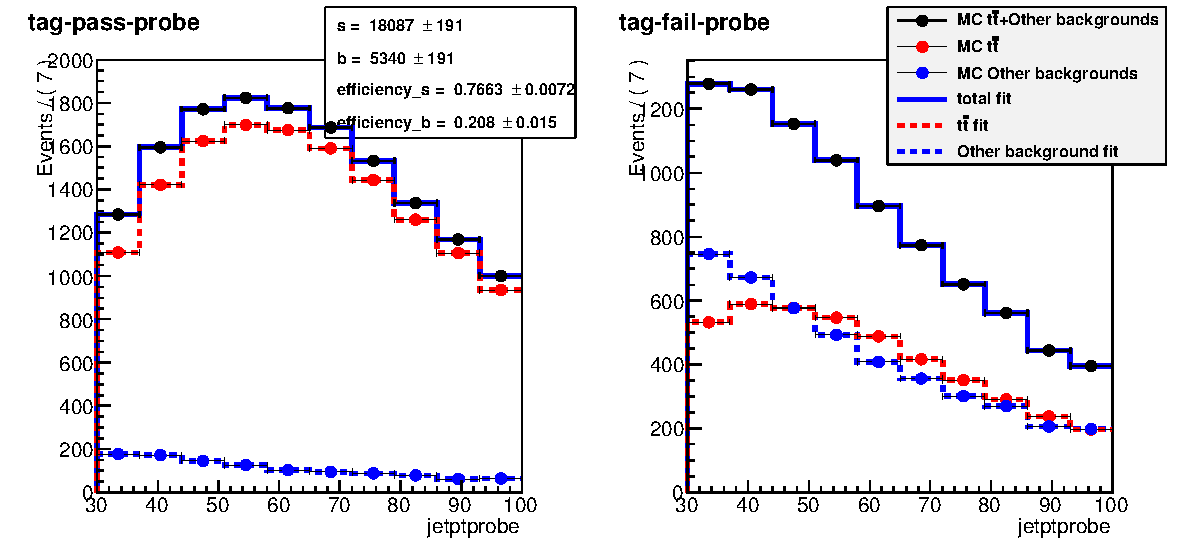
\includegraphics[width=0.8\textwidth]{images/mc_pt_probe.pdf}
\caption{Simultaneous fit of the \tpp{} and \tfp{} pairs in the MC.\label{fig:mc_tp}}
\end{figure}

In order to assess the robustness of the fit, 5000 toy MC samples have been generated with a statistics equivalent to the one expected in data and the same fit is performed. All the 5000 fit succeeded, and the pull distributions for $\epsilon_{\rm s}$ and $\epsilon_{\rm b}$ parameters are shown in Fig.~\ref{fig:pullstp}. The plots show the pull of the efficiencies measured in the fit, where the pull variable for each toy $i$ is defined as:

\begin{equation}
pull(\epsilon_{\rm s (b)}) = \frac{\epsilon_{\rm s (b)}^{\rm true} - \epsilon_{\rm s (b)}^{i}}{\sigma(\epsilon_{\rm s (b)}^{i})}
\end{equation}

The pulls are centered on 0 and have $\sigma$ close to 1, as expected.

\begin{figure}[t]
\centering
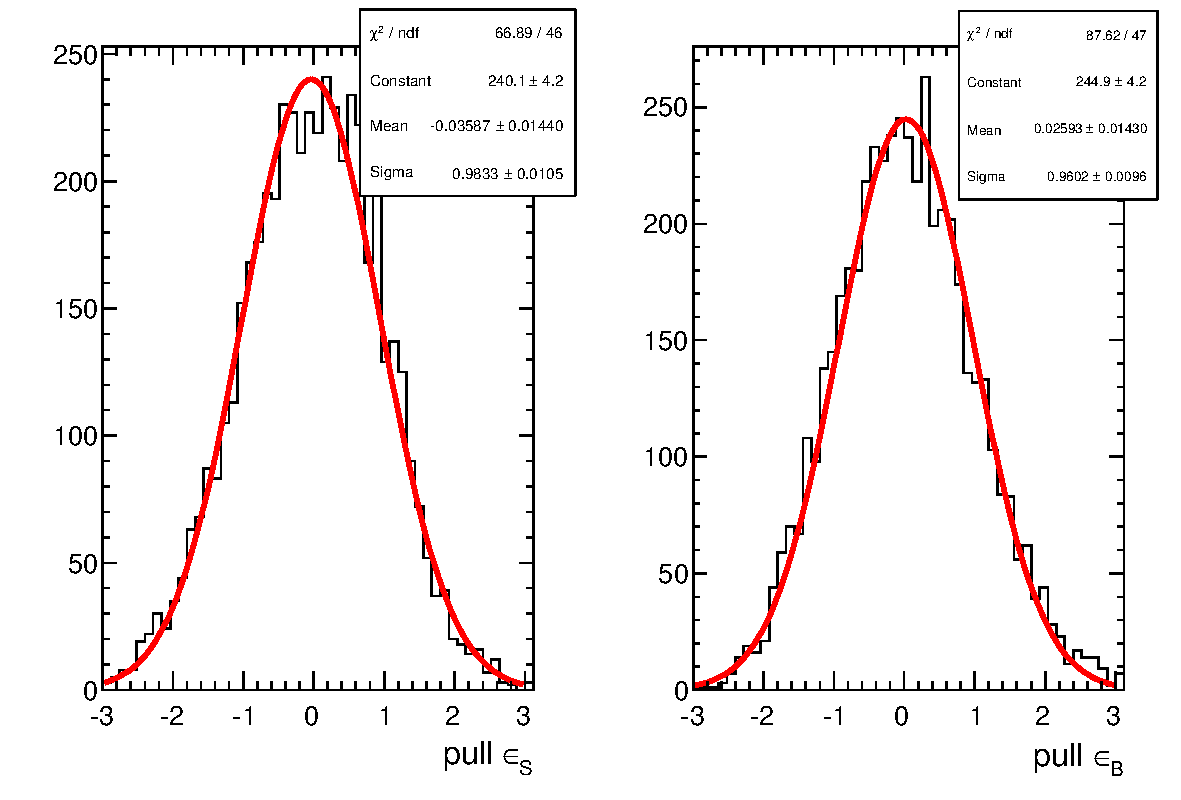
\includegraphics[width=0.8\textwidth]{images/pulls_mc.pdf}
\caption{Pulls of the $\epsilon_{s}$ and $\epsilon_{b}$ parameters in 5000 toy MC.\label{fig:pullstp}}
\end{figure}
An example fit for one of the toys is shown in  Fig.~\ref{fig:toy_tp}
\begin{figure}[b]
\centering
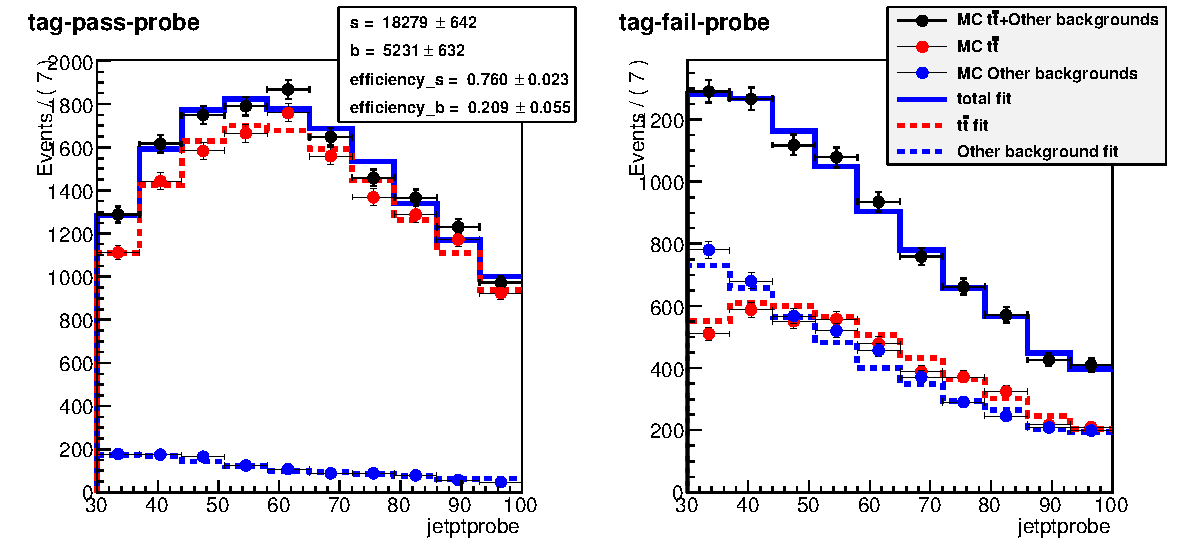
\includegraphics[width=0.8\textwidth]{images/mc_pt_probe_toy.pdf}
\caption{Fit of a toy MC sample.\label{fig:toy_tp}}
\end{figure}

Before running the fit on data, the shapes used in the fit have been validated. To do so, a purer top enriched phase space has been defined by requiring exactly two jets with \jpb score higher than 1.5 and no additional b-tagged jets, rejecting also jets with \pt smaller than 30 \GeV. On this purer sample we have compared data against the shape used to fit the true b-jets in the \tpp{} distribution. The result is shown in Fig.~\ref{fig:purett} and shows good agreement.
\begin{figure}[t]
\centering
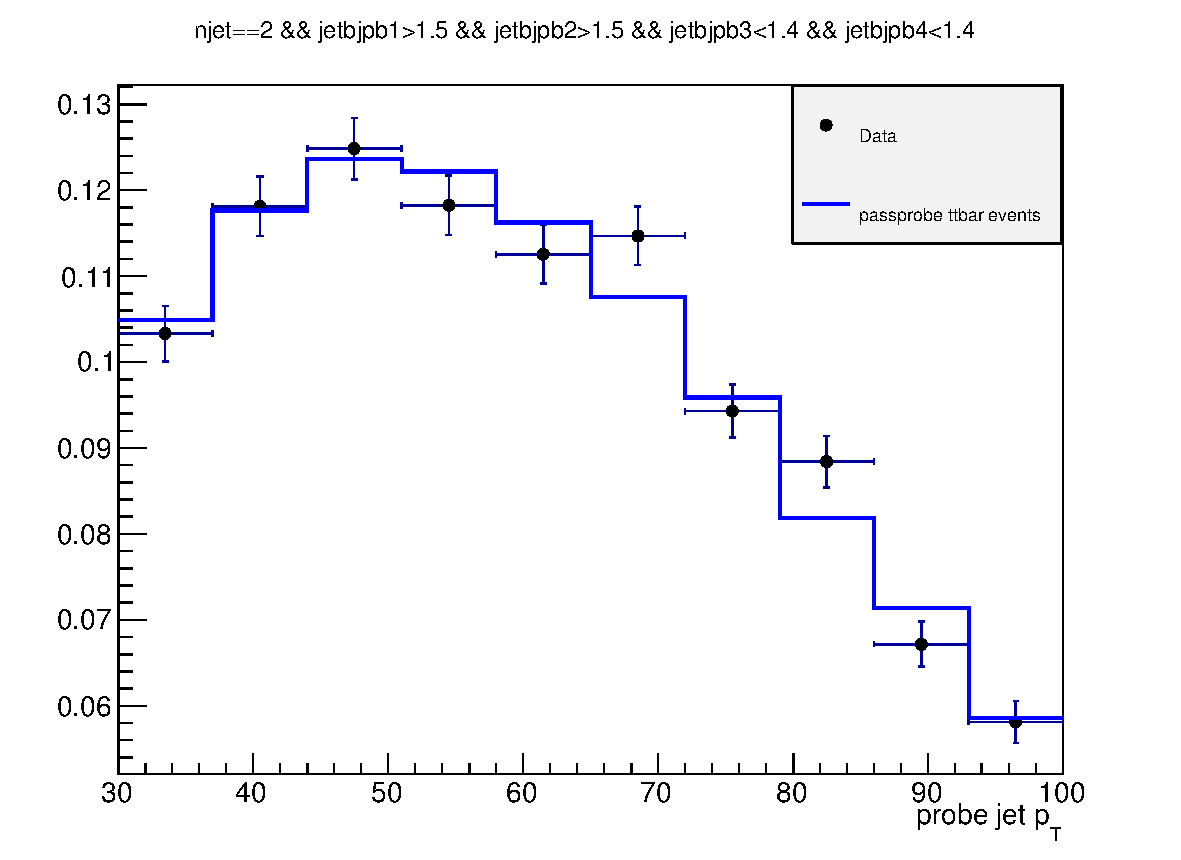
\includegraphics[width=0.6\textwidth]{images/passprobe_data_mc.pdf}
\caption{Shape comparison for the \probe{} \pt spectrum in data and in MC in a very pure \ttbar sample.\label{fig:purett}}
\end{figure}

Finally the fit has been performed on data, as shown in Fig.~\ref{fig:data_tp}, providing the following efficiencies:
\begin{equation}
\epsilon_{s}^{Data}=0.769\pm0.022
\end{equation}
\begin{equation}
\epsilon_{b}^{Data}=0.121\pm0.054
\end{equation}

\begin{figure}[b]
\centering
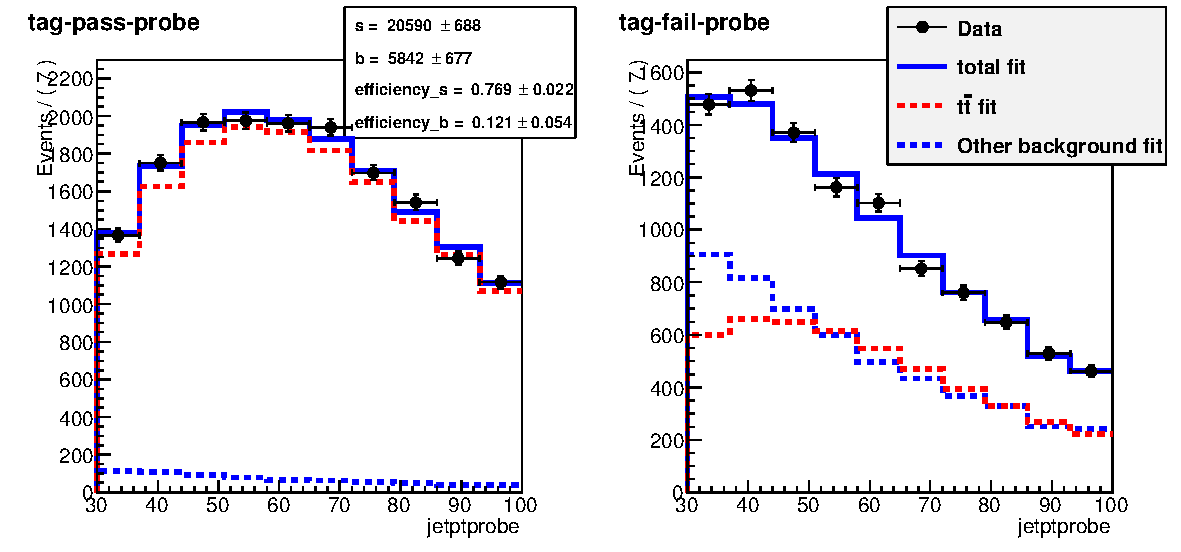
\includegraphics[width=0.8\textwidth]{images/data_ptprobe.pdf}
\caption{Simultaneous fit of the \tpp{} and \tfp{} pairs in data.\label{fig:data_tp}}
\end{figure}

Further studies have been performed to assess the effect of the relative uncertainty on the \ttbar and tW event fractions. The same procedure described above has been applied to different simulation templates obtained varying the \ttbar and tW fractions within theoretical uncertainties, and the effect on the parameters extracted with the fit procedure is found to be well below the fit uncertainties.


\subsubsection{Data driven estimation \label{sec:DD}}
In addition to the b-tagging efficiency, the other ingredient to estimate the \ttbar background is the process cross section. The idea is to measure the cross section in a \ttbar enriched control region, that is called CtrlDD. CtrlDD is defined according to the lepton preselection cuts defined in Sec.~\ref{sec:Selections}, and requiring in addition at least one jet with \jpb score higher than 1.4.

From the simulation we derive the factor $\alpha$ that connects CrtlDD to the signal region, calculating the ratio of \ttbar events in the two regions:

\begin{equation}
\alpha=\frac{N_{\ttbar~MC}^{SIG}}{N_{\ttbar~MC}^{CtrlDD}} \quad.
\end{equation}

The number of events in the CtrlDD region in data is counted, subtracting the expected number of events from non-\ttbar backgrounds, and obtaining $N_{\ttbar~Data}^{CtrlDD}$. Finally the number of expected \ttbar events in the signal region ($N_{\ttbar~Data}^{SIG}$) is obtained as:

\begin{equation}
N_{\ttbar~Data}^{SIG} = \alpha{}N_{\ttbar~Data}^{CtrlDD}.
\end{equation}

In evaluating $\alpha$ and its error the b-tagging efficiencies determined in Sec.~\ref{sec:TagAndProbe} are used. 
For each event an efficiency scale factor and a mistag rate scale factor are derived, depending on whether the event falls in the signal or CtrlDD region.

\begin{equation}
\label{eq:sfsig}
SF_{SIG} = \left(\frac{1-\epsilon_{s}^{Data}}{1-\epsilon_{s}^{MC}}\right)^{min(2, n_{b-jets})} \left(\frac{1-\epsilon_{b}^{Data}}{1-\epsilon_{b}^{MC}}\right)^{n_{non-b-jets}} 
\end{equation}

\begin{equation}
\label{eq:sfbkg}
SF_{CtrlDD} = \left(\frac{\epsilon_{s}^{Data}}{\epsilon_{s}^{MC}}\right)^{(jet1 == b-jet)} \left(\frac{\epsilon_{b}^{Data}}{\epsilon_{b}^{MC}}\right)^{(jet1 == non-b-jets)} 
\end{equation}

where $n_{b-jets}$ is the number of true b-jets in the event and $n_{non-b-jets}$ is the number of non-b-jets in the event. The writing $jet1 == b-jet$ ($jet1 == non-b-jets$) is a boolean flag that is true when the leading jet, the one used for the CtrlDD selection, is (not) a true b-jet.

Since the efficiency and mistag rate that have been measured on data are close to the one in the simulation, it was decided to assume a scale factor of 1 for both b-tagging efficiency and mis-tag rate. This means that the central values of the scale factors defined in Eq.~\ref{eq:sfsig} and Eq.~\ref{eq:sfbkg} is 1, but these numbers have an error that is derived assuming an uncertainty on $\epsilon_{s}^{Data}$ and $\epsilon_{b}^{Data}$ that covers both the statistical error from the fit of the two quantities and the difference with respect to the simulation.
This results in an up and a down variation of the scale factors in the signal and CtrlDD regions, that is used to derive an error on $\alpha$.

A data driven estimation of the top quark background with the method described above is performed in each of the \pth bins independently. The reason to make this estimation in $\pth$ bins, rather than inclusively is explained in Fig.~\ref{fig:ttpth}, where the \pth distribution is shown in the CtrlDD region normalized to the cross section measured by a specific CMS analysis~\cite{Khachatryan:2016mqs}. As shown in the ratio plot, an overall normalization factor would not be able to accommodate for the variations of the data/simulation ratio from bin to bin.

\begin{figure}[b]
\centering
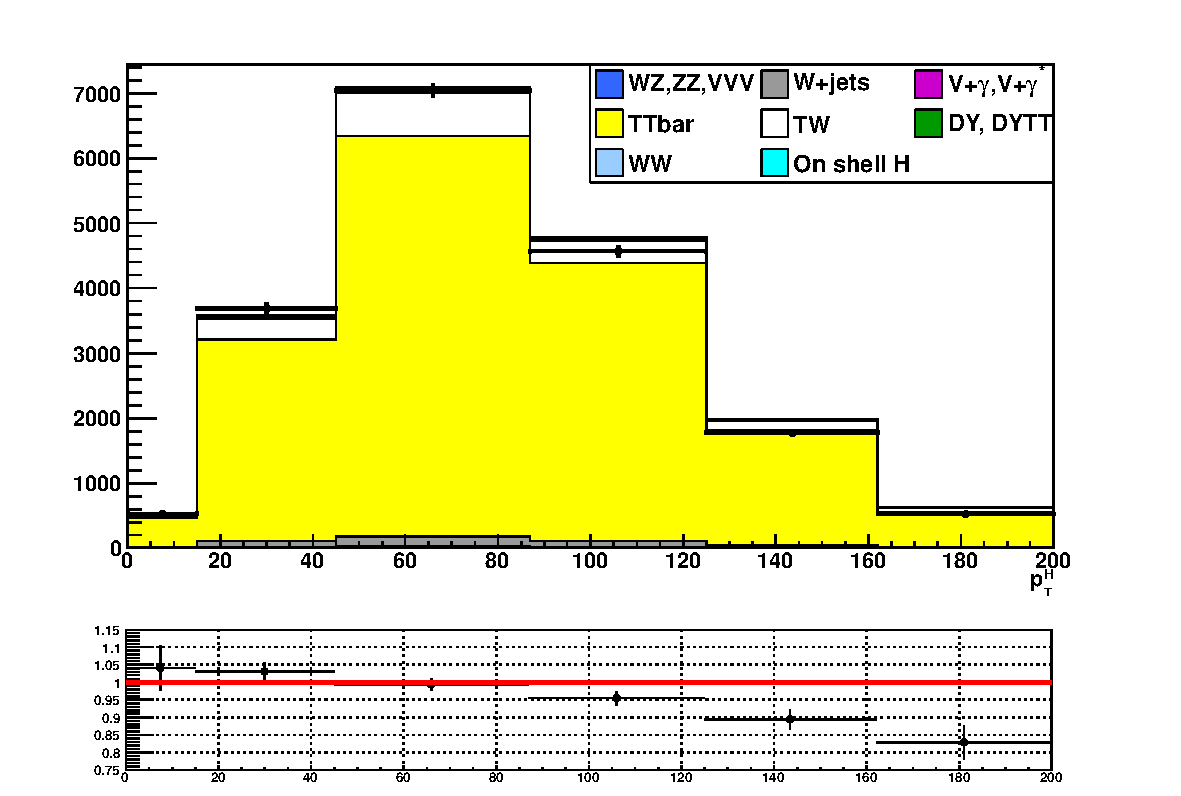
\includegraphics[width=0.6\textwidth]{images/ttpth.pdf}
\caption{$\pth$ distribution in the CtrlDD control region.\label{fig:ttpth}}
\end{figure}

The $\alpha$ factors for each bin and the number of events in signal, CtrlDD regions in MC as well as in data are listed in Tab.~\ref{tab:ttdd}.
\begin{table}
\centering
\begin{tabular}{c c c c c c}
\hline
\pth [\GeV] & $N_{CTRL}^{DATA}$ & $N_{CTRL}^{TOP}$ &  $N_{SIG}^{TOP}$ &
$\alpha$ & $\Delta\alpha$ \\ 
\hline\hline
$[0--15]$ & 406.71 & 358.78 & 117.83 & 0.328 & 0.075 \\ 
$[15--45]$ & 2930.14 & 2703.44 & 859.08 & 0.318 & 0.071 \\ 
$[45--85]$ & 5481.02 & 5207.48 & 1506.05 & 0.289 & 0.065 \\ 
$[85--125]$ & 4126.35 & 4032.56 & 861.22 & 0.214 & 0.052 \\ 
$[125--165]$ & 1612.64 & 1654.27 & 304.69 & 0.184 & 0.055 \\ 
$[165--\infty]$ & 647.50 & 760.37 & 201.70 & 0.265 & 0.147 \\ 
\hline
\end{tabular}
\caption{Data driven scale factors related to the top quark background estimation.\label{tab:ttdd}}
\end{table}

A comparison of the $\mll$ distribution in the six $\pth$ bins used in the analysis in CtrlDD after the data driven correction is shown in Fig.~\ref{fig:mllCtrlDD}
\begin{figure}[htb]
\centering
\subfigure[$\pth<15\GeV$]{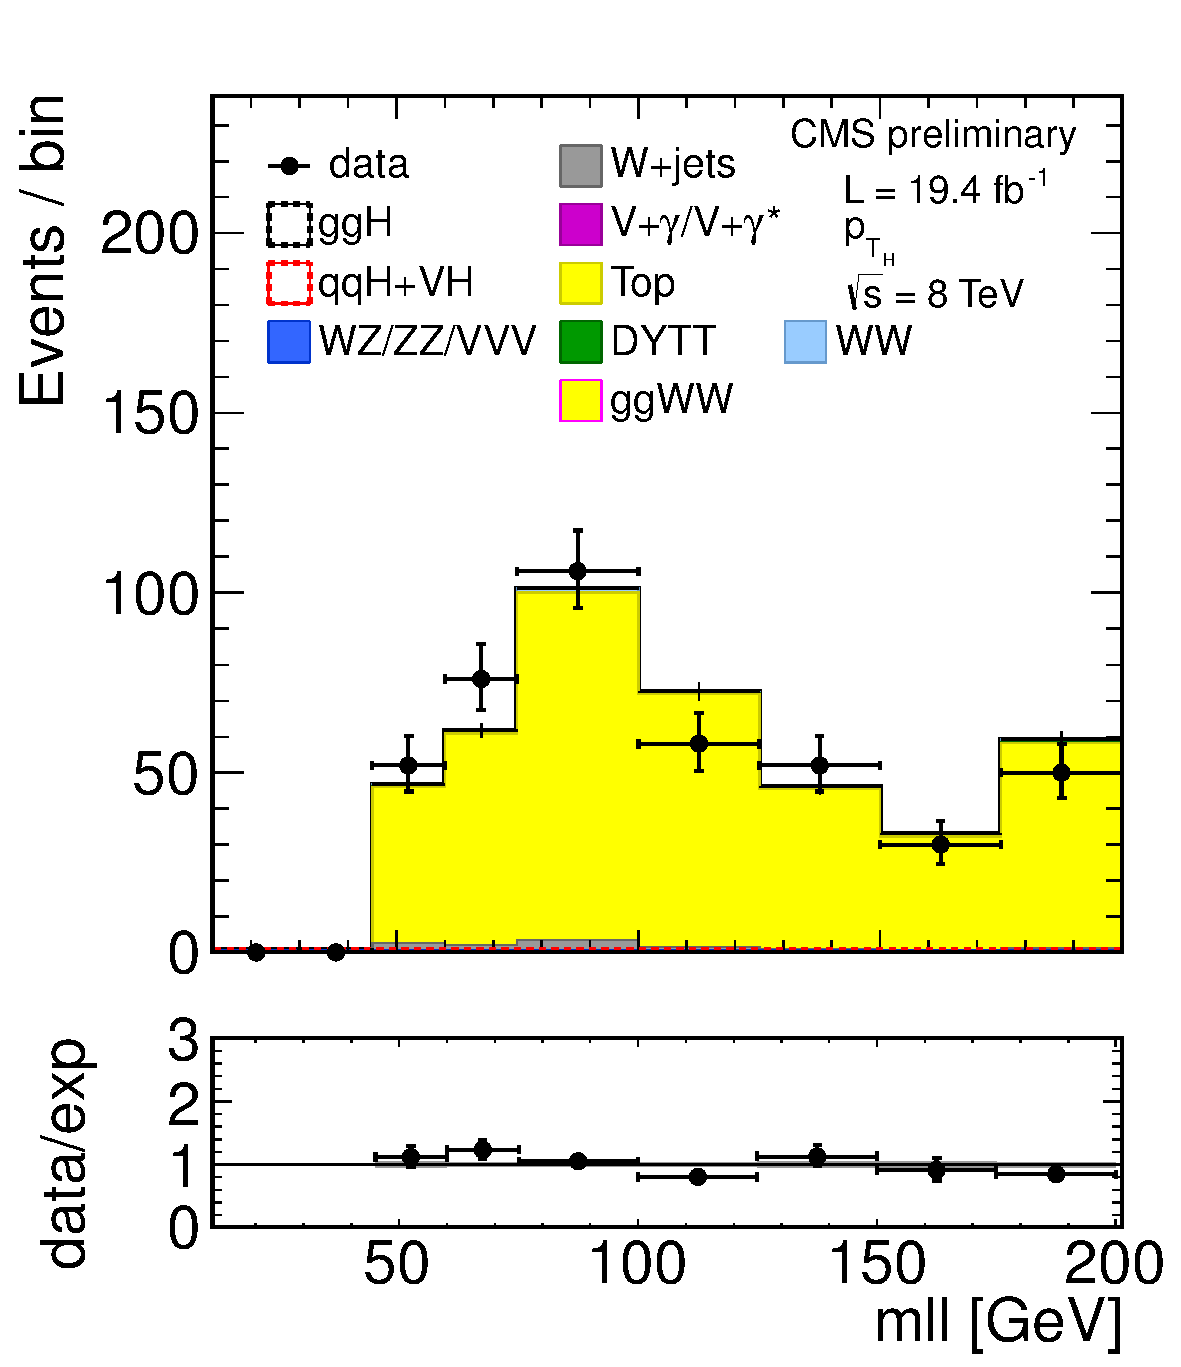
\includegraphics[width=0.35\textwidth]{images/mllBin0CtrlDD.pdf}}
\subfigure[$15\GeV<\pth<45\GeV$]{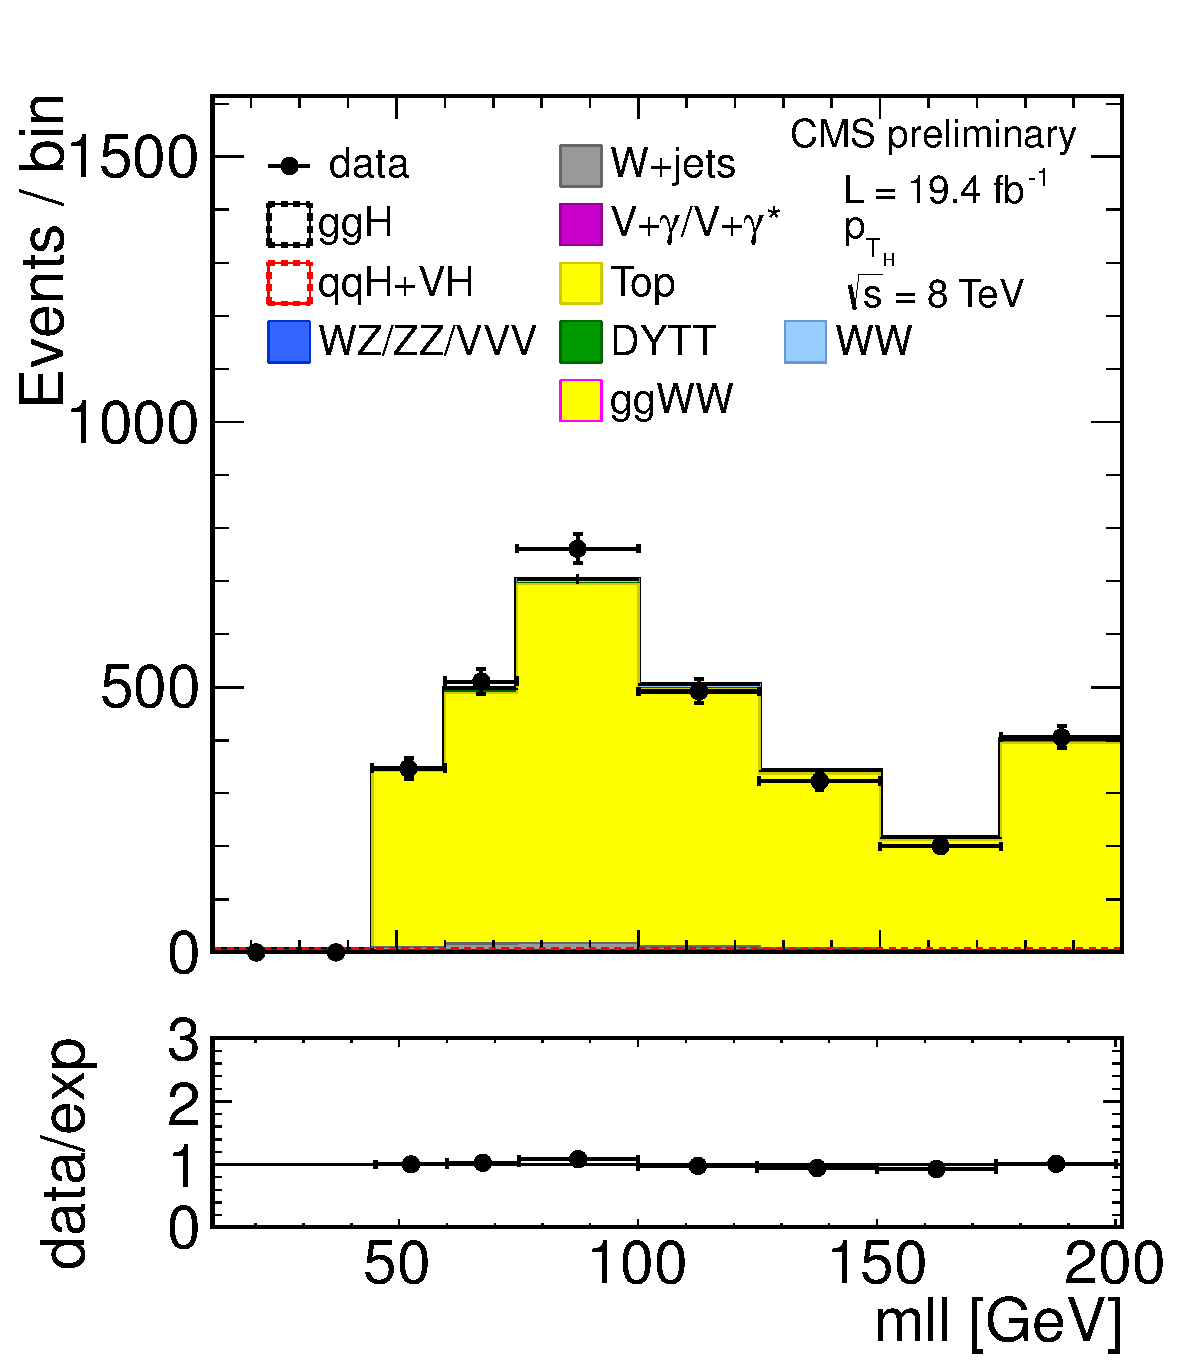
\includegraphics[width=0.35\textwidth]{images/mllBin1CtrlDD.pdf}}

\subfigure[$45\GeV<\pth<85\GeV$]{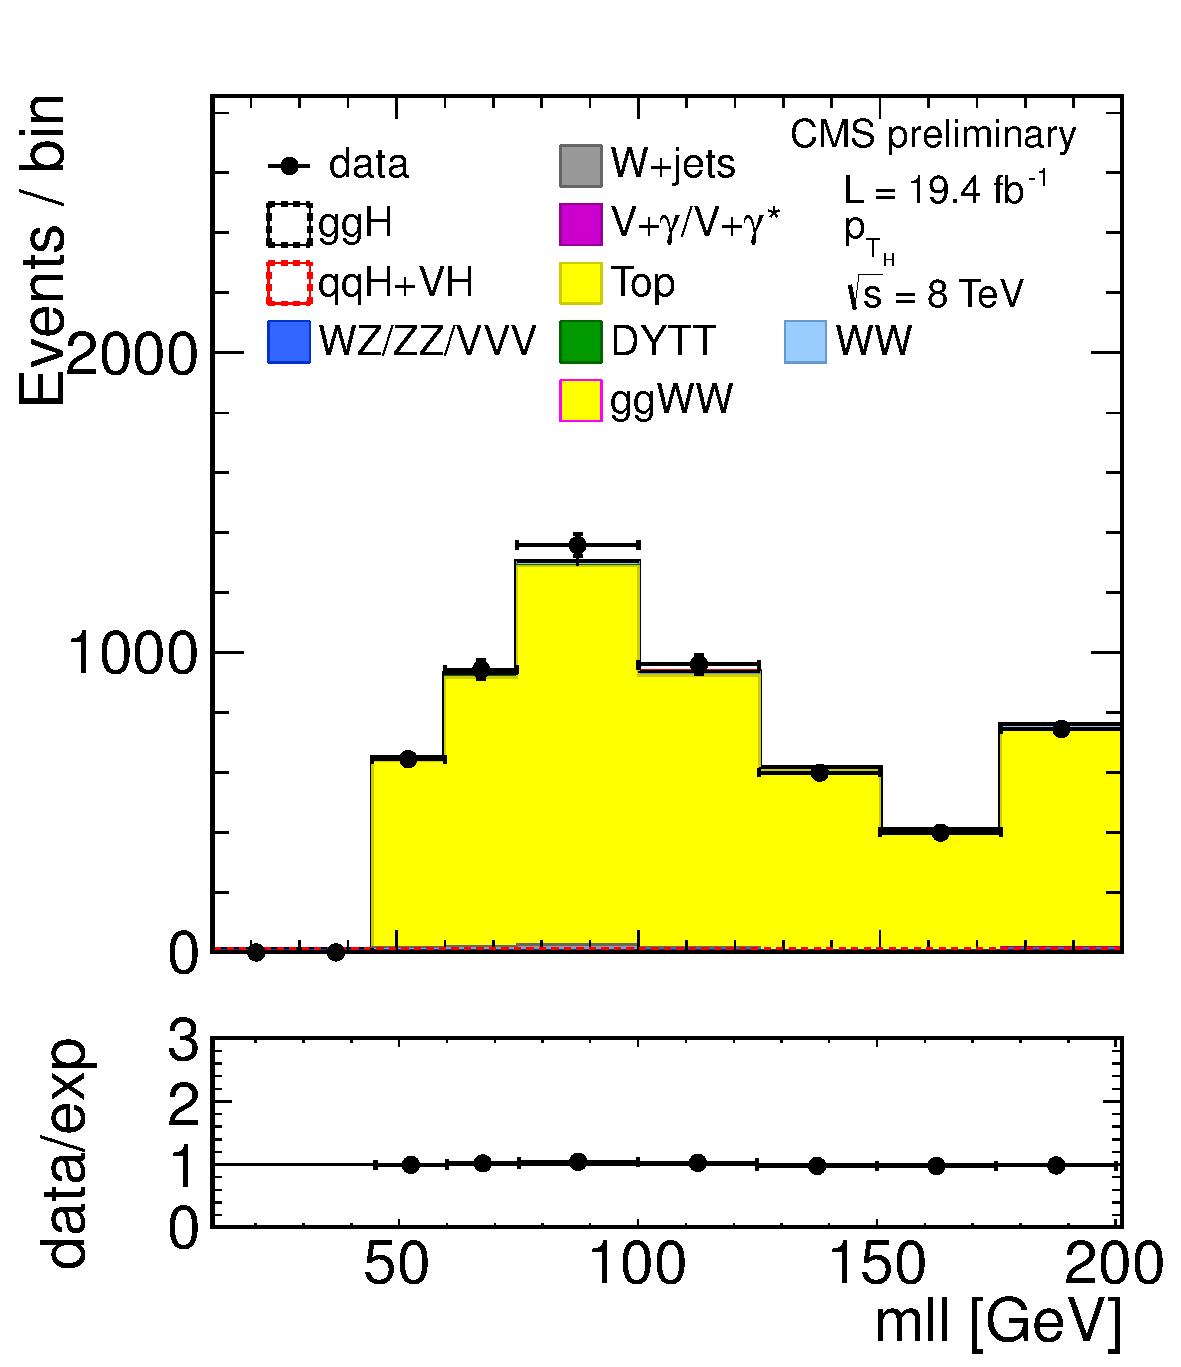
\includegraphics[width=0.35\textwidth]{images/mllBin2CtrlDD.pdf}}
\subfigure[$85\GeV<\pth<125\GeV$]{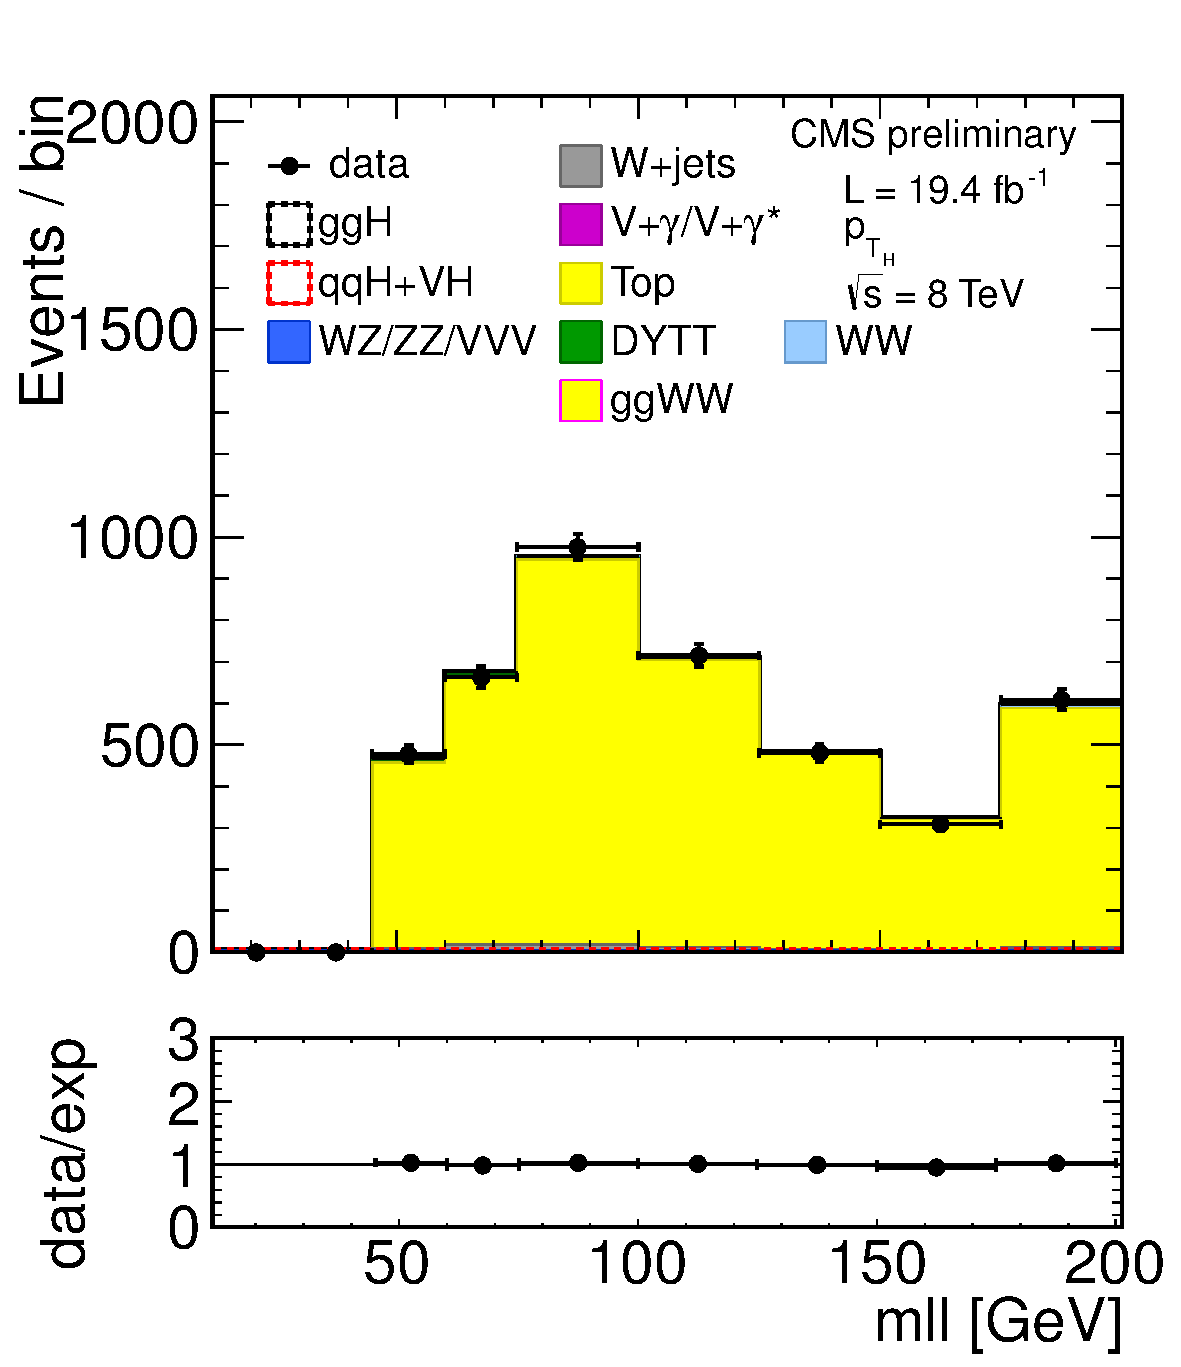
\includegraphics[width=0.35\textwidth]{images/mllBin3CtrlDD.pdf}}

\subfigure[$125\GeV<\pth<165\GeV$]{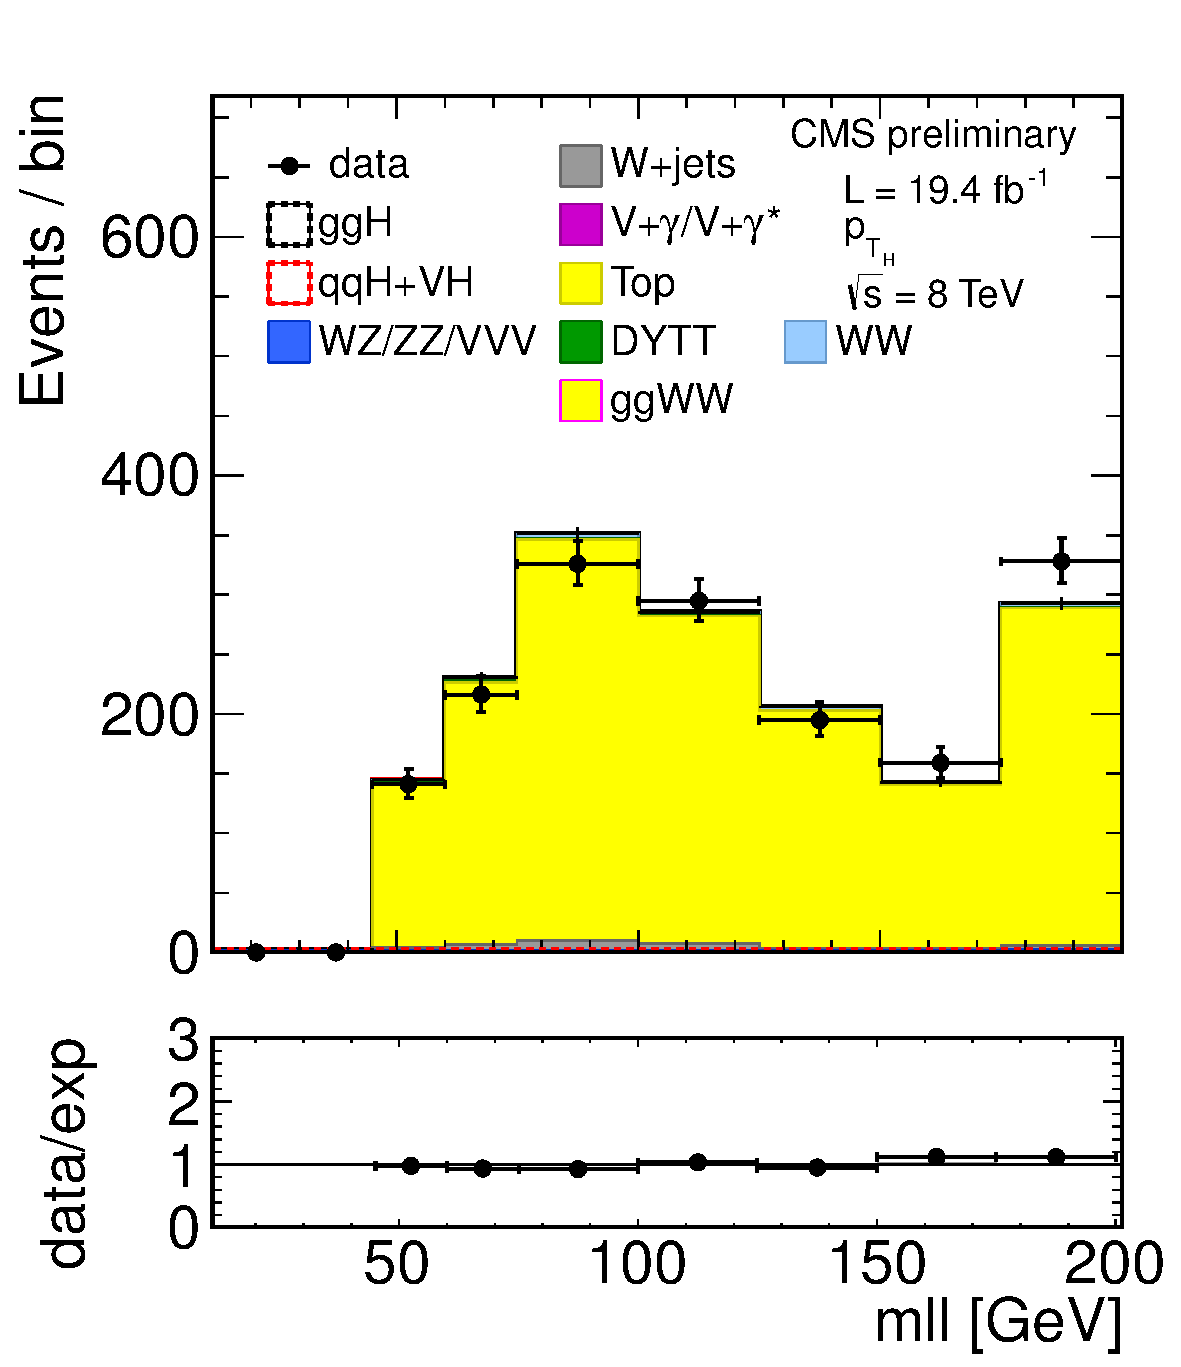
\includegraphics[width=0.35\textwidth]{images/mllBin4CtrlDD.pdf}}
\subfigure[$\pth>165\GeV$]{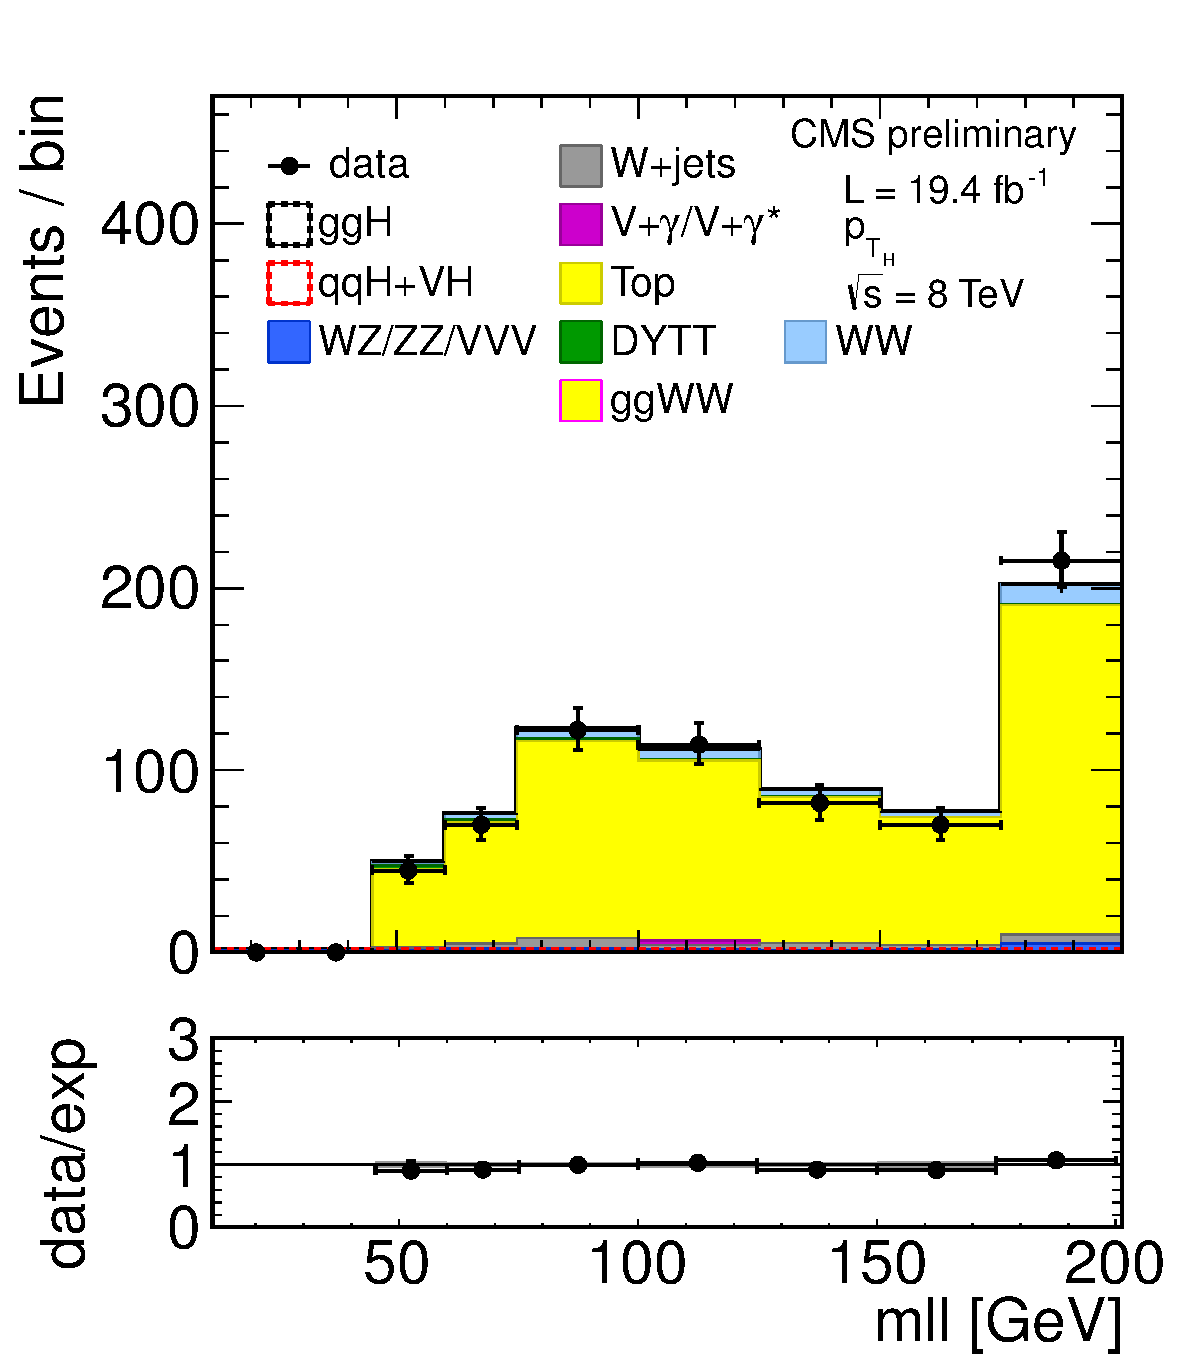
\includegraphics[width=0.35\textwidth]{images/mllBin5CtrlDD.pdf}}
\caption{$\mll$ distributions in the CtrlDD region for the different $\pth$ bins.\label{fig:mllCtrlDD}}
\end{figure}

























\clearpage
\subsection{WW background \label{sec:WWBackground}}

For what the $\mathrm{qq\to W^{+}W^{-}}$ background shape is concerned, the prediction from the simulation is used.
This background is divided into six different parts, corresponding to the six \pth bins defined in the analysis. The normalization of the $\mathrm{qq\to W^{+}W^{-}}$ background is left free to float in each bin, in such a way to adjust it in order to match the data during the fit procedure. In this way we minimize the shape difference between the $p_\mathrm{T}^\mathrm{WW}$ theory prediction and the distribution provided by the simulation, in our case the \textsc{Madgraph} generator.\\
In figure \ref{fig:ww_wwnlo} a comparison is shown between the $p_\mathrm{T}^\mathrm{WW}$ spectra of two different $\mathrm{qq\to W^{+}W^{-}}$ samples: one obtained with the \textsc{Madgraph} generator and the other after applying to the same distribution a reweighting in order to match the theoretical prediction at NLO+NNLL precision.

\begin{figure}[b]
\centering
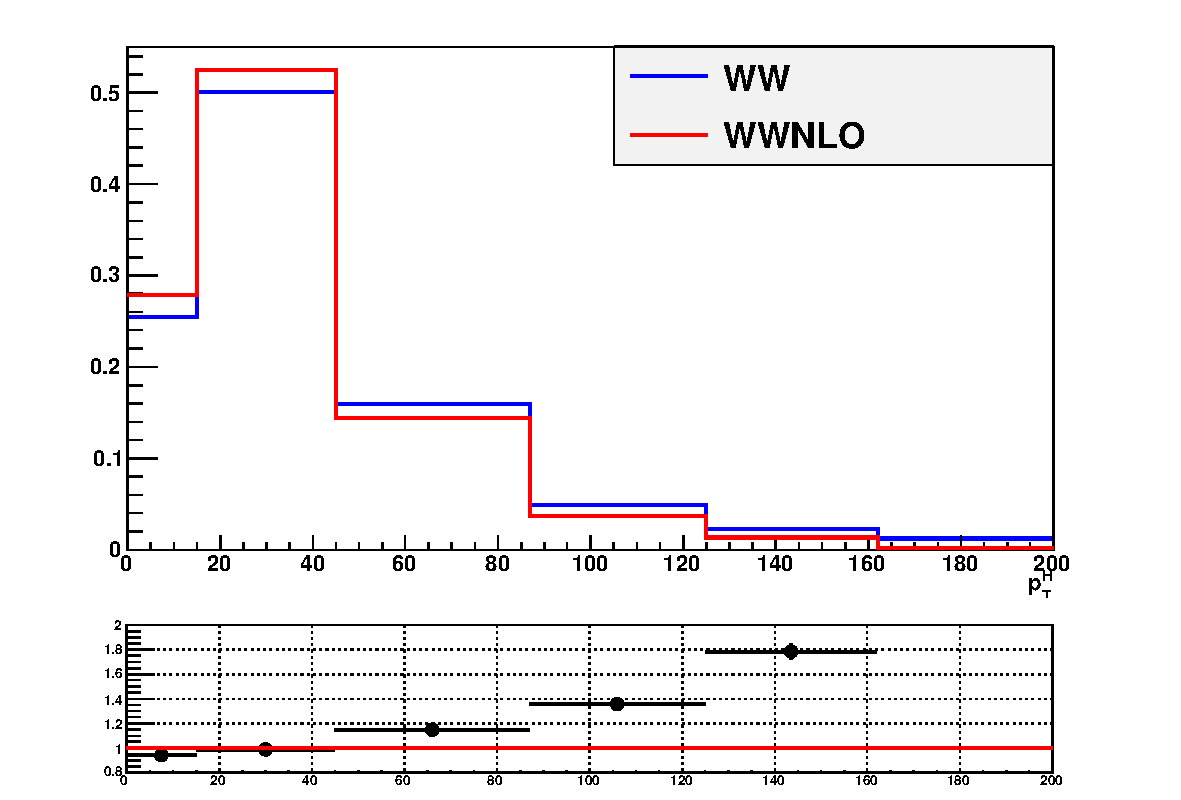
\includegraphics[width=0.7\textwidth]{images/WWnlo/WW_WWnlo.pdf}
\caption{Comparison between the $p_\mathrm{T}^\mathrm{WW}$ distributions obtained with two different MC generators: the blue line corresponds to the \textsc{Madgraph} generator and the red line refers to he same sample in which a reweighting has been applied in order to match the theoretical prediction at NLO+NNLL precision. }\label{fig:ww_wwnlo}
\end{figure}

A shape discrepancy can be clearly observed and the effect becomes larger at high values of \pth.
In order to assess the effect of this discrepancy on the shapes of the variables used for the signal extraction, \mll and \mt, the shapes have been checked in all \pth bins, comparing different MC samples. The \textsc{Madgraph} sample used for the nominal shape is compared to the \textsc{Madgraph} sample with NLO+NNLL  reweighting, a \textsc{Powheg} sample with NLO accuracy and an \textsc{aMC@NLO} sample.
The results of this comparison are shown in figures \ref{fig:ww_mll} and \ref{fig:ww_mth}. The shape discrepancy among the different models is included as an additional systematic uncertainty.

\begin{figure}[htb]
\centering
\subfigure[$0<\pth<15$\GeV]{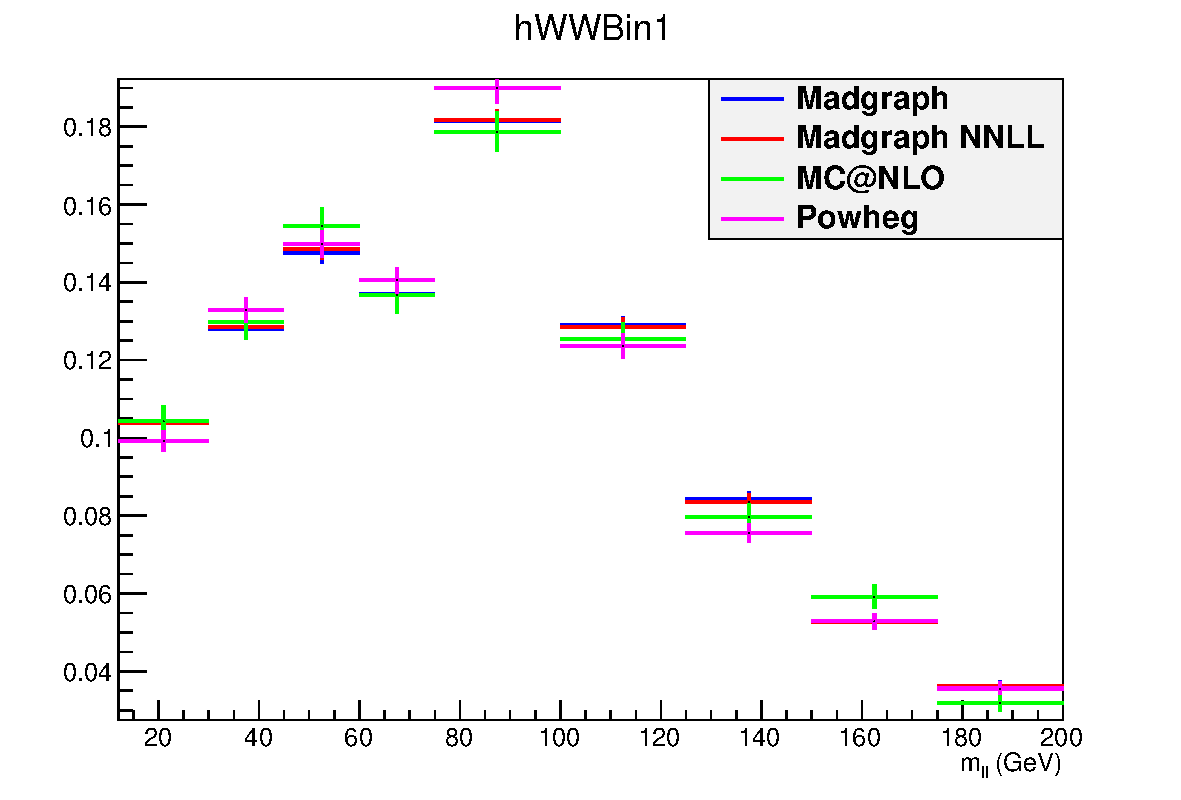
\includegraphics[width=0.45\textwidth]{images/WWnlo/mllBin1.pdf}}
\subfigure[$15<\pth<45$\GeV]{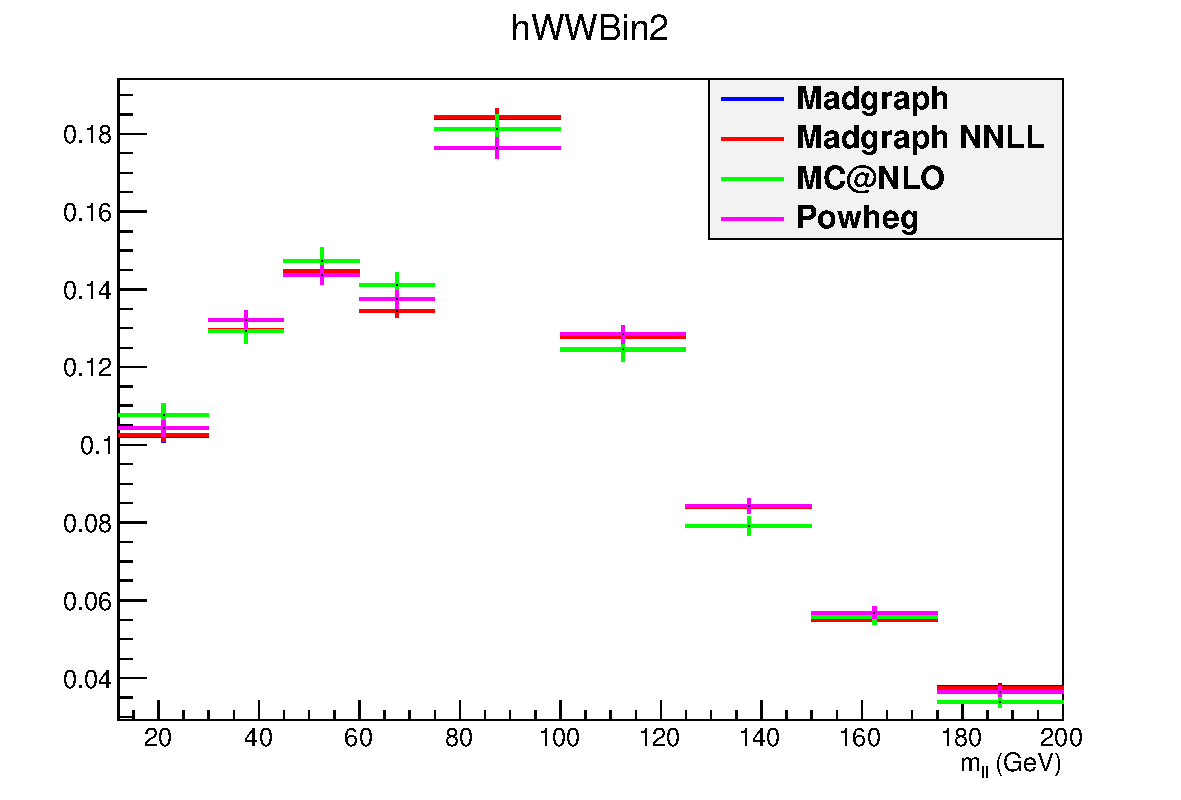
\includegraphics[width=0.45\textwidth]{images/WWnlo/mllBin2.pdf}}\\
\subfigure[$45<\pth<85$\GeV]{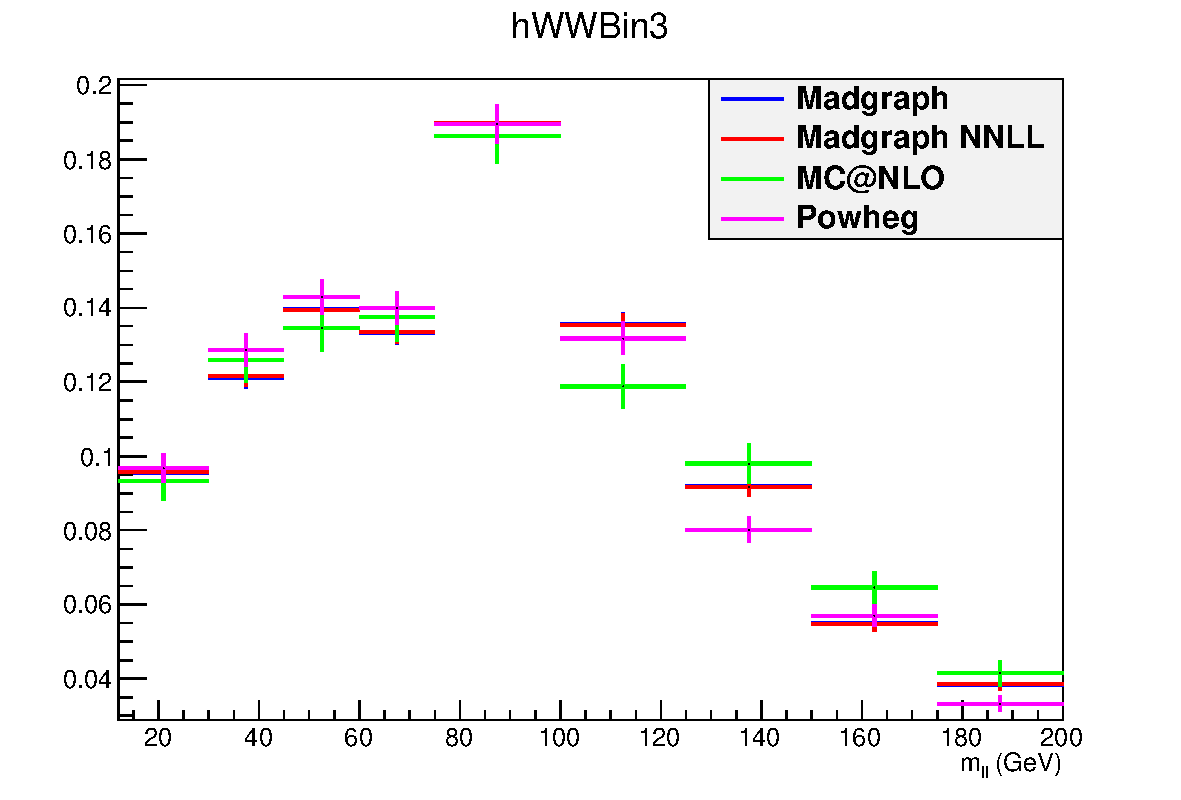
\includegraphics[width=0.45\textwidth]{images/WWnlo/mllBin3.pdf}}
\subfigure[$85<\pth<125$\GeV]{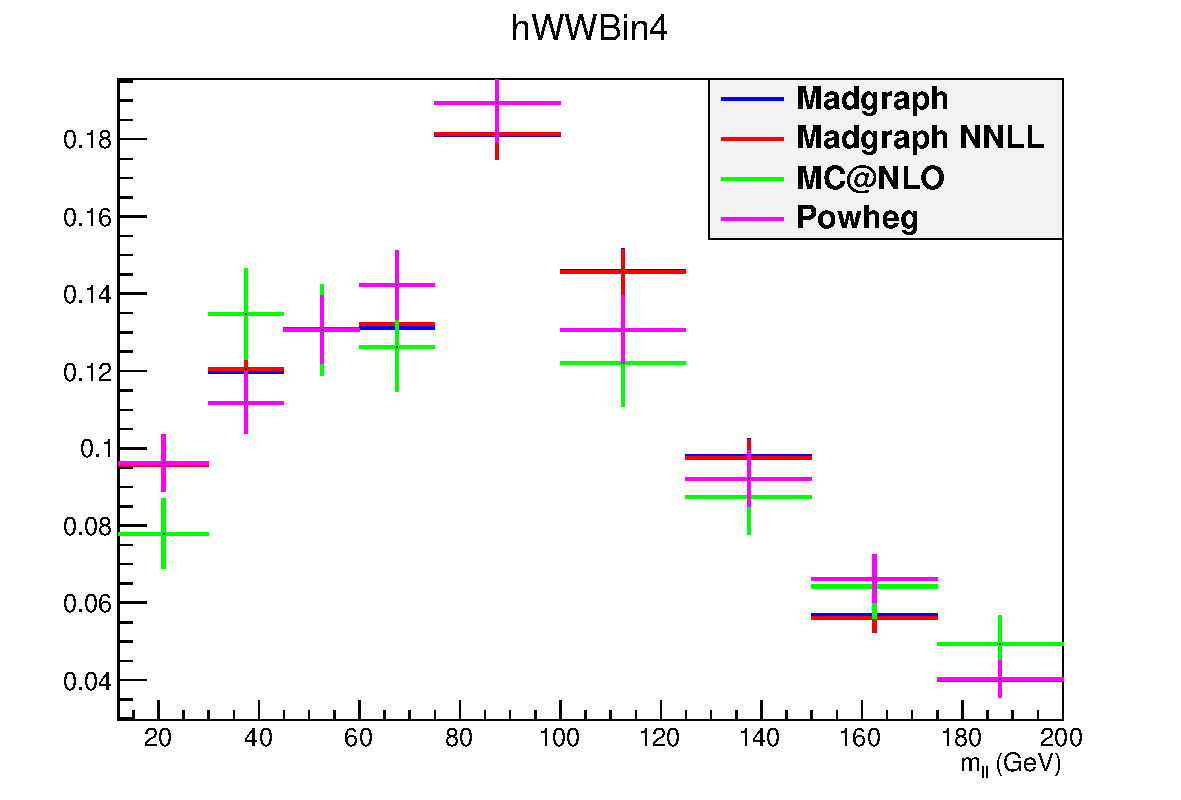
\includegraphics[width=0.45\textwidth]{images/WWnlo/mllBin4.pdf}}\\
\subfigure[$125<\pth<165$\GeV]{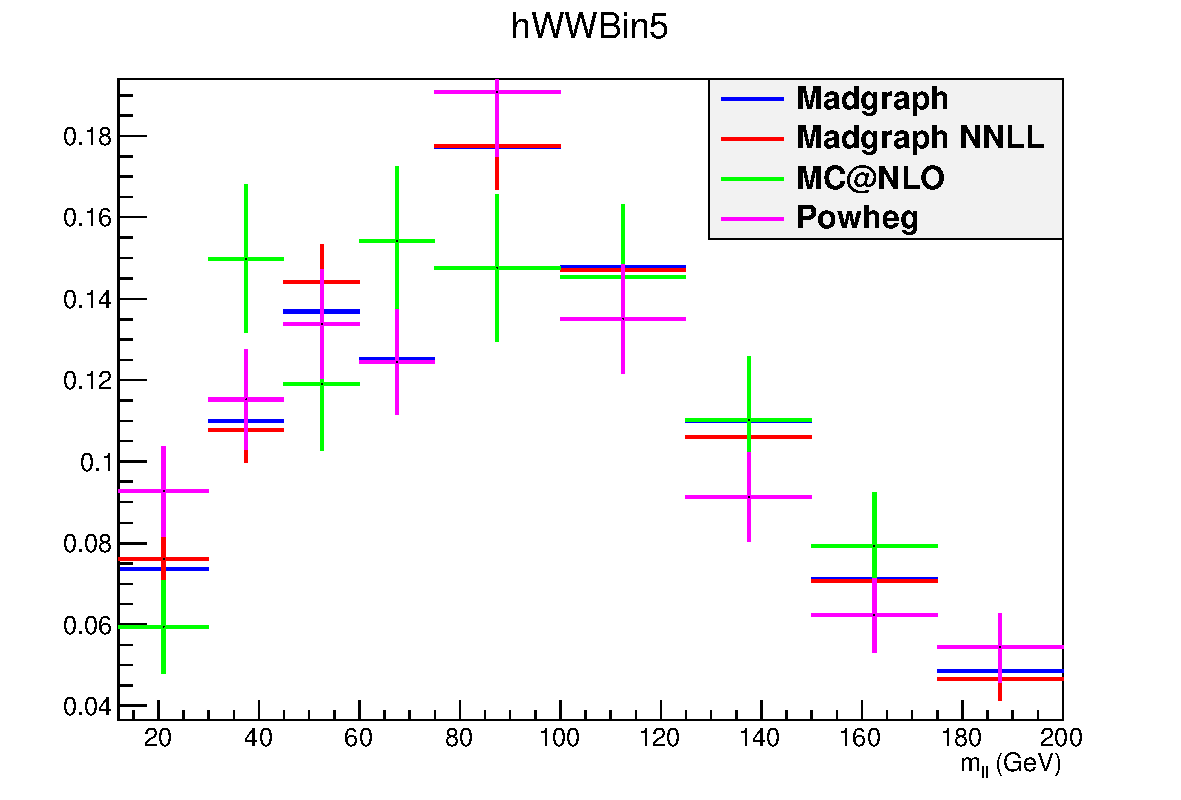
\includegraphics[width=0.45\textwidth]{images/WWnlo/mllBin5.pdf}}
\subfigure[$\pth>165$\GeV]{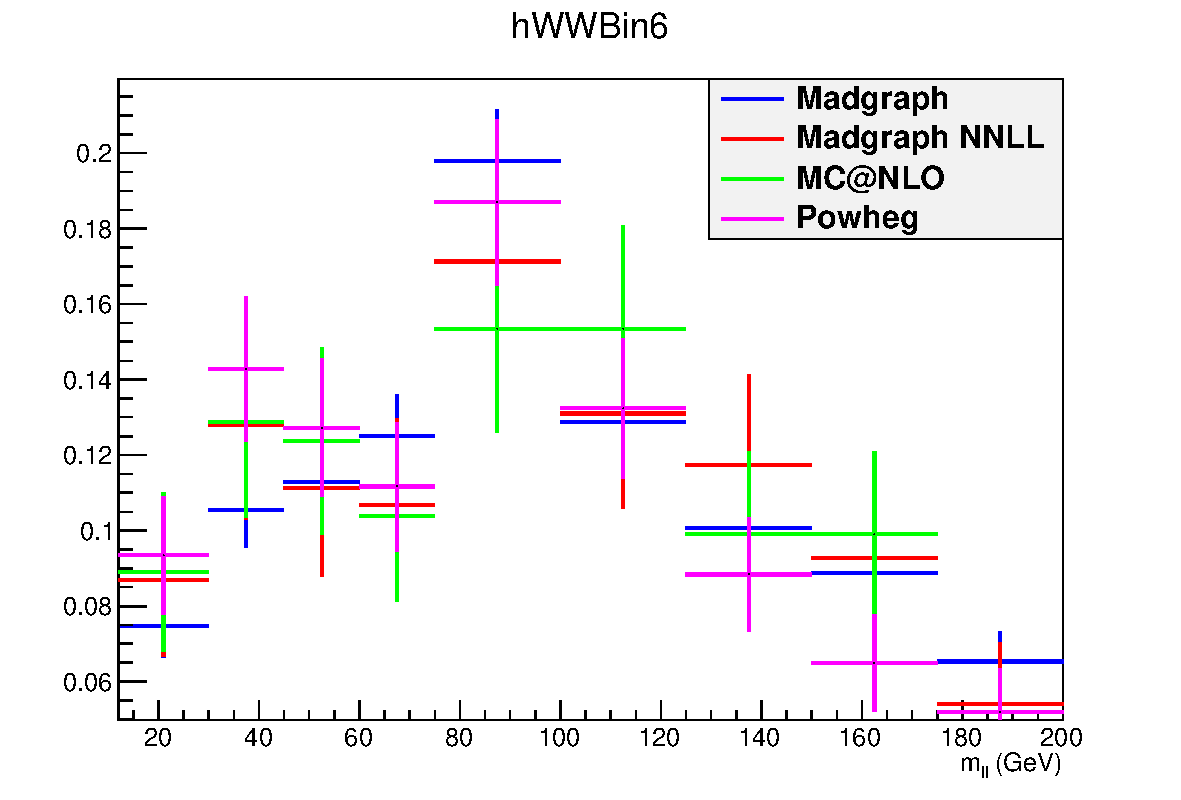
\includegraphics[width=0.45\textwidth]{images/WWnlo/mllBin6.pdf}}\\
\caption{Comparison between the default WW background sample and other theoretical models for the \mll distributions in every \pth bin.\label{fig:ww_mll}}
\end{figure}

\begin{figure}[htb]
\centering
\subfigure[$0<\pth<15$\GeV]{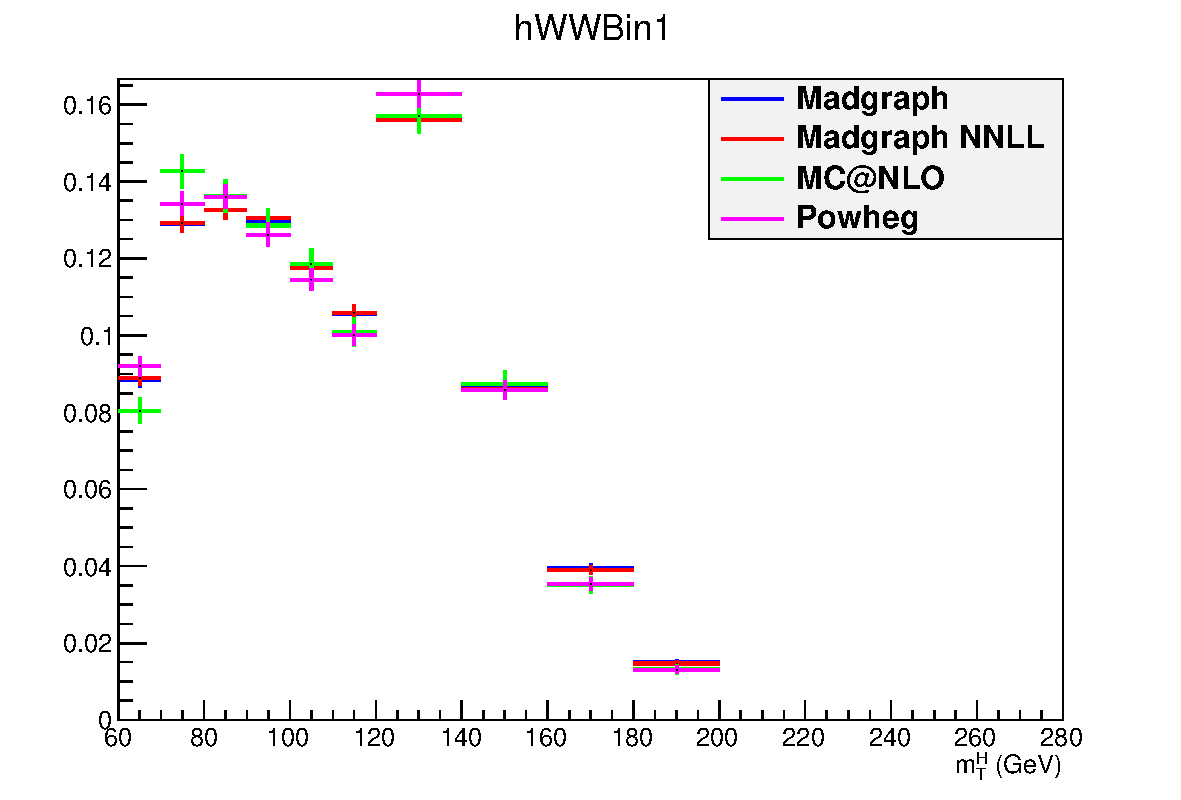
\includegraphics[width=0.45\textwidth]{images/WWnlo/mthBin1.pdf}}
\subfigure[$15<\pth<45$\GeV]{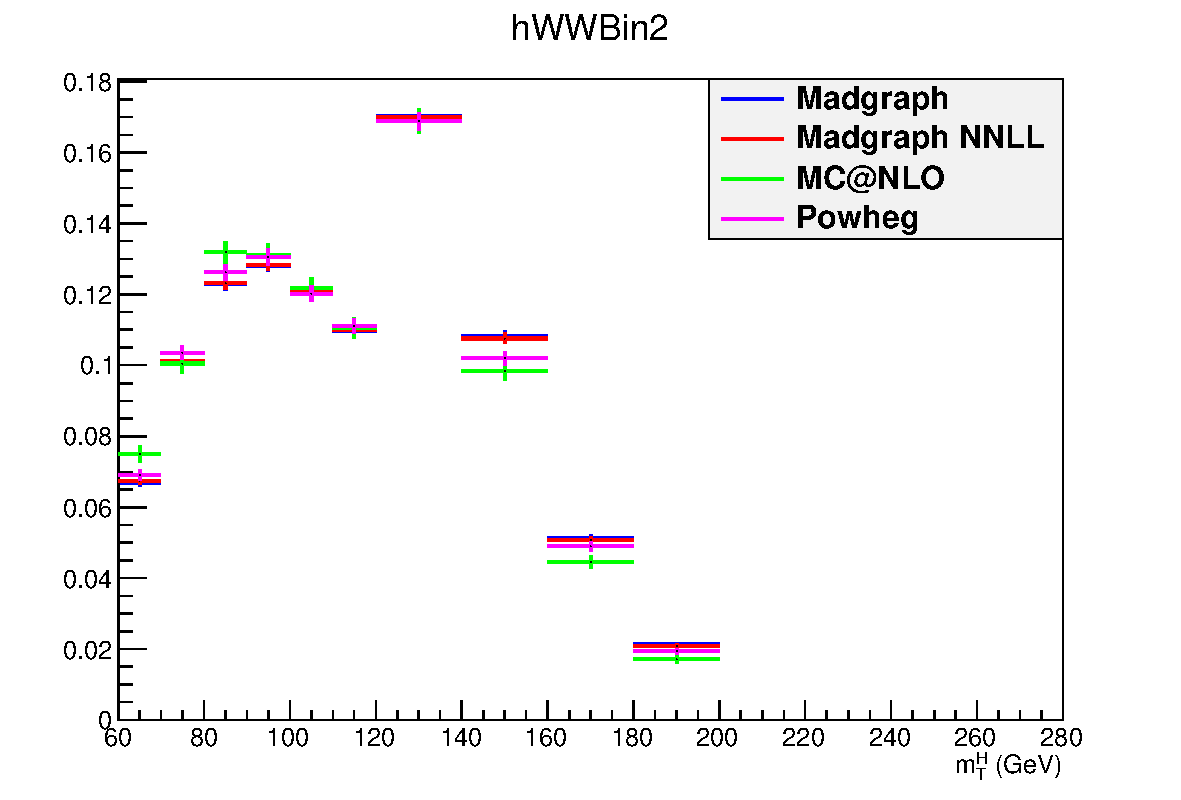
\includegraphics[width=0.45\textwidth]{images/WWnlo/mthBin2.pdf}}\\
\subfigure[$45<\pth<85$\GeV]{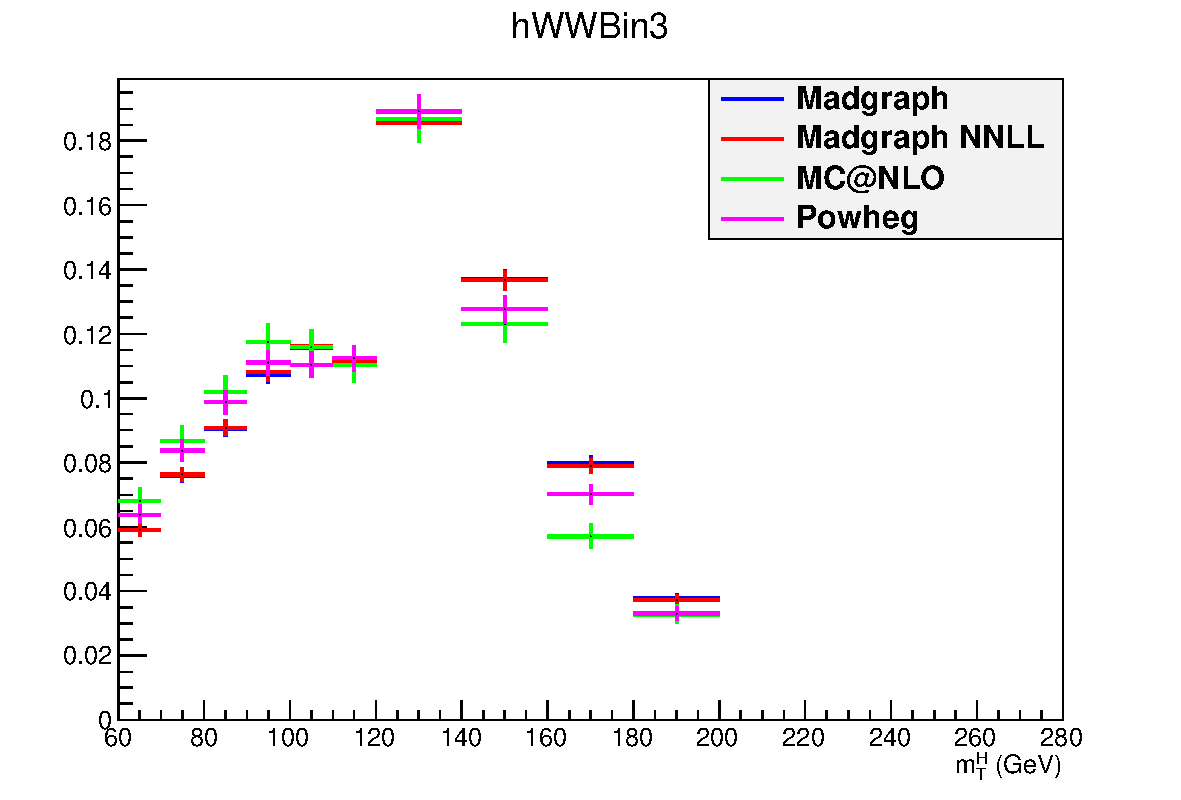
\includegraphics[width=0.45\textwidth]{images/WWnlo/mthBin3.pdf}}
\subfigure[$85<\pth<125$\GeV]{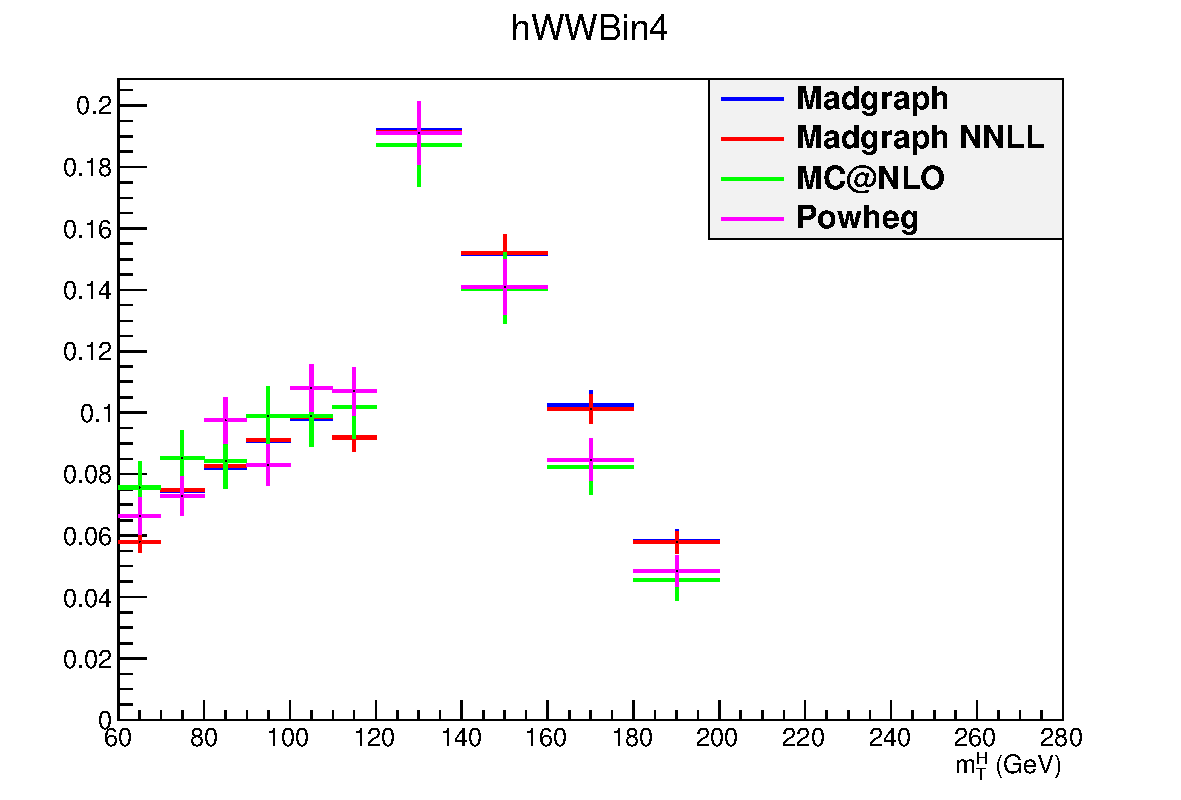
\includegraphics[width=0.45\textwidth]{images/WWnlo/mthBin4.pdf}}\\
\subfigure[$125<\pth<165$\GeV]{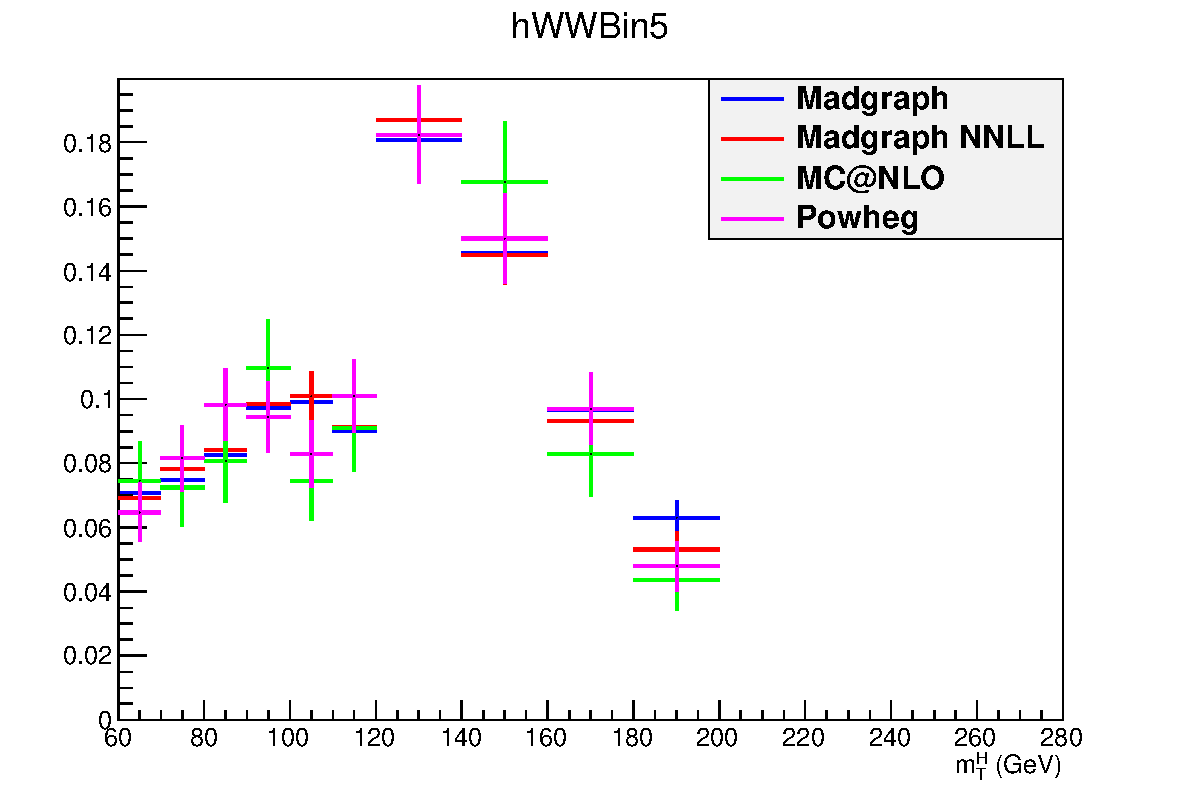
\includegraphics[width=0.45\textwidth]{images/WWnlo/mthBin5.pdf}}
\subfigure[$\pth>165$\GeV]{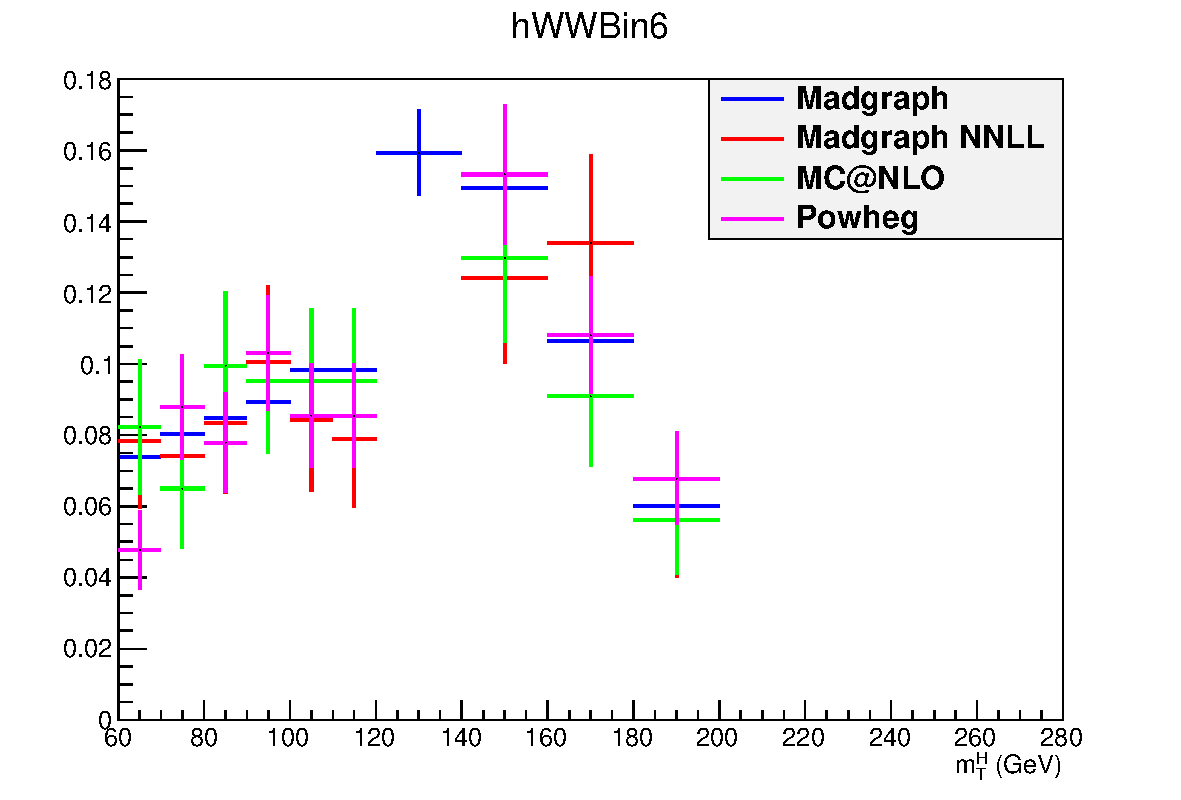
\includegraphics[width=0.45\textwidth]{images/WWnlo/mthBin6.pdf}}\\
\caption{Comparison between the default WW background sample and other theoretical models for the \mt distributions in every \pth bin.\label{fig:ww_mth}}
\end{figure}

The agreement of the \mll and \mt shapes between simulation and data for this background was checked in a signal-free control, defined selecting events with values of \mll greater than 60\GeV.

The gluon-induced WW process, i.e. gg$\to \mathrm{W^{+}W^{-}}$, has a sub-dominant contribution with respect to the quark-induced process, being the cross section ratio between the two of about 5\%. The \mll and \mt shapes for this background are taken from simulation while the cross section is scaled to the approximate NLO calculation~\cite{Bonvini:2013jha,Passarino:2013bha}.












































\subsection{Other backgrounds\label{sec:OtherBackgrounds}}

	%------------------------------------------------------------------------------------
	\subsubsection{Fake leptons background\label{sec:wjetsbkg}}	
	
Events in which W bosons are produced in association with jets, as well as multi-jet events, constitute a background for this analysis, because one or more jets can be misidentified as leptons. The rate at which jets are misidentified as leptons may be not accurately described in simulation, hence a data driven method is used to estimate this background. 
	
The idea is to estimate the background containing one or two fake leptons selecting events with relaxed lepton quality criteria, i.e. looser with respect to the selections used at the analysis level, and computing the efficiencies for real and fake leptons to pass the tight lepton quality requirements of the analysis. 
A data-driven approach is pursued to estimate this background. A set of loosely selected lepton-like objects, referred to as the ``fakeable object' or ``denominator'' from here on, is defined in a data set of events dominated by dijet production.
To measure the fake rate we count how many fakeable objects pass the full lepton selection 
of the analysis, parameterized as a function of the phase space of the fakeable lepton, therefore 
it is extracted in bins of $\eta$ and \pt.
The ratio of the fully identified lepton, referred as ``numerator'', to the 
fakeable objects is taken as the probability for a fakeable object to fake a lepton:

\begin{equation} \label{eq:fake_rate}
{Fake\ Rate } = \frac{\# of \ fully \ reconstructed \ leptons}{\# of \ fakeable \ objects} 
\end{equation}

It is then used to extrapolate from the loose leptons sample to a sample of leptons satisfying the  
full selection.

The definition of the denominator is of large impact in the systematic uncertainties related to this method. For the 2012 data taking period a summary of the selections used for the numerator and the denominator of Eq.~\eqref{eq:fake_rate} is shown below for electrons and muons respectively.
For electrons the denominator is defined by the following requirements:

\begin{itemize}
\item $\sigma_\mathrm{i\eta i\eta} < 0.01 (0.03)$ for barrel (endcap);
\item $|\Delta\phi_\mathrm{in}| < 0.15 (0.10)$ for barrel (endcap);
\item $|\Delta\eta_\mathrm{in}| < 0.007 (0.009)$ for barrel (endcap);
\item $H/E < 0.12 (0.10)$ for barrel (endcap);
\item electron conversion rejection;
\item $|d_0| < 0.02$\,cm;
\item $\frac{\sum_\mathrm{trk}E_\mathrm{T}}{\pt^\mathrm{ele}} < 0.2$;
\item $\frac{\sum_\mathrm{ECAL}E_\mathrm{T}}{\pt^\mathrm{ele}} < 0.2$;
\item $\frac{\sum_\mathrm{HCAL}E_\mathrm{T}}{\pt^\mathrm{ele}} < 0.2$.
\end{itemize}

For muons the selection are loosened with respect to the tight analysis selection requiring that:

\begin{itemize}
\item $|d_0| < 0.02$\,cm;
\item MVA isolation output $> -0.6$.
\end{itemize}

%shown in Table~\ref{tab:fake_muons} and \ref{tab_fake_electrons} for muons and electrons respectively.

%\begin{table}
%\centering
%\begin{tabular}{c c c}
%\hline
%Selection & Numerator & Denominator \\
%\hline\hline
%Muon ID & Global Muon + Tracker Muon & Tracker Muon \\
%\pt     & $\pt>20$\GeV & $\pt>20$\GeV \\
%$\eta$  & $|\eta|<2.4$ & $|\eta|<2.4$ \\
%Isolation & $(\mathrm{trackIso+caloIso})/\pt < 0.15$ & $(\mathrm{trackIso+caloIso})/\pt < 1$ \\
%\# inner tracker hits & $\mathrm{\# hits} > 10$ & $\mathrm{\# hits} > 10$ \\
%\# pixel hits & $\mathrm{\# hits} > 0$ & $\mathrm{\# hits} > 0$ \\
%Global $\chi^2$ & $\chi^2/\mathrm{ndof} < 10$ & -- \\
%$d0$ & $d0 < 0.02$\,cm & $d0 < 0.02$\,cm \\
%$dz$ & $dz < 1$\,cm & $dz < 1$\,cm \\
%\# valid SA hits & $>0$ & -- \\
%\# muon stations & $>1$ & -- \\
%\hline
%\end{tabular}
%\caption{Numerator and denominator selections for muons.\label{tab:fake_muons}}
%\end{table}

The dijet enriched data set used for the fake rate measurement, which is selected using single lepton triggers with low \pt thresholds, it is not a pure sample containing just fake leptons, but may still contain prompt leptons coming from the W and Z boson decays. To reject muons from the W decay, the events are required to have $\MET<20$\GeV and a W transverse mass below 20\GeV as well. Muons from the Z decay are instead remove requiring $m_{\mu\mu}>20$\GeV and $m_{\mu\mu} \notin [76,106]$\GeV. For electrons the Z mass peak veto is enlarged to $m_\mathrm{ee} \notin [60,120]$\GeV. Finally both electrons and muons are required to be isolated from the leading jet in the event, i.e. $\Delta\phi(\ell,j)>1$. The residual prompt lepton contamination from EW processes such as W/Z+jets production, which can bias the fake rate measurement, is estimated using simulation and subtracted from both the numerator and denominator. The contamination from EW processes is different for the numerator and denominator and is particularly important for relatively high lepton \pt values.

In addition to the fake rate, also a prompt lepton rate is evaluated, defined as the probability of a prompt lepton passing the loose requirements to also pass the tight analysis selections.
The prompt rate is also measured in data, defining a control region enriched in $\mathrm{Z} \to \ell\ell$ events, selecting dilepton events with an invariant mass of the two leptons in the Z peak mass region.

Both the fake and prompt rate are used to reweight the data samples used in the analysis in order to obtain directly from data the contribution of the fake lepton background. The method to apply those rates is explained below in the simple case of just one lepton in the data sample, i.e. data selected by single lepton triggers, but can be straightforwardly generalized to more complex situations.
Suppose that the total number of leptons passing the loose requirements, $N_\ell$, is made up of $N_p$ prompt and $N_f$ fake leptons. $N_p$ and $N_f$ cannot be directly measured but one can measure the number of events where no leptons, $N_{t0}$, or one lepton, $N_{t1}$, pass the tight analysis requirement. These numbers are related by the following equations:

\begin{equation}\label{eq:fake_single_lep}
\begin{gathered}
    N_\ell = N_p + N_f = N_{t0} + N_{t1}\\
    N_{t0} = (1-p)N_p + (1-f)N_f\\
    N_{t1} = pN_p + fN_f
\end{gathered}
\end{equation}

where $p$ and $f$ are the prompt and fake rates respectively. Equation~\eqref{eq:fake_single_lep} can be inverted to obtain the number of prompt and fake leptons:

\begin{equation}\label{eq:fake_prompt}
\begin{gathered}
    N_p = \frac{1}{p-f}\left[ (1-f)N_{t1} - fN_{t0}  \right]\\
    N_f = \frac{1}{p-f}\left[ pN_{t0} - (1-p)N_{t1}  \right]\\
\end{gathered}
\end{equation}

The systematic uncertainty is evaluated by varying the jet thresholds in the di-jet control sample, and by
performing a closure test in the same-sign data sample (see~\cite{AN-2013-022}) \textcolor{red}{REFERENZE}. In both cases it is about 36\%.

	%-------------------------------------------------------------------------------
	\subsubsection{Drell-Yan to \texorpdfstring{$\tau\tau$}{tau tau} background\label{sec:DYtautaubkg}}


The low \MET threshold in e$\mu$ final state
requires the consideration of the contribution from 
\dytt\, that is in fact estimated from data.
This is accomplished by using 
\dymm events and replacing muons with a simulated
$\tau\to l\nu_\tau\bar{\nu_e}$ decay \cite{AN-2011-020} \textcolor{red}{REFERENZE}.\\
After replacing muons from \dymm decays with simulated $\tau$ decays,
the set of pseudo \dytt events undergoes the reconstruction step.
 
Good agreement in kinematic distributions for this sample
and a MC based \dytt sample is found.
The global normalization of pseudo \dytt events is 
checked in the low \mt spectrum where a rather pure
\dytt sample is expected.


	%-------------------------------------------------------------------------------
	\subsubsection{ZZ, WZ and W\texorpdfstring{$\gamma$}{gamma} backgrounds\label{sec:otherbkg}}

The WZ and ZZ backgrounds are partially estimated from data when the two
selected leptons come from the same Z boson. If the leptons come from different
bosons the contribution is expected to be small. The WZ component is largely
rejected by requiring only two high \pt isolated leptons in the event. 
%The missing energy requirement makes the ZZ~$\to 4\ell$ component almost negligible.
%As the extra lepton veto and the \met cuts do not remove the ZZ~$\to 2\ell 2\nu$
%decays, a non-negligible fraction of these events survives the selection for $ee$ and $\mu\mu$ channels only. 

The W+$\gamma^{(*)}$ background, where the photon decays to an electron-positron pair,
is expected to be very small, thanks to the stringent photon conversion
requirements.
 Since the WZ simulated sample has a generation level cut on the
di-lepton invariant mass ($m_{\ell\ell} >$ 12~\GeV) and the cross-section raises
quickly with the lowering of this threshold, a dedicated \textsc{Madgraph} sample has
been produced with lower momentum cuts on two of the three leptons
($\pt > 5$~\GeV) and no cut on the third one. The surviving contribution
estimated with this sample is still very small, and since the uncertainty on the
cross-section for the covered phase space is large, a conservative 100\%
uncertainty has been given to it. 
A $k$-factor for W+$\gamma^{*}$ of $1.5\pm0.5$ based on a dedicated measurement of 
tri-lepton decays, W+$\gamma^{*} \to e\mu\mu$ and W+$\gamma^{*} \to \mu\mu\mu$,
is applied~\cite{WGammaStarStudy} \textcolor{red}{REFERENZE}. 
The contribution of W+$\gamma^{(*)}$ is also
constrained by a closure test with same sign leptons on data, which reveals a
good compatibility of the data with the expected background.


%\clearpage
\section{Systematic uncertainties}
%%%%%%%%%%%%%%%%%%%%%%%%%%%%%%%%%%%%%%%%%%%%%%%%%%%%%%%%%%%%%%%%%%%%%%
\label{sec:Systematics}

Systematic uncertainties play an important role in this analysis where
no strong mass peak is expected due to the presence of undetected
neutrinos in the final state. They arise from three sources: background predictions, experimental measurements, and theoretical uncertainties. One of the most important sources is the normalization of the backgrounds that are estimated on data control samples whenever is possible.

The systematic uncertainties can affect the measured signal strengths in different ways. The uncertainties on the background predictions can be divided in those affecting the background cross section, the (\mll, \mt) shape or both. As an example, systematic uncertainties changing the background cross section are the ones related to the background data-driven estimation, while the b tagging uncertainties only have an effect on the (\mll, \mt) shape. Uncertainties such as lepton energy scale can instead affect both normalization and shape. Also, uncertainties affecting the signal (\mll, \mt) shape reflect on an uncertainty on the measured signal strength. 

A summary of the main sources of systematic uncertainty and the corresponding estimate is reported in Table~\ref{tab:Systematics}. A brief description of each source of systematic uncertainty is discussed in the following sections.

The uncertainties related to the unfolding procedure are treated separately and are discussed in Sec.~\ref{sec:uncunf}.

\begin{table}[h]
\small{
  \begin{center}
  \caption{Main sources of systematic uncertainties and their estimate. The
  first category reports the uncertainties on the normalization of background
  contributions. The experimental and theoretical uncertainties refer to the
  effect on signal yields. A range is specified if the uncertainty varies
  across the $\pth$ bins.}
  \label{tab:Systematics}
  \begin{tabular}{cc}
  \hline\hline
  \multicolumn{2}{c} {\bf{Uncertainties in backgrounds contributions}} \\
  \hline
  Source  & Uncertainty \\
  \hline
  $\rm{t\bar{t}}$, tW      & 20--50$\%$ \\
  W+jets              & $40\%$ \\
  WZ, ZZ              & $4\%$ \\
  W$\gamma^{*}$, W$\gamma$  & $30\%$ \\
  \hline\hline
  \multicolumn{2}{c} {\bf{Effect of the experimental uncertainties on the signal and background yields}}\\
  \hline
  Source & Uncertainty\\
  \hline
  Integrated luminosity        & $2.6\%$ \\
  Trigger efficiency           & 1--2$\%$\\
  Lepton reconstruction and identification & 3--4$\%$\\
  Lepton energy scale          & 2--4$\%$ \\
  \MET modelling          & $2\%$ \\
  Jet energy scale             & $10\%$ \\
  Pileup multiplicity          & $2\%$ \\
  b mistag modelling	       & $3\%$ \\	
  \hline\hline
  \multicolumn{2}{c}{\bf{Effect of the theoretical uncertainties on signal yield}}\\
  \hline
  Source & Uncertainty \\
  \hline
  b jet veto scale factor              & 1--2$\%$\\
  PDF                                  & $1\%$ \\
  WW background shape                  & $1\%$\\
  \hline
  \end{tabular}
  \end{center}
}
\end{table}


%-------------------------------------------------------------------------------
\subsection{Background predictions uncertainties}
%-------------------------------------------------------------------------------

The signal extraction is performed fitting the estimated background contributions and subtracting them to the event counts in data. Therefore, the uncertainties on the background predictions indirectly reflect as uncertainties on the signal measurements. A list of the most important background uncertainties is given below.

\begin{itemize}
\item {\bf\boldmath \ttbar and tW backgrounds:}    
the shapes of these backgrounds are corrected for different b tagging efficiency in data and simulation, and the normalization is taken from data in a top quark enriched control region independently in each \pth bin, as explained in Sec.~\ref{sec:TTBackground}. The uncertainties related to this procedure arise from the sample size in the control regions for each \pth bin, and are embedded in the $\alpha$ factors used to extrapolate
the top quark background normalization from the control region to the signal region. They vary from 20\% to 50\% depending on the \pth bin.
   
The simulated samples include both \ttbar and tW processes, a systematic uncertainty related to the tW$/$\ttbar fraction has been included.
In fact, a relative variation of the contribution of these two processes could modify the shape of the simulated sample, and is thus included as a shape uncertainty affecting the (\mll, \mt) shape in each \pth bin in a correlated way. 

\item {\bf \boldmath{WW background}:} 
due to the fact that the WW background (\mll, \mt) shape is entirely taken from simulation, the analysis is relying on theoretical models and can thus be affected by their uncertainties. Especially higher order QCD radiative effects have an influence on the generated WW shape. To study this impact, the shapes of the distributions produced with the \textsc{MadGraph} generator are compared to the ones produced with \textsc{mc@nlo} and other generators (see Sec.~\ref{sec:WWBackground}). The comparison is performed separately in each bin of \pth and the uncertainty includes shape differences originating from the renormalization and factorization scale choice. The effect on the signal strengths is found to be of the order of 1\%.
  
\item {\bf\boldmath W+jets background:} 
the systematic uncertainties on the W+jets background arise from the estimation method explained in Sec.~\ref{sec:wjetsbkg}. This uncertainty has two sources: the dependence of $\varepsilon_\mathrm{pass}$ on the sample composition, and the method. The first source is estimated by modifying the jet \pt threshold in the QCD multijet sample, which modifies the jet sample composition.  The uncertainty in the method is obtained from a closure test, where $\varepsilon_\mathrm{pass}$ is derived from simulated QCD multijet events and applied to simulated samples to predict the number of background events. The total uncertainty in $\varepsilon_\mathrm{pass}$, including the statistical precision of the control sample, is of the order of 40\%.
 
\item {\bf\boldmath Diboson backgrounds:} 
these backgrounds are expected to give a small contribution in the signal phase space. Uncertainties on the cross sections reported in \cite{xsecSM,bib:ellis} are 4\% for WZ and 2.5\% for ZZ. A 30\% uncertainty is assigned to the $W\gamma$ \cite{WgammaXsec} yield and another 30\% on $W\gamma^{*}$ contribution according to the uncertainty on the normalization study (see Sec.~\ref{sec:diboson}).
      
\end{itemize}

%-------------------------------------------------------------------------------
\subsection{Experimental uncertainties \label{subsec:expsyst}}
%-------------------------------------------------------------------------------

The following experimental systematic sources have been taken into account:

\begin{itemize}
\item {\bf Luminosity:} using the CMS online luminosity monitoring system, the uncertainty on the integrated luminosity (19.4\ifb) collected during the 2012 data taking period is found to be of $2.6\%$.

\item {\bf Trigger efficiency:} the uncertainties for both electrons and muons, estimated as described in Sec.~\ref{sec:trigeff}, are at 1-2\% level.

\item {\bf Lepton reconstruction and identification efficiency:} 
this uncertainty is estimated with the Tag and Probe technique described in Sec.~\ref{sec:leptonID}, resulting in a 4\% uncertainty for electrons and 3\% for muons.

\item {\bf Muon momentum and electron energy scale:} 
the momentum scale of leptons has relatively large uncertainties due to different detector effects, as explained in Sec.~\ref{sec:leptonID}. For electrons a scale  uncertainty of 2\% for the barrel, and 4\% for the endcaps respectively, is assigned. For muons, a momentum scale uncertainty of 1.5\%, independent on the muon pseudorapidity, is assigned.

\item {\bf {\boldmath \MET} modelling:} 
  the \MET measurement is affected by the possible mis-measurement of 
  individual particles addressed above, as well as the additional contributions 
  from the pile-up interactions, as described in Sec.~\ref{sec:met}. 
  The effect of the missing transverse momentum resolution on the event selection
  is studied by applying a Gaussian smearing of 10\% on the $x$- and
  $y$-components of the missing transverse momentum. All correlated variables,
  like the transverse mass, are recalculated. The effect is found to be around 2\%.

\item {\bf Jet energy scale (JES) uncertainties:} 
  JES uncertainties affect both the jet multiplicity and the jet kinematic variables, reflecting also on the (\mll, \mt) shape.
  This uncertainty is estimated varying the kinematics of the reconstructed jets within the uncertainties on the JES (which depend on $\eta$ and $\pt$ of the jet) described in Sec.~\ref{sec:jets}, and recomputing all the correlated variables, like \mll and \mt.

\item {\bf b-jets misidentification modelling:}
a fraction of signal events is rejected because erroneously identified as b-jets by the b tagging algorithms. The misidentification probability, as measured with the Tag and Probe technique described in Sec.~\ref{sec:ScaleFactors}, has an uncertainty related to different b tagging performance in data and simulation. This affects also non-top quark backgrounds.
          
\item {\bf Pileup multiplicity:} 
some of the variables used in the analysis are affected by the average number of pile up interactions. The simulated events have been reweighted according to the instantaneous luminosity measured on data. The error on the average number of pile up interactions measured in data and the simulation of the modelling and physics aspects of the pile up simulation provide an uncertainty of at most 5\% on the distribution used in the reweighting procedure. This uncertainty is propagated through all the analysis, and the estimated uncertainty on the signal strengths do not exceed 2\%.

\end{itemize}

%-------------------------------------------------------------------------------
\subsection{Theoretical uncertainties \label{subsec:thsyst}}
%-------------------------------------------------------------------------------

Theoretical uncertainties generally arise from missing higher-order corrections in QCD and PDF uncertainties. These uncertainties can affect both the cross section and the (\mll, \mt) shape of the background predictions, as well as the shape of the signal model.

\begin{itemize}

\item {\bf QCD scale uncertainties:}
the uncertainties on the total cross sections due to the choice of the renormalization and factorization scale are assigned to simulation-driven backgrounds. For the signal processes these uncertainties are separated in two categories: those affecting the selection efficiency and those affecting the jet bin fractions. The effect of renormalization and factorization scale on the selection efficiency is of the order of 2\% for all processes. Although this analysis is inclusive in number of jets, the effect of the QCD scales variation on the jet bin migrations has to be taken into account because of the b tagging veto efficiency. Indeed, the b tagging veto efficiency is not flat as a function of jet multiplicity not \pth, as shown in Fig.~\ref{fig:bveto_eff}, therefore introducing a dependence of the selection efficiency on the number of jets on the event.
In order to take into account this effect, an uncertainty on the ggH production mode has been included according to the Stewart-Tackman method, following the recipe proposed in Refs.~\cite{Stewart:2011cf,Heinemeyer:2013tqa}. The effect on the signal strengths is found to be of the order of 1--2\%.

\item {\bf PDFs uncertainties:} 
the utilization of different PDF sets can affect the (\mll, \mt) shapes of the signal contributions, as well as the normalization and shape of the background predictions. The uncertainty related due to the variations in the choice of PDFs is considered following the PDF4LHC~\cite{Alekhin:2011sk,Botje:2011sn} prescription, using CT10, NNPDF2.1~\cite{Ball:2011mu} and MSTW2008~\cite{Martin:2009iq} PDF sets. The effect on the signal strengths is found to be of at most 1\%.

\end{itemize} 

\begin{comment}
\subsubsection{Jet multiplicity uncertainty} \label{subsec:stewart-tackman}

The jet bin uncertainty on the ggH production mode has been evaluated using the Stewart-Tackman method, following the recipe proposed in Refs.~\cite{Stewart:2011cf,Heinemeyer:2013tqa}.
Three independent nuisance parameters have to be associated with the inclusive ggH production cross sections $\sigma_{\geq 0}$, $\sigma_{\geq 1}$ and $\sigma_{\geq 2}$, which corresponds to the cross sections with $\geq 0$ jets, $\geq 1$ jet and $\geq 2$ jets respectively. According to the agreement on the treatment of uncertainties in the combination of ATLAS and CMS results~\cite{ATLAS:2011tau}, these nuisance parameters are labelled as \emph{QCDscale\_ggH}, \emph{QCDscale\_ggH1in} and \emph{QCDscale\_ggH2in}. However, in case the analysis is split in exclusive jet multiplicity bins, the jet bin uncertainties can be evaluated taking into account the correct correlations among the three nuisances following the Stewart-Tackman prescription.
Even though this analysis is inclusive in number of jets, the jet binning uncertainties must be included due to the presence of the b-jet veto, that introduces a dependency of the selection efficiency on the number of jets in the event. The veto efficiency has been evaluated in all the \pth bins defined in the analysis and as a function of jets multiplicity. The results are shown in Figs.~\ref{fig:veto_eff_pth} and \ref{fig:veto_eff_njet}. The drop of the veto efficiency at high values of \pth is due to the correlation with jets multiplicity.
	 	
\begin{figure}[htb]
\centering
	\subfigure[]{
		\centering
		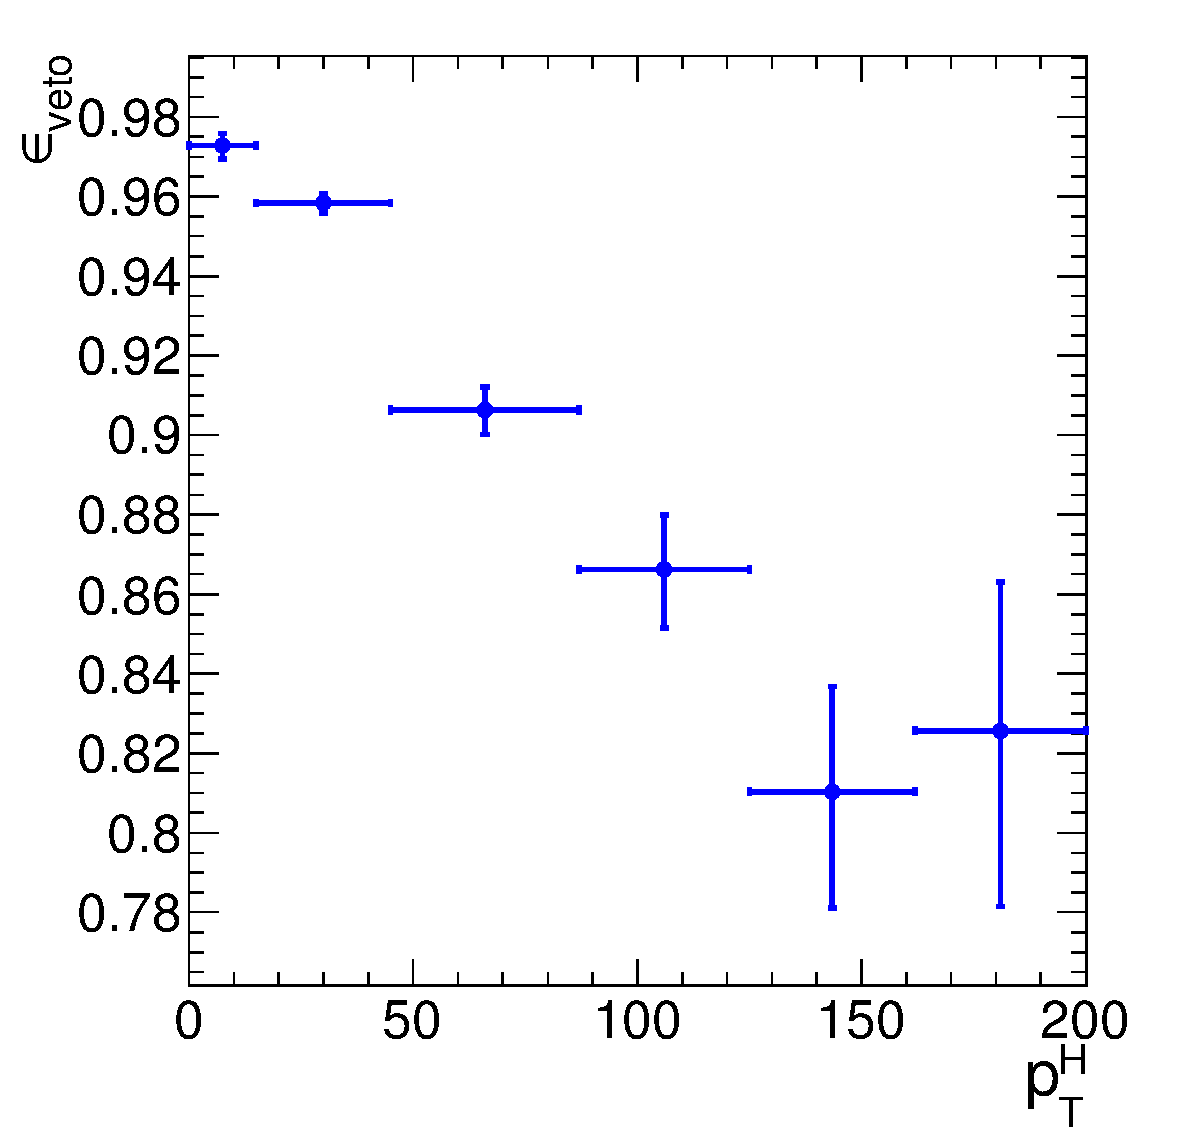
\includegraphics[width=0.45\textwidth]{images/eff_vs_pth.pdf}
		\label{fig:veto_eff_pth}
	}
	\subfigure[]{
		\centering
		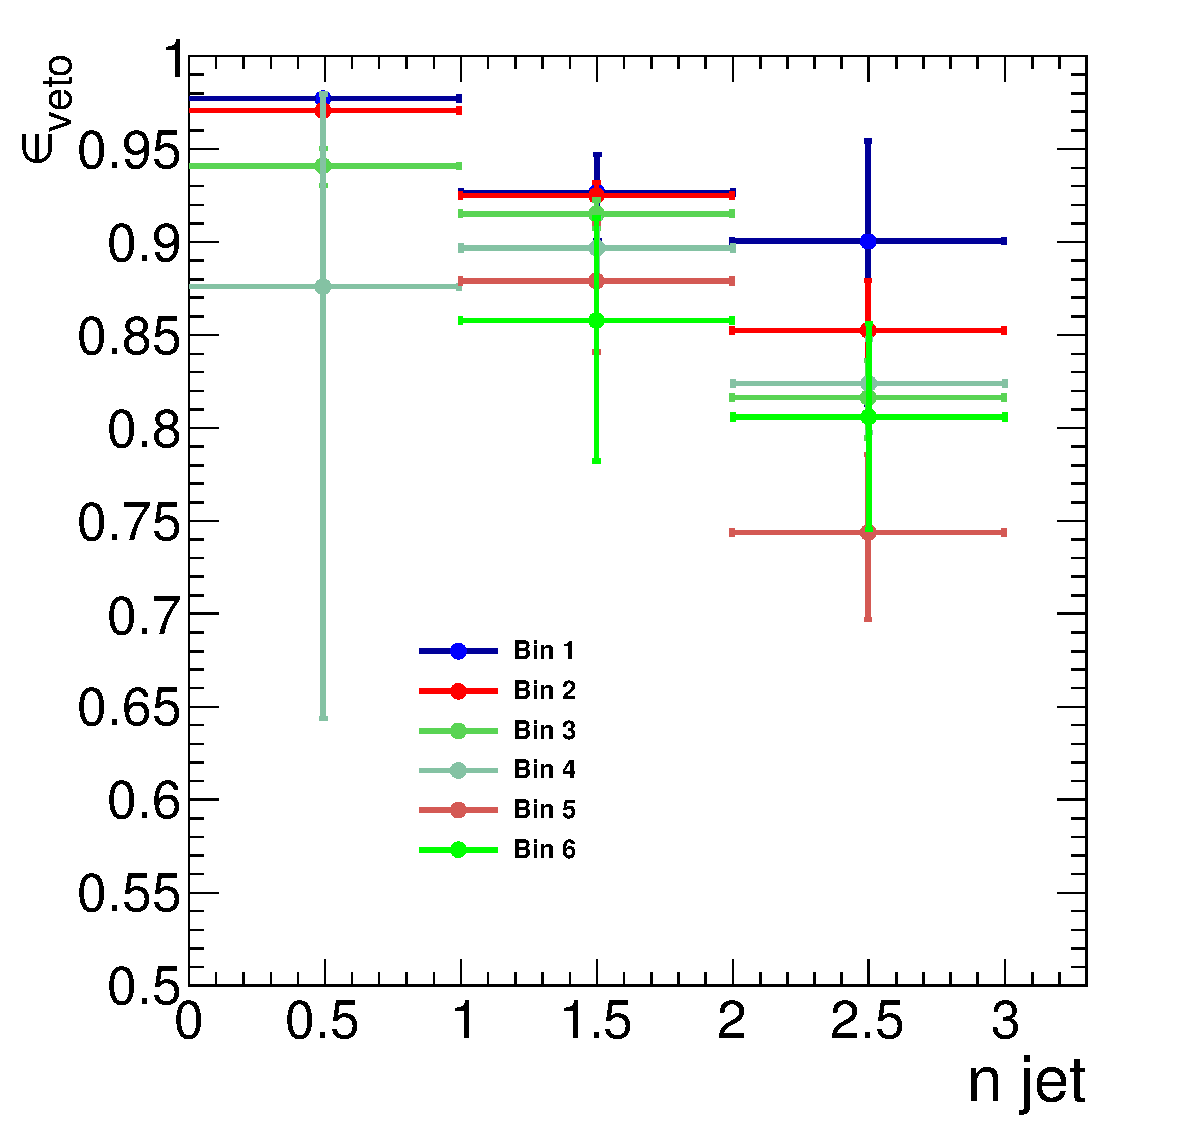
\includegraphics[width=0.45\textwidth]{images/eff_vs_jet.pdf}
		\label{fig:veto_eff_njet}
	}
\caption{(a) Efficiency of the b-tagging veto in different bins of \pth. (b) Efficiency of the b-tagging veto in different bins of \pth, as a function of number of jets.}\label{fig:bveto_eff}
\end{figure}

The first step of this procedure is to take the inclusive ggH cross section, $\sigma_\mathrm{ggH}$, and to convert the relative QCD up/down scale uncertainties, $\epsilon_+$ and $\epsilon_-$, to a log-normal uncertainty, i.e. $\kappa = \sqrt{\exp{(\epsilon_+)}\cdot \exp{(\epsilon_-)}}$. The exclusive cross sections, $\sigma_0$, $\sigma_1$ and $\sigma_2$, can be calculated starting from $\sigma_\mathrm{ggH}$ and using the selection efficiencies for the three jet bins. For every exclusive cross section the corresponding relative uncertainty is computed varying the renormalization ($\mu_R$) and factorization ($\mu_F$) scales independently of a factor 2 and $1/2$, and taking the cross section value corresponding to half of the maximum variation. The inclusive cross sections are then obtained summing the exclusive cross sections and propagating the uncertainties, i.e. $\sigma_{\geq 0 } = \sigma_0 + \sigma_1 + \sigma_2$, $\sigma_{\geq 1} = \sigma_1 + \sigma_2$, $\sigma_{\geq 2} = \sigma_2$.

The three nuisance parameters, including all the proper correlations among the jet bins, are defined according to Table~\ref{table:jet_binning_theory}, where the $f_n$ constants represent the exclusive theoretical $n$ jet bin fractions, i.e. $f_0 = \sigma_0/\sigma_{\geq 0}$, $f_1 = \sigma_1/\sigma_{\geq 0}$, $f_2 = \sigma_2/\sigma_{\geq 0}$.

\begin{table}[h]
\caption{Numerical calculation for the systematic uncertainties of jet binning.}
\label{table:jet_binning_theory}
\begin{center}
\begin{tabular}{|l|c|c|c|}
\hline
Nuisance parameter & 0-jet bin                                              & 1-jet bin                                            & 2-jet bin \\ 
\hline
&&& \\
QCDscale\_ggH          & $\Delta^0_{\geq 0} = (\kappa_{\ge 0})^{\frac{1}{f_0}} $    &      & \\ 
&&&\\\hline
&&&\\
QCDscale\_ggH1in       & $\Delta^0_{\geq 1} = (\kappa_{\ge 1})^{- \frac{f_1 + f_2}{f_0}} $ & $\Delta^1_{\geq 1} = (\kappa_{\ge 1})^{\frac{f_1 + f_2}{f_1}} $ & \\ 
&&&\\ \hline
&&&\\
QCDscale\_ggH2in        &                                                        & $\Delta^1_{\geq 2} = (\kappa_{\ge 2})^{- \frac{f_2}{f_1}} $     & $\Delta^2_{\geq 2} = (\kappa_{\ge 2})$ \\ 
&&&\\\hline

\end{tabular}
\end{center}
\end{table}

The nuisance parameters reported in table \ref{table:jet_binning_theory} have then been calculated for each \pth bin embedding the b-jet veto efficiency and using the following formulas:
\begin{equation}
\emph{QCDscale\_ggH}=\frac{\Delta^0_{\geq 0}\cdot f_{0}\cdot \varepsilon_{0}+\Delta^0_{\geq 1}\cdot f_{1}\cdot\varepsilon_{1}}{\Delta^0_{\geq 0}\cdot f_{0}\cdot \varepsilon_{0}+\Delta^0_{\geq 1}\cdot f_{1}\cdot \varepsilon_{0}} \quad,
\end{equation}
\begin{equation}
\emph{QCDscale\_ggH1in}=\frac{\Delta^1_{\geq 1}\cdot f_{1}\cdot \varepsilon_{1}+\Delta^1_{\geq 2}\cdot f_{2}\cdot \varepsilon_{2}}{\Delta^1_{\geq 1}\cdot f_{1} \cdot \varepsilon_{1}+\Delta^1_{\geq 2}\cdot f_{2}\cdot \varepsilon_{1}} \quad,
\end{equation}
\begin{equation}
QCDscale\_ggH2in=1 \quad,
\end{equation}
where $\varepsilon_0$, $\varepsilon_1$ and $\varepsilon_2$ are the selection efficiencies for the three jet categories.
These nuisance parameters are expected to be equal to one in case the efficiency is independent on the number of jets, i.e if $\varepsilon_0 = \varepsilon_1 = \varepsilon_2$.\\
The numerical values obtained following this procedure are reported in Table~\ref{table:jet_binning_meas} for each \pth bin.

\begin{table}[h]
\caption{Values of the jet binning nuisance parameters for different \pth bins.}
\label{table:jet_binning_meas}
\begin{center}
\begin{tabular}{ccccccc}
\toprule
\multirow{2}{*}{Nuisance parameter} & \multicolumn{6}{c}{\pth bin [GeV]} \\
& [0-15] & [15-45] & [45-85] & [85-125] & [125-165] & [165-$\infty$]\\
\midrule
QCDscale\_ggH  & 0.998  &   0.993  &   0.989  &   1.000  &   1.000   &  1.000 \\
QCDscale\_ggH1in &0.997   &  0.993  &   0.984  &   0.975 &    0.946 &    0.974  \\
\bottomrule
\end{tabular}
\end{center}
\end{table}
\end{comment}

%-------------------------------------------------------------------------------
\subsection{Statistics uncertainty of the simulated samples}
%-------------------------------------------------------------------------------

Due to the large range of weights used to correct the simulated distributions in order to
match those in data, the effective size of the simulated samples are sometimes smaller than
the actual number of events in the sample.
The uncertainties due to the finite statistics of the simulated samples are taken into account and propagated through the final result. Their effect on the signal strengths is found to be negligible.

%-------------------------------------------------------------------------------
\subsection{Treatment of systematic uncertainties in the analysis}\label{sec:syst_treatment}
%-------------------------------------------------------------------------------

As explained before, one can distinguish between normalization uncertainties, where a systematic effect is changing the normalization of a given process assuming the (\mll, \mt) shape is not affected, and shape uncertainties where the actual change in the (\mll, \mt) shape of the process is taken into account. The normalization uncertainties enter the analysis as constant normalization factors, whereas for shape uncertainties the nominal and the $+1\sigma$ and $-1\sigma$ shapes enter the analysis in form of three histograms with the same normalization. 

Effects from experimental uncertainties are studied by applying a scaling and smearing of certain variables of the physics objects, followed by a subsequent recalculation of all the correlated variables. This is done for simulation, to account for possible systematic mis-measurements of the data. All experimental sources from Section~\ref{subsec:expsyst} but luminosity are treated both as normalization and shape uncertainties. For background with a data-driven normalization estimation, only the shape uncertainty is considered.

%\clearpage
\section{Signal extraction}
%%%%%%%%%%%%%%%%%%%%%%%%%%%%%%%%%%%%%%%%%%%%%%%%%%%%%%%%%%%%%%%%%%%%%%
\label{sec:SignalExtraction}

In this section the fitting procedure as well as the measured signal and background yields are described.


\subsection{Fitting procedure}\label{sec:fit}

The signal, including ggH, VBF, and VH production mechanisms, is extracted in each bin of \pth{} by performing a binned maximum likelihood fit simultaneously in all \pth bins to a two-dimensional template for signal and background in the \mll--\mt plane.
The variables used for the two-dimensional template are chosen for their power to discriminate signal and background contributions. This is shown in Fig.~\ref{fig:2Dlegacy}, where the two-dimensional simulated distributions are shown for the signal and background processes in the 0 jets category. As can be observed, the signal contribution in the 0 jets category is mostly distributed in the low \mll region and for \mt values around 90--110\GeV. The background contribution, which is mainly owed to the WW, W+jets and \dytt production, is instead distributed in the high \mll region and for intermediate values of \mt (below 100\GeV).

\begin{figure}[htb]
\centering
\subfigure[]{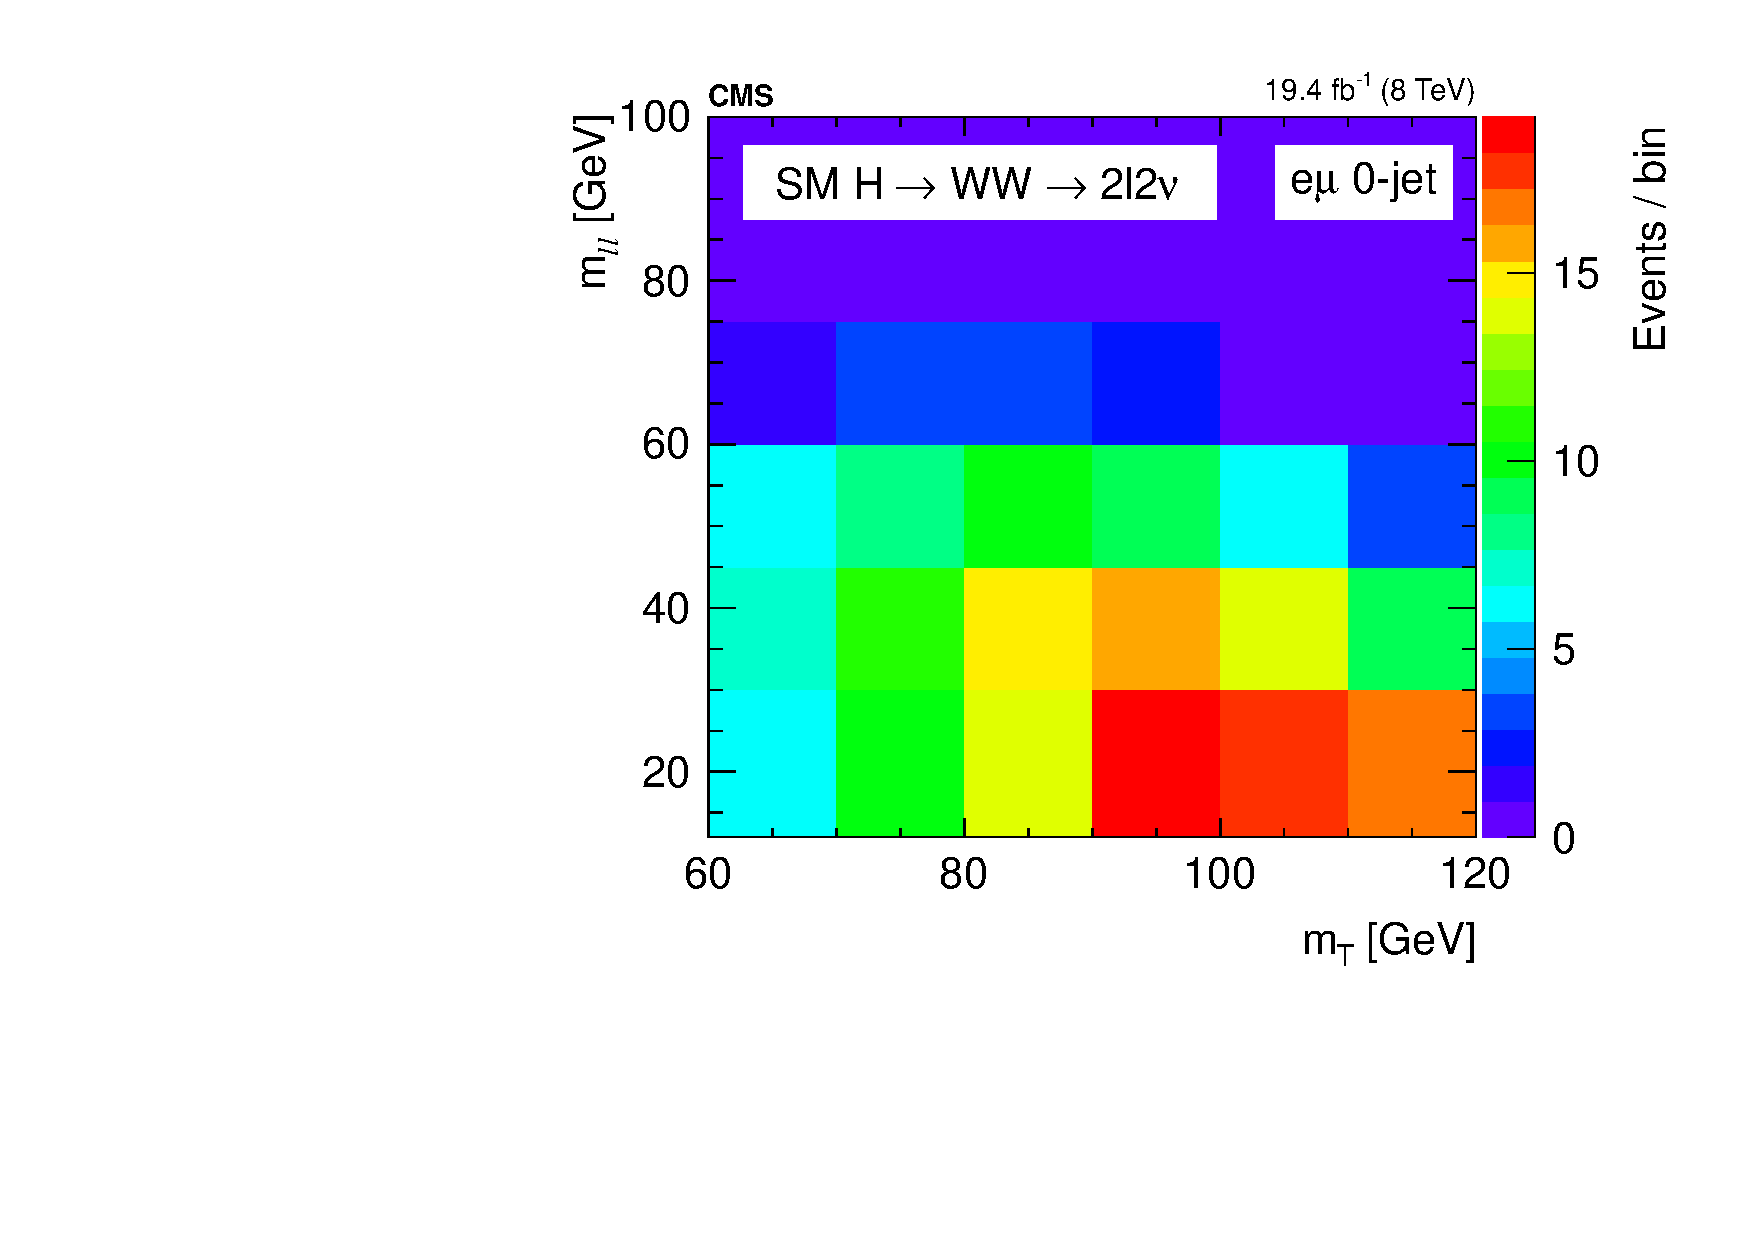
\includegraphics[width=0.45\textwidth]{images/legacyPlots/2d_prefit_0j_125_sig_paper.pdf}}
\subfigure[]{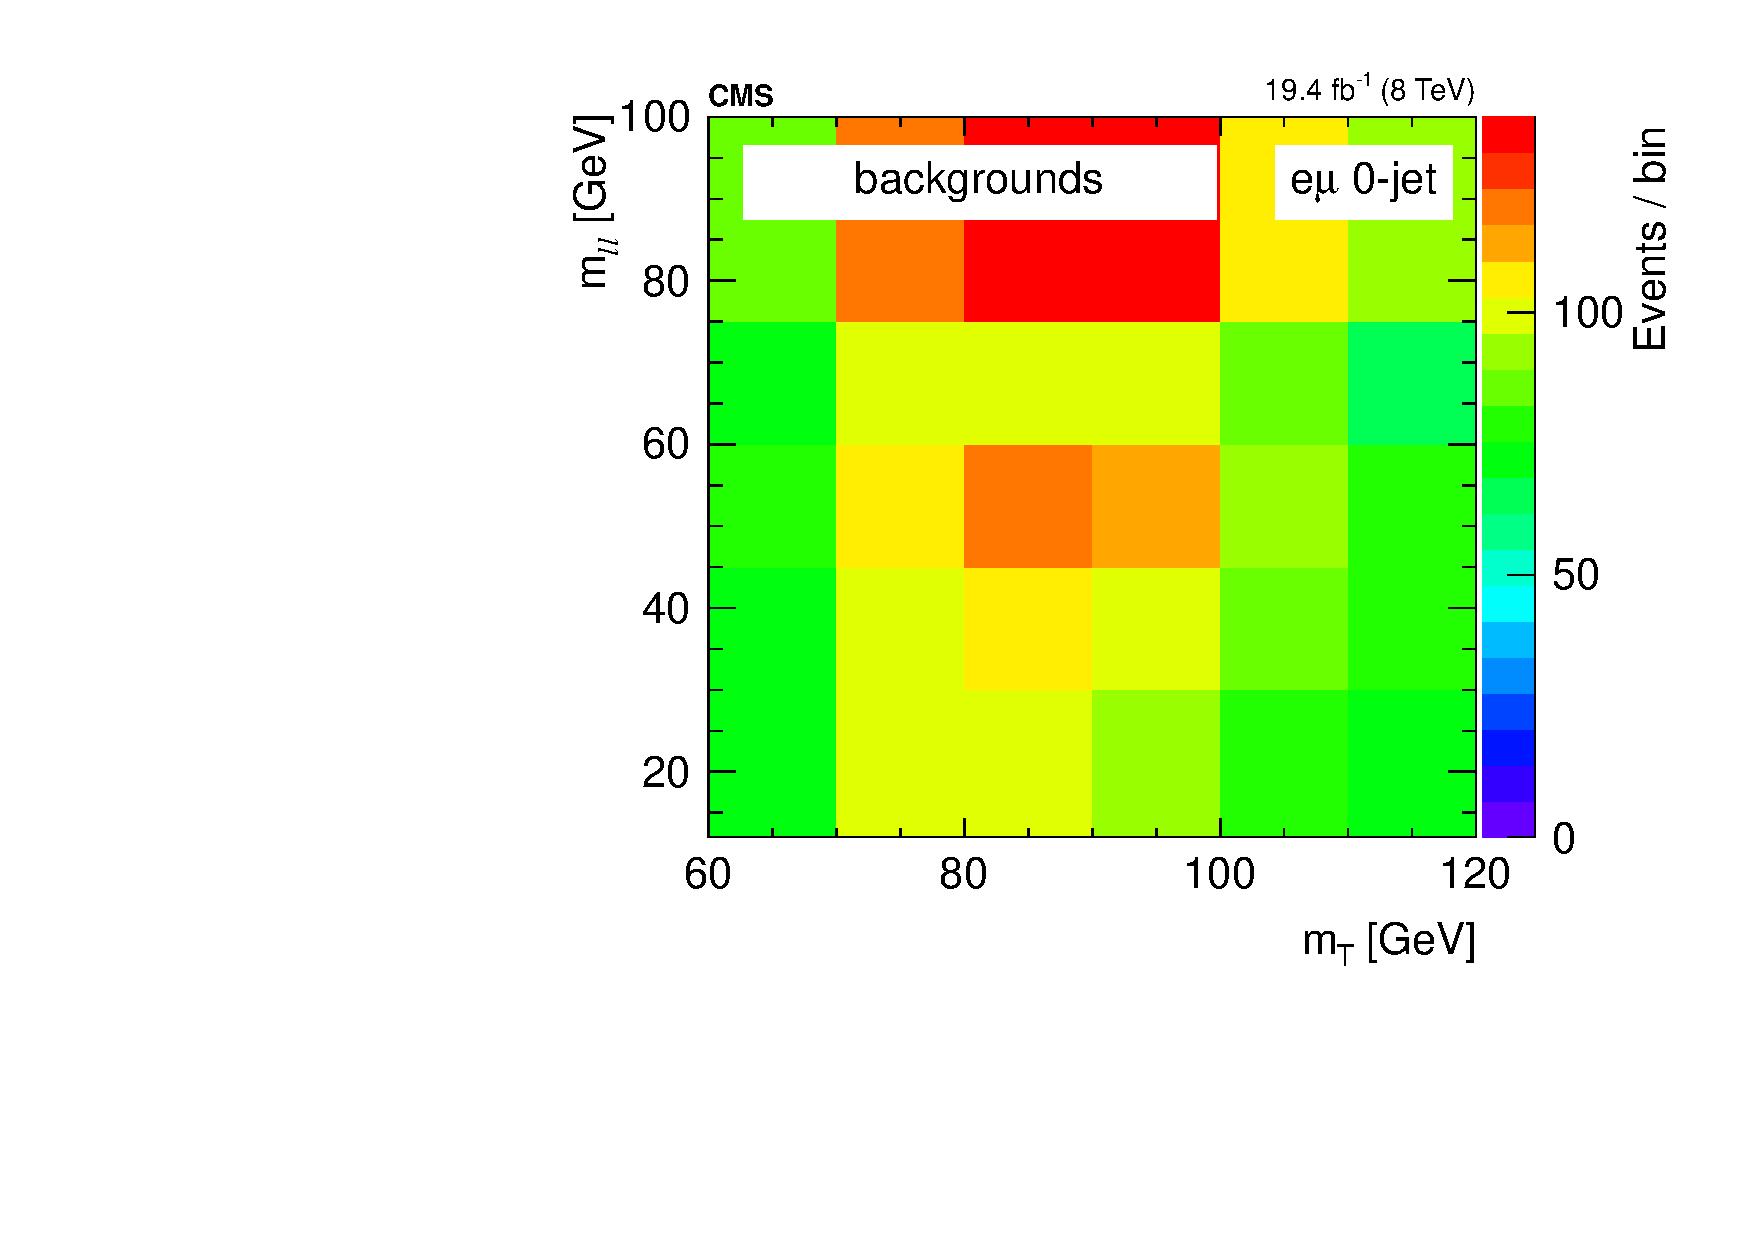
\includegraphics[width=0.45\textwidth]{images/legacyPlots/2d_prefit_0j_125_bkg_paper.pdf}}
\caption{Two-dimensional \mll--\mt distribution for signal (a) and background (b) processes in the 0 jets category.\label{fig:2Dlegacy}}
\end{figure}

Six different signal strengths are extracted from the fit, one for each \pth~bin. The relative contributions of the different Higgs production mechanisms in the signal template are taken to be the same as in the SM. The sources of systematic uncertainty are considered as nuisance parameters in the fit.

The binning of the \mll and \mt templates is chosen to be:
\begin{itemize}
\item {\mll: $[12,30,45,60,75,100,125,150,175,200]$} 
\item {\mt: $[60,70,80,90,100,110,120,140,160,180,200,220,240,280]$}
\end{itemize}

To avoid a dependence of the results on the variables used for the template fit, \mll and \mt need to be uncorrelated with respect to \pth.
This has been verified and the correlation between the discriminating variables and \pth is shown in Fig.~\ref{fig:correlation_ggH} and Fig.~\ref{fig:correlation_vbf} for ggH and VBF production modes, respectively.

\begin{figure}[htb]
\centering
\subfigure[]{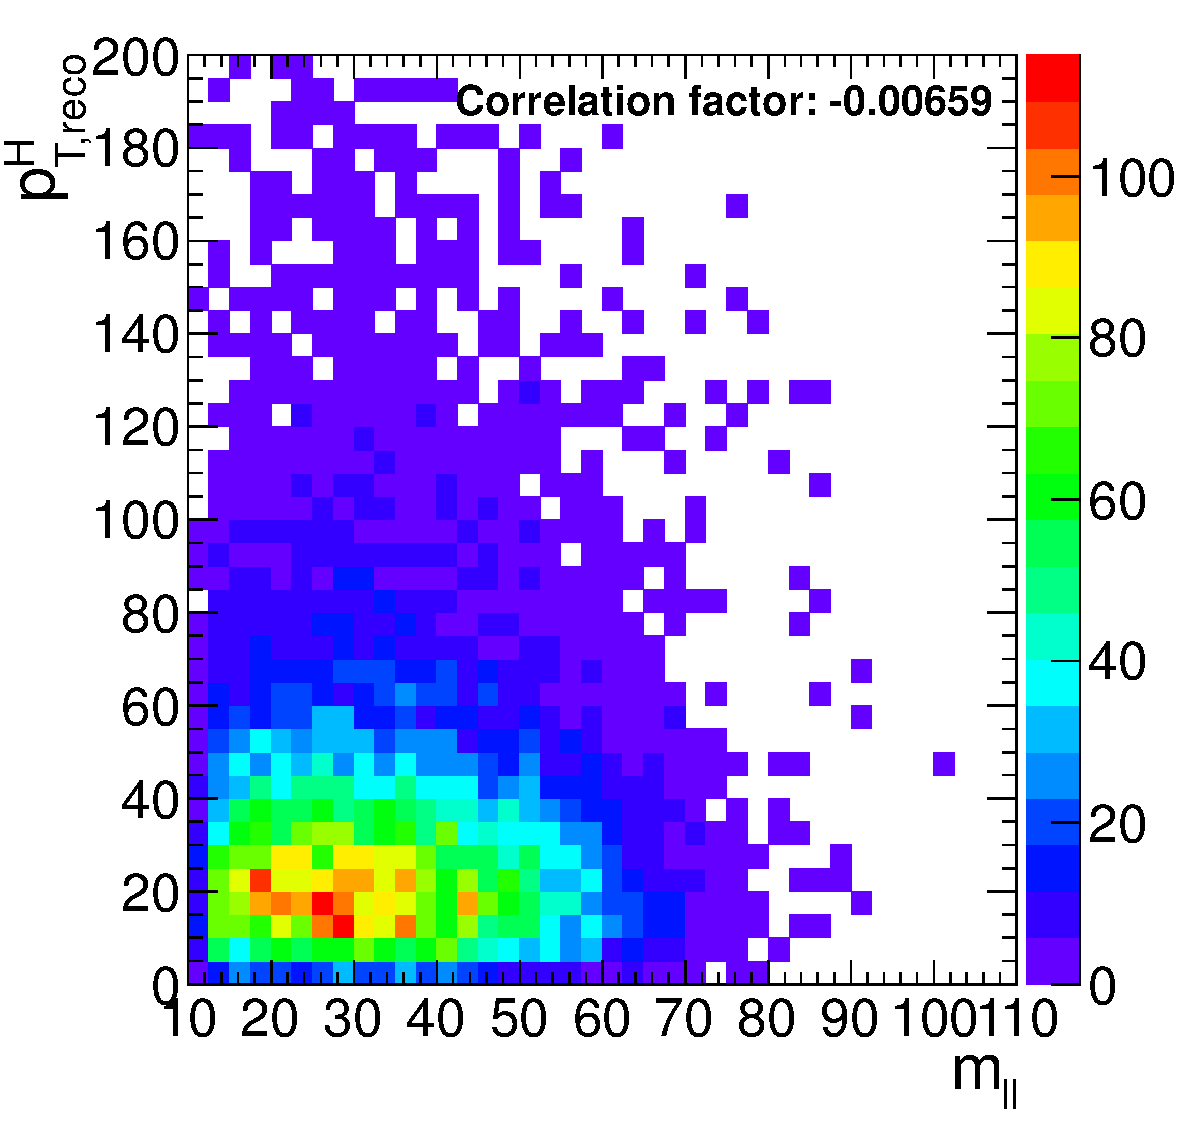
\includegraphics[width=0.45\textwidth]{images/correlationmll_ggH-v2.pdf}}
\subfigure[]{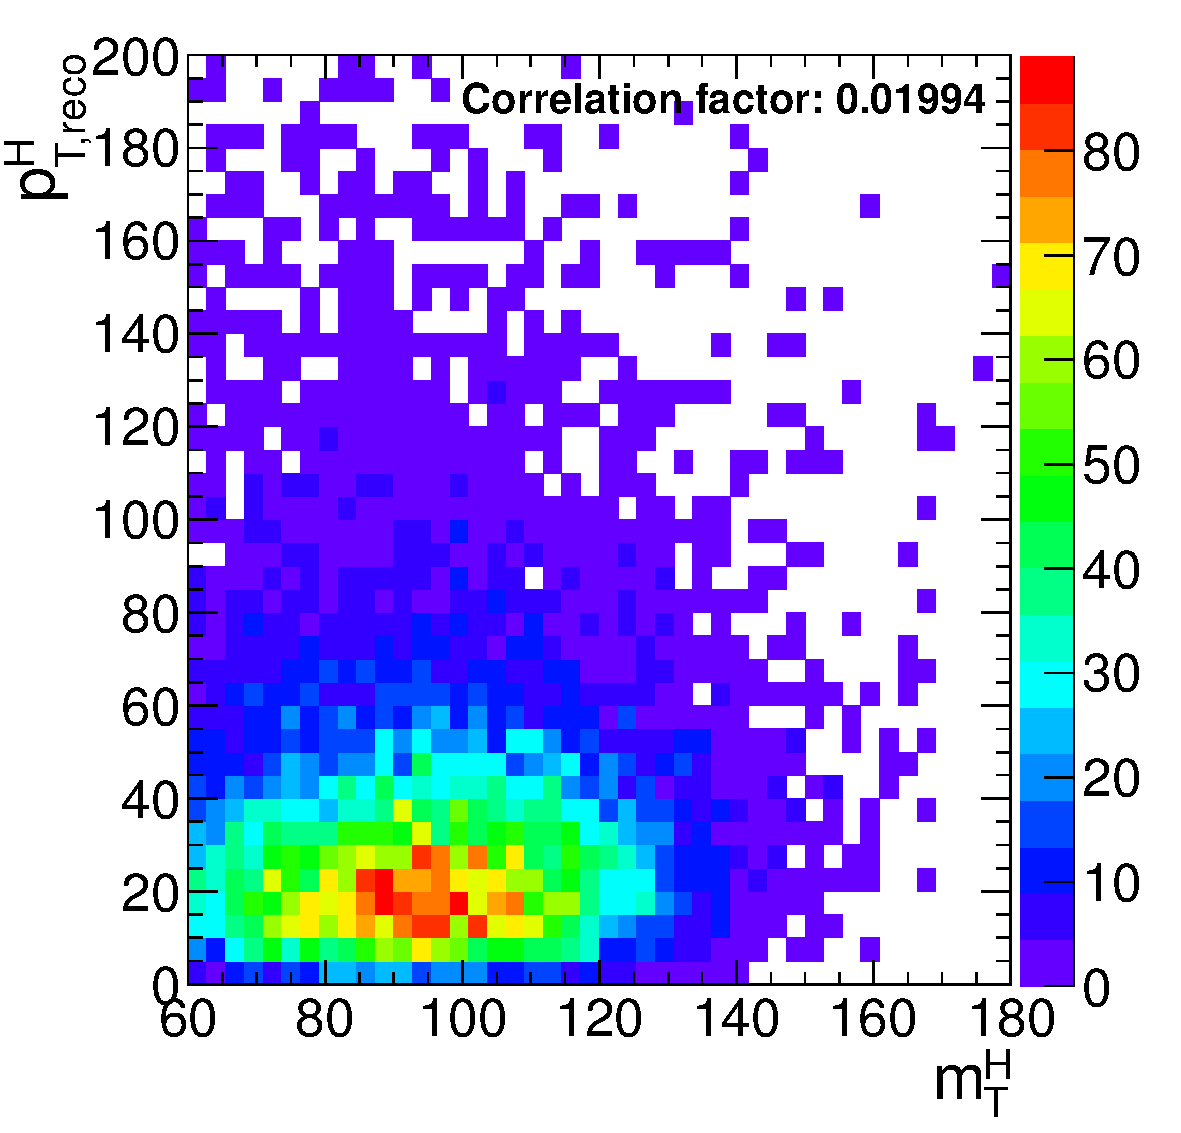
\includegraphics[width=0.45\textwidth]{images/correlationmth_ggH-v2.pdf}}
\caption{Correlation between $\pth$ and $\mll$ (a) and between \pth and \mt (b) after the full selection for the ggH production mode.\label{fig:correlation_ggH}}
\end{figure}

\begin{figure}[htb]
\centering
\subfigure[]{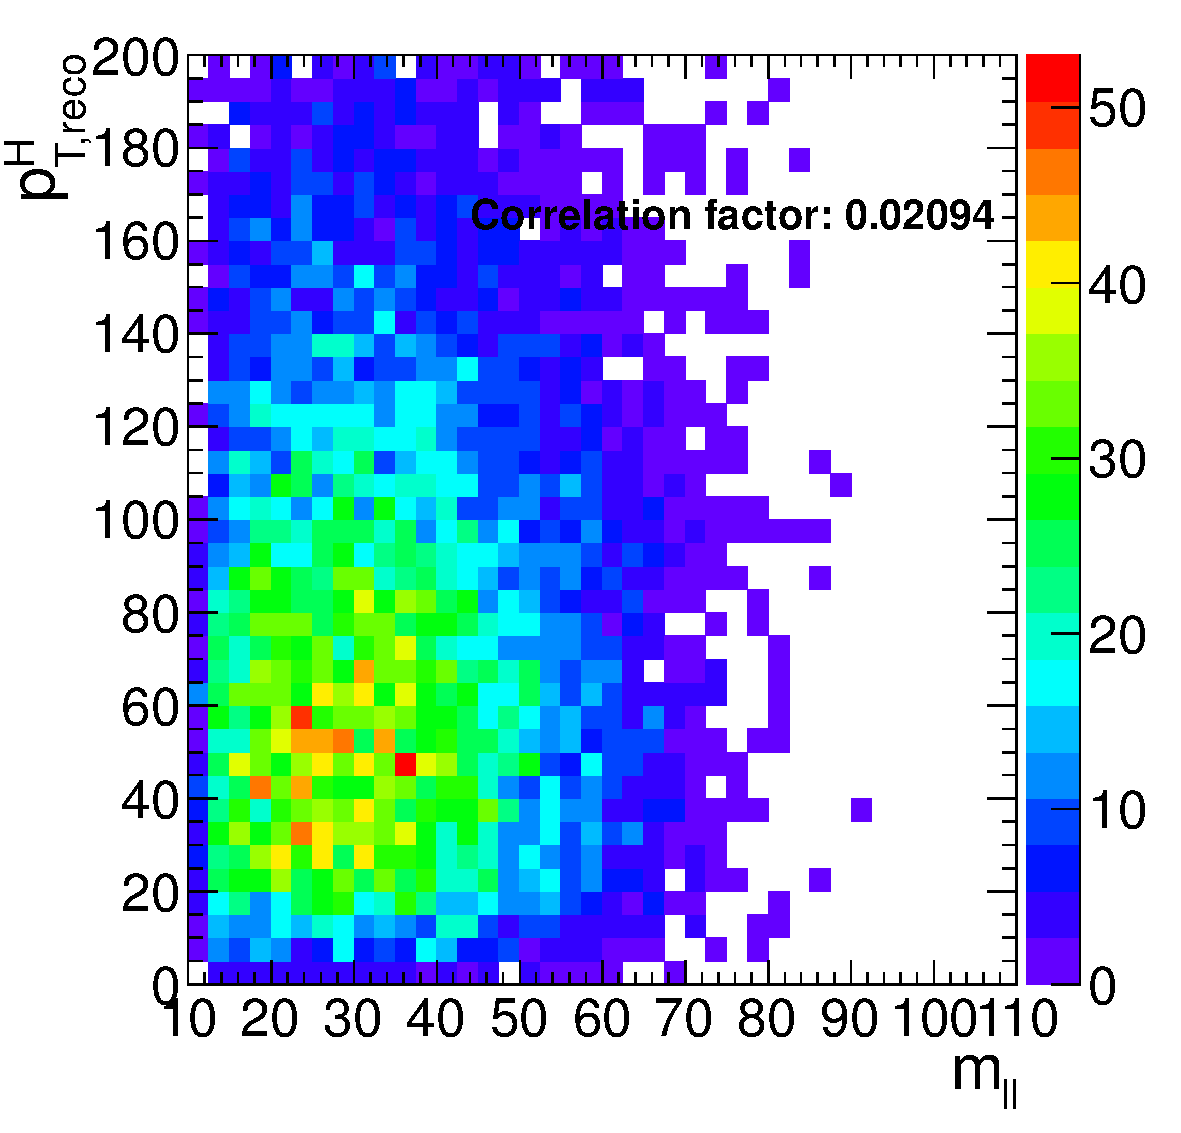
\includegraphics[width=0.45\textwidth]{images/correlationmll_vbf-v2.pdf}}
\subfigure[]{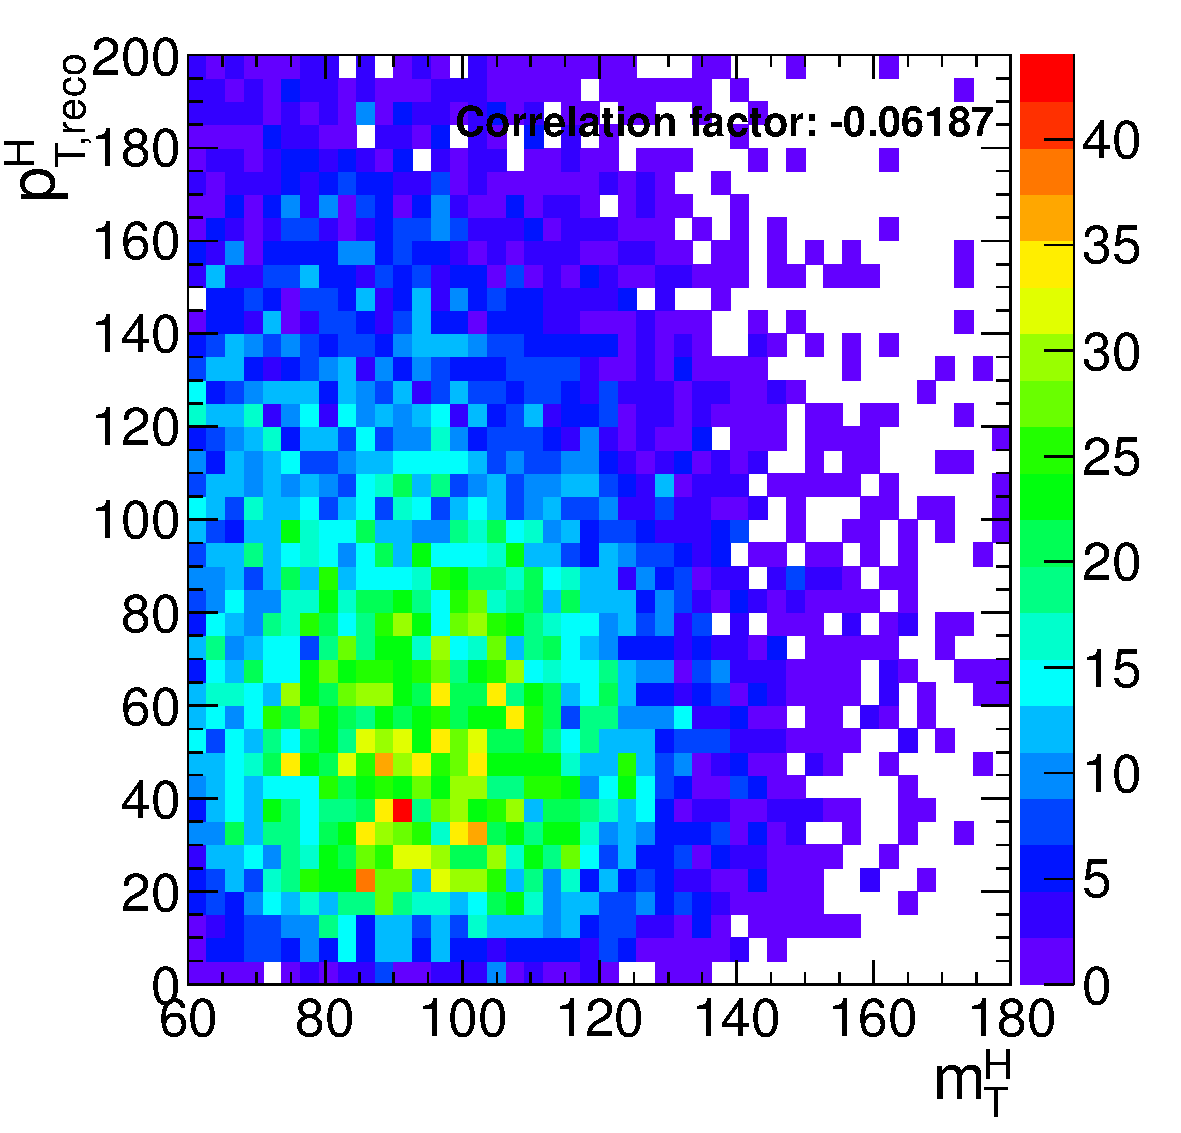
\includegraphics[width=0.45\textwidth]{images/correlationmth_vbf-v2.pdf}}
\caption{Correlation between \pth and \mll (a) and between \pth and \mt (b) after the full selection for the VBF production mode.\label{fig:correlation_vbf}}
\end{figure}

The signal strength $\mu$ in each bin, defined as the ratio between the measured cross section and the SM one, $\mu = \sigma/\sigma_\mathrm{SM}$, is allowed to float between -10 and +10, thus permitting negative values. This is mainly intended to allow future combinations with similar measurements without introducing any bias.

Because of detector resolution effects, some of the reconstructed $\hww$ signal events might originate from outside the fiducial phase space.  
These out-of-fiducial signal events cannot be precisely handled by the unfolding procedure and must be subtracted from the reconstructed spectrum. The \pth distribution of the out-of-fiducial signal events is taken from simulation, and each bin is multiplied by the corresponding measured signal strength before performing the subtraction. 

At the end, the number of events in each bin $i$ of the measured spectrum is:
\begin{equation}\label{eq:sig_yield}
N_i = \mu_i (s_i -f_i) \quad ,
\end{equation}

\noindent where $\mu_i$ is the measured signal strength, $s_i$ and $f_i$ are the total number of reconstructed signal events and the number of reconstructed out-of-fiducial signal events expected from simulation, respectively.

The fit makes use of the binned maximum likelihood approach. The likelihood function $\mathcal{L}$, restricted to the \pth bin $j$, can be written as:
\begin{equation}
\mathcal{L}(data|\mu_j,\theta) = Poisson(data|\mu_j \cdot s(\theta) + b(\theta)) \cdot p(\tilde{\theta} |\theta ) \quad ,
\end{equation}

\noindent where $Poisson(data|\mu_j \cdot s + b)$ is the product of the Poisson probabilities to observe $n_i$ events in bin $i$, i.e.:
\begin{equation}\label{eq:poisson}
\prod_i \frac{(\mu_j\cdot s_i + b_i)^{n_i}}{n_i !} e^{-\mu_j \cdot s_i - b_i} \quad.
\end{equation}

%\begin{equation}
%\mathcal{L}(\mu_j,\theta) = \prod_{i=0}^{N_\mathrm{bins}} \frac{(\mu_j s_i(\theta) + b_i(\theta))^{n_i}}{n_i!}e^{-\mu_j s_i(\theta) - b_i(\theta)} \cdot p(\tilde{\theta} |\theta ) \quad ,
%\end{equation}
Here $\mu_j$ is the signal strength in the bin $j$, i.e. the parameter of interest of the fit, which multiplies the signal yield. The index $i$ runs over the bins of the \mll-\mt two-dimensional histogram corresponding to the \pth bin $j$, $s_i$ and $b_i$ are the expected number of signal and background events respectively in bin $i$, and $n_i$ is the total number of observed events in bin $i$. The set of parameters $\theta$ represents the full suite of nuisance parameters used to incorporate the systematic uncertainties. Each nuisance parameter is constrained in the fit including the prior distribution functions $p(\tilde{\theta}|\theta)$ in the likelihood, where $\tilde{\theta}$ is the set of default values for the $\theta$ parameters~\cite{CMS-NOTE-2011-005}. For the major part of the nuisance parameters a log-normal prior distribution is used, with a standard deviation corresponding to the given systematic uncertainty. This is the optimal choice to describe uncertainties of definite positive observables, like cross sections, efficiencies, luminosity, etc. The usage of a gaussian distribution, under certain circumstances, would indeed allow the value of the observable to fluctuate below zero.
For some nuisance parameters, as the ones related to the statistical uncertainty coming from the background measurement in data control regions, a Gamma distribution is instead recommended. 
A log-uniform distribution is used for the uncertainties related to the normalization of background contributions that are left unconstrained in the fit, such as for the WW background process.
Finally, some of the experimental uncertainties related to the shape of signal and background processes are modelled by means of additional histograms as explained in Sec.~\ref{sec:syst_treatment}. The correlations of nuisance parameters across different \pth bins are taken into account. Moreover the nuisance parameters can also be correlated (or anti-correlated) between signal and different background processes. As an example, the uncertainty related to the integrated luminosity measurement is fully correlated for all the signal and background processes.

Before running the fit on the data, the same procedure has been applied to the so called \textit{Asimov data set}\footnote{In a parallel reality imagined by the science fiction writer I. Asimov, politics was run in a peculiar way: instead of mobilizing millions of people to cast their vote to deliberate on something, an algorithm was used to select an individual ``average'' person, and then this person was asked to take the decision on that matter.}, which provides a simple method to estimate the signal sensitivity before looking at the data~\cite{Cowan:2010js}.


\subsection{Signal and background yields}\label{subsec:yields}

A comparison of data and background predictions is shown in Fig.~\ref{fig:mllSignalRegion}, where the \mll{} distribution is shown for the six \pth bins. Distributions are shown in the \mt window of [60, 110]\GeV, in order to emphasize the signal contribution. The \mt distributions are shown in Fig.~\ref{fig:mTSignalRegion} and correspond to the \mll window of [12, 75]\GeV. The signal and background yields after the analysis selection are reported in Table~\ref{table:yields}.

\begin{figure}[htbp]
\centering
\subfigure{
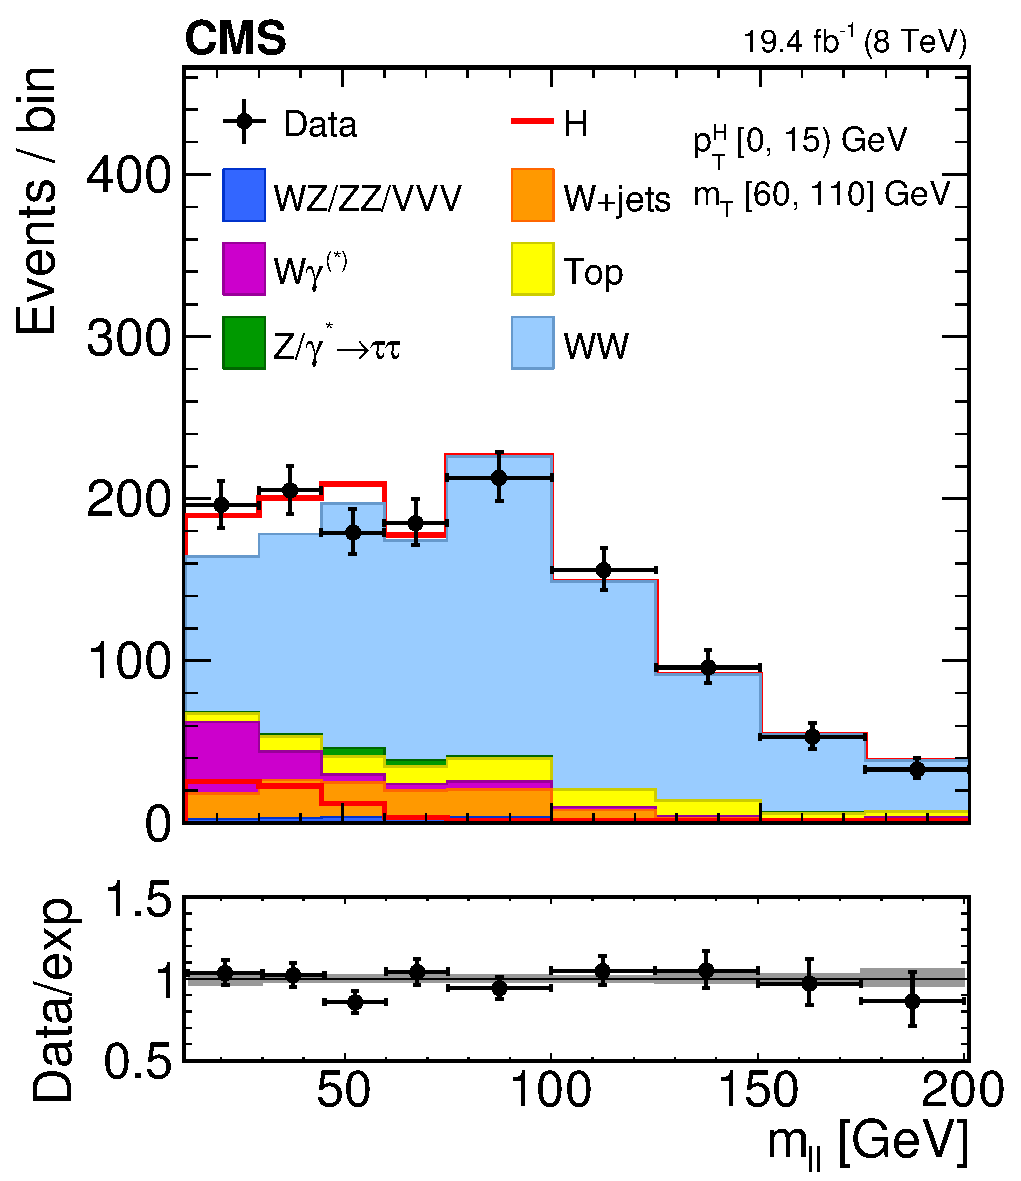
\includegraphics[width=0.3\textwidth]{images/unblinding/mllBin0.pdf}
}
\subfigure{
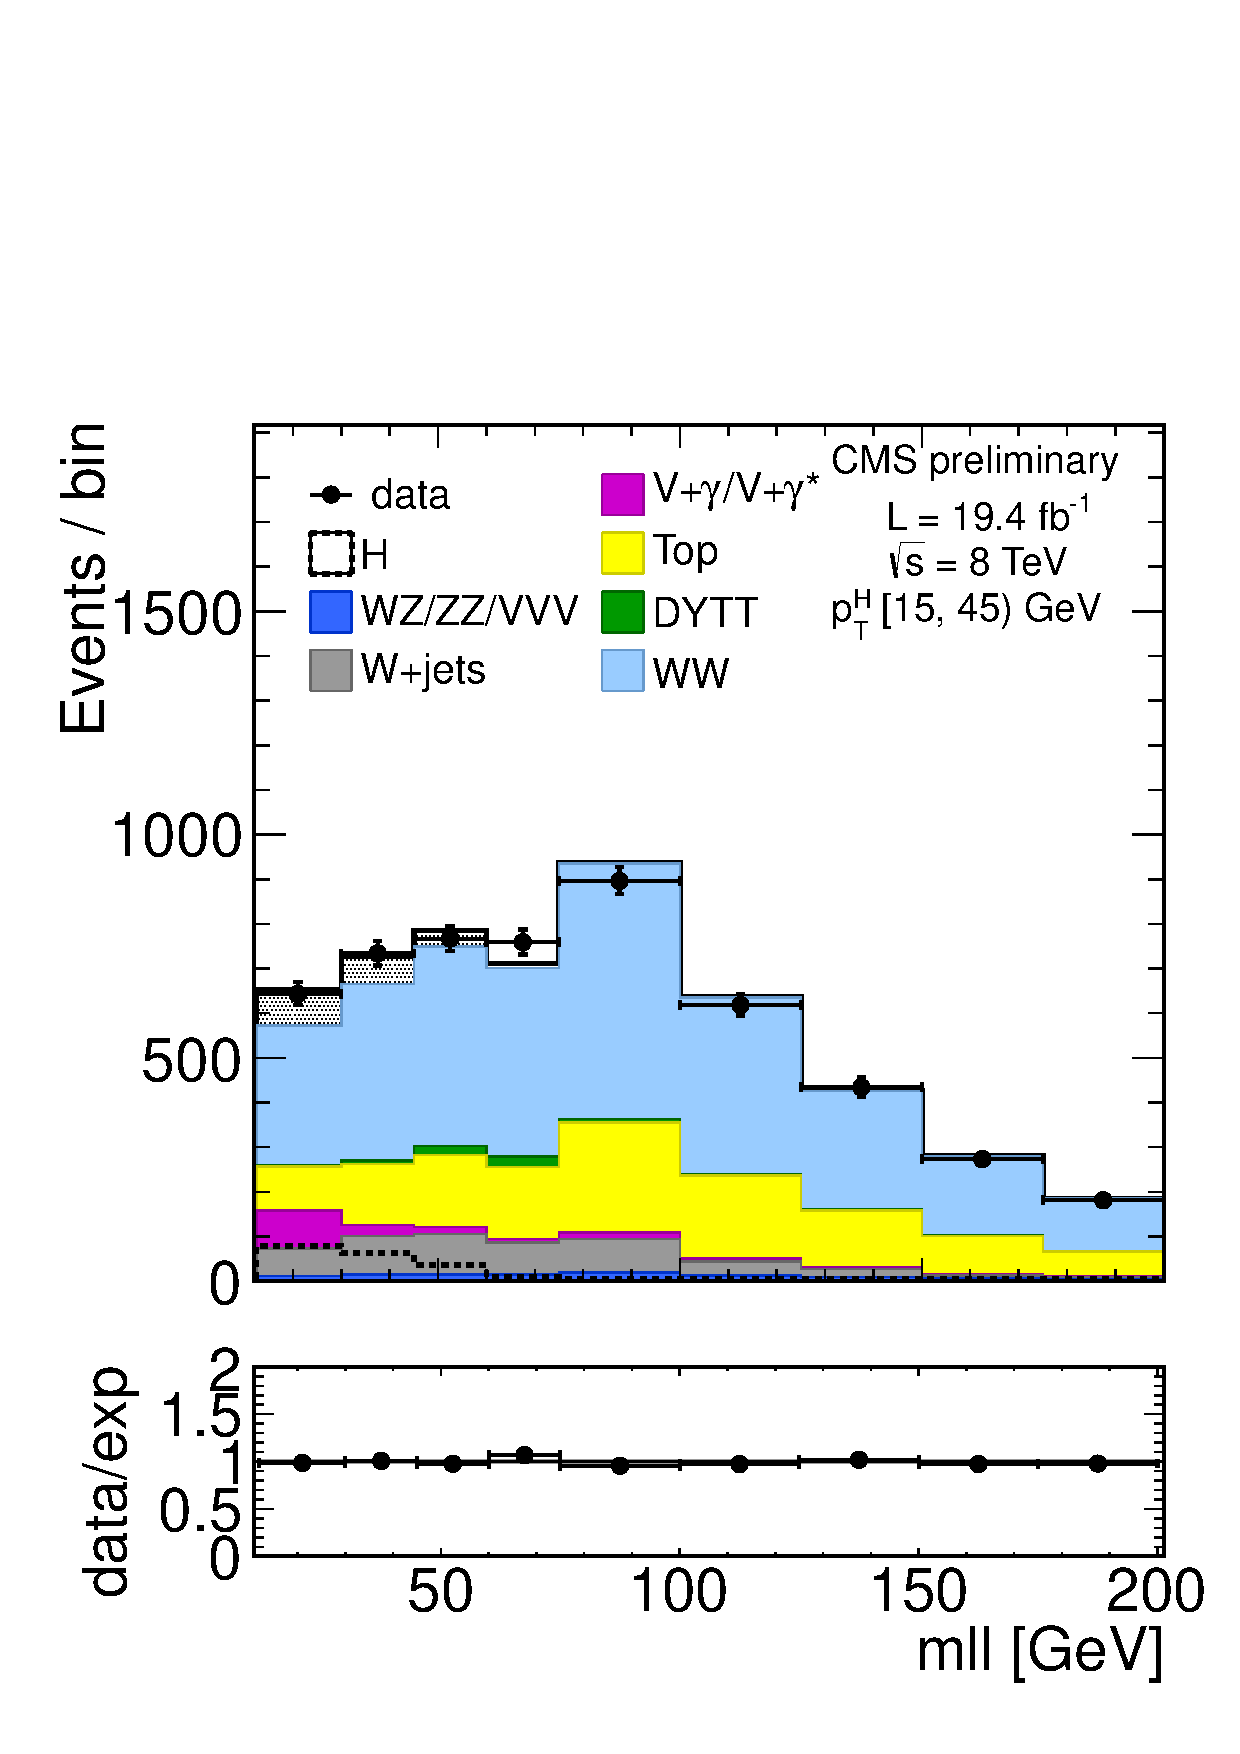
\includegraphics[width=0.3\textwidth]{images/unblinding/mllBin1.pdf}
}
\subfigure{
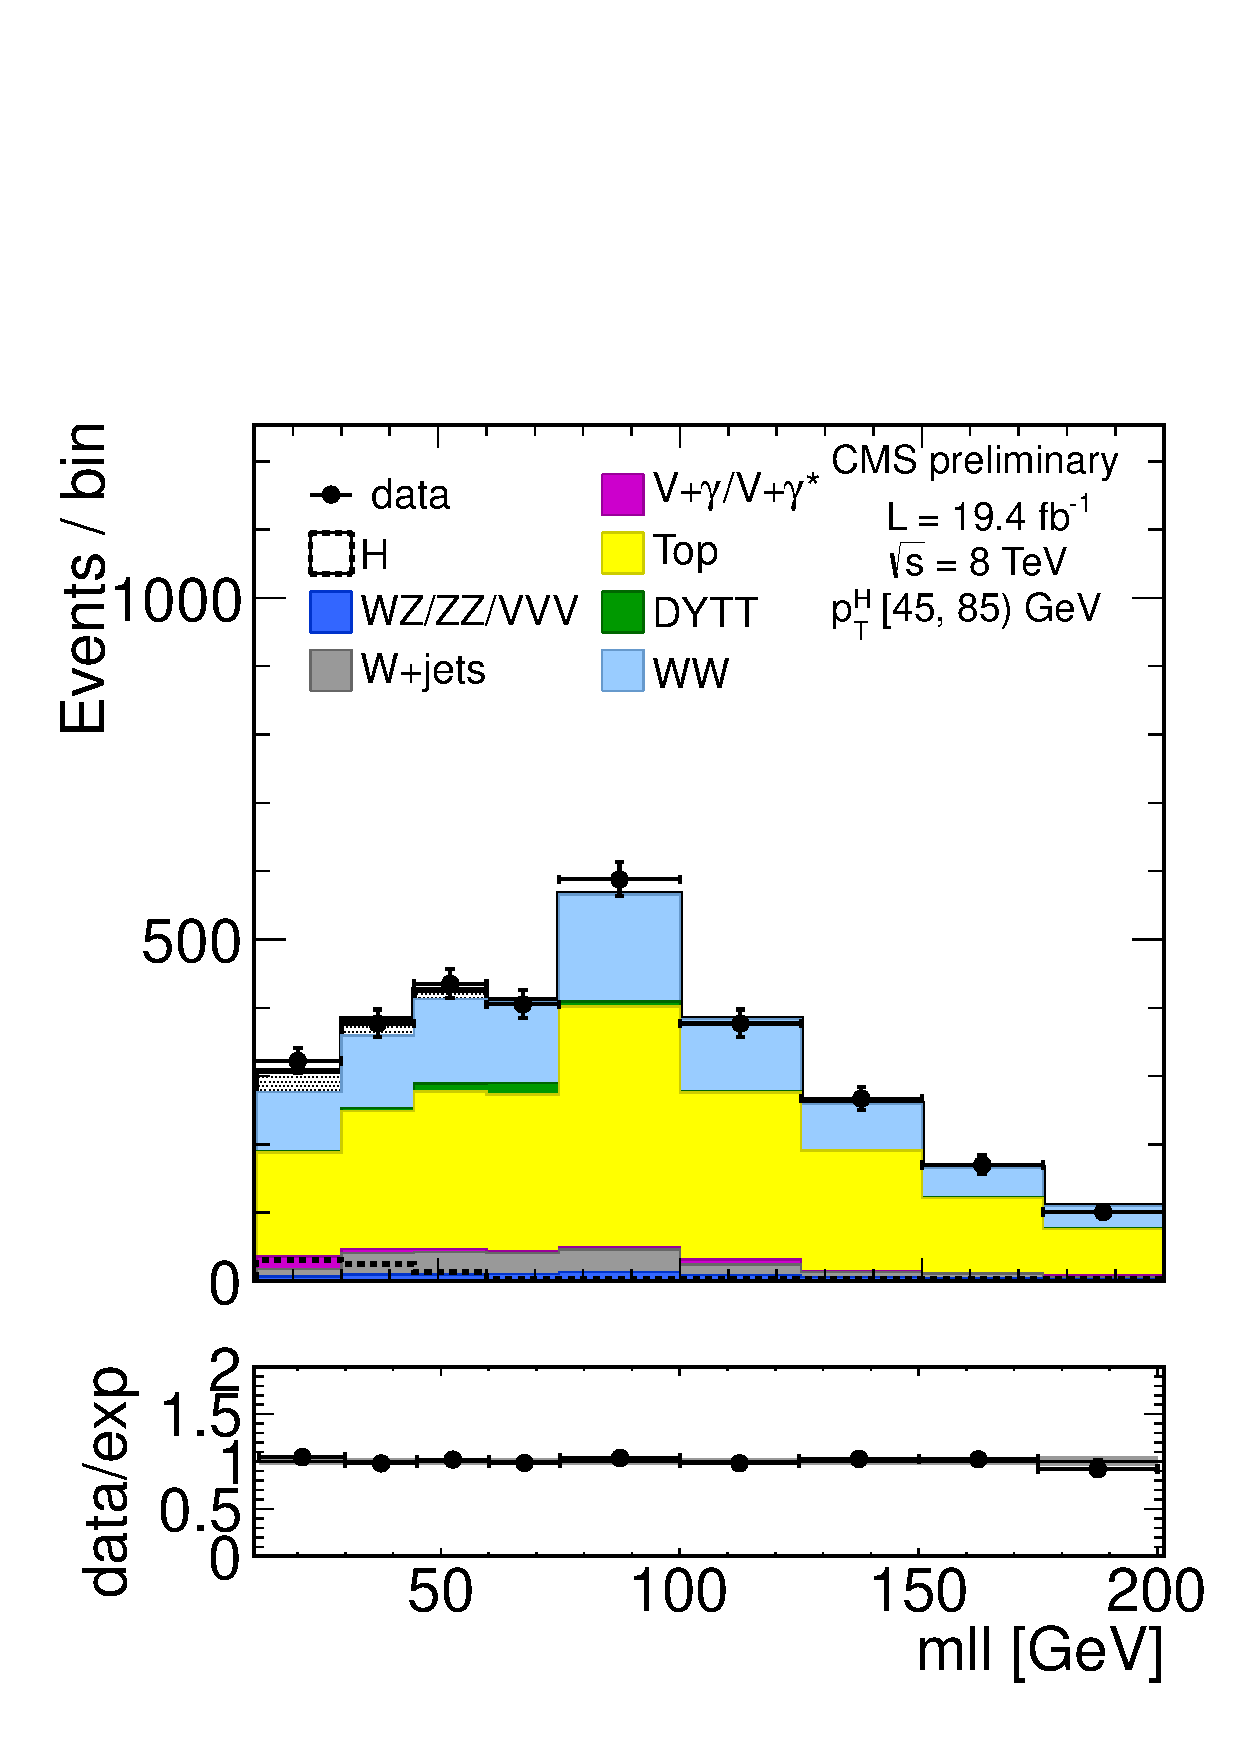
\includegraphics[width=0.3\textwidth]{images/unblinding/mllBin2.pdf}
}\\
\subfigure{
\includegraphics[width=0.3\textwidth]{images/unblinding/mllBin3.pdf}
}
\subfigure{
\includegraphics[width=0.3\textwidth]{images/unblinding/mllBin4.pdf}
}
\subfigure{
\includegraphics[width=0.3\textwidth]{images/unblinding/mllBin5.pdf}
}
\caption{Distributions of the \mll variable in each of the six \pth bins. Background normalizations correspond to the values obtained from the fit. Signal normalization is fixed to the SM expectation. The distributions are shown in an \mt window of [60,110]\GeV in order to emphasize the Higgs boson (H) signal. The signal contribution is shown both stacked on top of the background and superimposed on it. Ratios of the expected and observed event yields in individual bins are shown in the panels below the plots. The uncertainty band shown in the ratio plot corresponds to the envelope of systematic uncertainties after performing the fit to the data.}\label{fig:mllSignalRegion}
\end{figure}

\begin{figure}[htbp]
\centering
\subfigure{
\includegraphics[width=0.3\textwidth]{images/unblinding/mTBin0.pdf}
}
\subfigure{
\includegraphics[width=0.3\textwidth]{images/unblinding/mTBin1.pdf}
}
\subfigure{
\includegraphics[width=0.3\textwidth]{images/unblinding/mTBin2.pdf}
}\\
\subfigure{
\includegraphics[width=0.3\textwidth]{images/unblinding/mTBin3.pdf}
}
\subfigure{
\includegraphics[width=0.3\textwidth]{images/unblinding/mTBin4.pdf}
}
\subfigure{
\includegraphics[width=0.3\textwidth]{images/unblinding/mTBin5.pdf}
}
\caption{Distributions of the \mt variable in each of the six \pth{} bins. Background normalizations correspond to the values obtained from the fit. Signal normalization is fixed to the SM expectation. The distributions are shown in an \mll window of [12,75]\GeV in order to emphasize the Higgs boson (H) signal. The signal contribution is shown both stacked on top of the background and superimposed on it. Ratios of the expected and observed event yields in individual bins are shown in the panels below the plots. The uncertainty band shown in the ratio plot corresponds to the envelope of systematic uncertainties after performing the fit to the data.}\label{fig:mTSignalRegion}
\end{figure}

\begin{table}[htb]
\footnotesize{
\begin{center}{
  \caption{Signal prediction, post-fit background estimates and observed number of events in data are shown in each \pth{} bin after applying the analysis selection requirements. The total uncertainty in the number of events is reported. For signal processes, the yield related to ggH are shown, separated with respect to the contribution of the other production mechanisms (XH=VBF+VH). The WW process includes both quark and gluon induced contributions, while the Top process takes into account both \ttbar and tW. }\label{table:yields}
\begin{tabularx}{\textwidth}{ l >{\centering}X >{\centering}X >{\centering}X >{\centering}X >{\centering}X >{\centering}X }

\toprule

\multirow{2}{*}{Process} & \multicolumn{6}{c}{\pth [\GeV]} \tabularnewline
 &	0--15	&	15--45	&	45--85	&	85--125	&	125--165	&	165--$\infty$ \tabularnewline

\midrule

ggH	&	$73\pm3$	&	$175\pm5$	&                $59\pm3$	&                $15\pm2$	&                $5.1\pm1.5$	&                $4.9\pm1.4$	\tabularnewline
XH=VBF+VH	&	$4\pm2$ 	&	$15\pm4$ 	&		 $16\pm4$	&	         $8\pm2$ 	&		 $3.8\pm1.1$ 	&		 $3.0\pm0.8$    \tabularnewline
Out-of-fiducial & $9.2\pm0.5$   &       $19.9\pm0.7$    &      $11.4\pm0.6$    &    $4.4\pm0.3$   &     $1.6\pm0.2$   &   $2.4\pm0.2$ \tabularnewline
Data 	&	2182	 	&         5305	 	&	         3042	 	& 	          1263	 	&	         431	 	& 	          343	 	\tabularnewline
Total background &  	 $2124\pm128$	 &     $5170\pm321$	 &       $2947\pm293$	 &            $1266\pm175$	 &         $420\pm80$	 &              $336\pm74$	 \tabularnewline

WW 	& 		$1616\pm107$	 &	 $3172\pm249$	 &	     $865\pm217$	 &	     $421\pm120$	 &	     $125\pm60$	 &		     $161\pm54$	 \tabularnewline
Top 	&	$184\pm38$	&	                $1199\pm165$	&	                $1741\pm192$	&	                $735\pm125$	&	                $243\pm51$	& 	        $139\pm49$	\tabularnewline
W+jets 	& $134\pm5$ 	&	         $455\pm10$ 	&	         $174\pm6$ 	&	         $48\pm4$ 	&	         $14\pm3$ 	&	         $9\pm3$ 	\tabularnewline
WZ+ZZ+VVV & $34\pm4$ 	 &	$107\pm10$ 	&                $71\pm7$ 	&	         $29\pm5$ 	&                $14\pm3$ 	&     $13\pm4$ 	\tabularnewline
\dytt 	&	$23\pm3$ 	&         $67\pm5$ 	&         $47\pm4$ 	&         $22\pm3$ 	&         $12\pm2$ 	&         $10\pm2$ 	\tabularnewline
W$\gamma^{(*)}$	& $132\pm49$     &             $170\pm58$    &              $48\pm30$ &                  $12\pm9$ &                  $3\pm3$ &                 $5\pm10$ \tabularnewline

\bottomrule

  \end{tabularx}
  }
   
  \end{center}
  }
\end{table}

The signal strengths obtained performing the fit are shown in Table~\ref{tab:signal_strengths}.
In order to assess the robustness of the fit, several toy MC samples have been generated with a mean value for each bin corresponding to the sum of the expected background plus signal events and a statistical accuracy comparable to the one expected in data. Each toy sample is fitted with the same procedure described before. The distribution of the signal strengths extracted in each bin using the toy MC samples are found to be consistent with 1, implying that no bias is introduced by the fit procedure. 
%Moreover, the pull distribution of each signal strength has also been checked, showing an average and RMS value consistent with 0 and 1, respectively.

\begin{table}[htb]
\caption{Signal strengths measured in data for each \pth bin with 68$\%$ CL uncertainties.}\label{tab:signal_strengths}
\begin{center}
\begin{tabular}{ c  c  c  } \toprule
 \pth [GeV] & $\mu$  & Uncertainty (68$\%$ CL) \\ \midrule
 0--15   &  +0.753  & -0.424/+0.437  \\
 15--45   &  +0.716  & -0.300/+0.308  \\
 45--85   &  +1.309  & -0.445/+0.465  \\
 85--125   &  +0.165  & -0.890/+0.898  \\
 125--165   &  +1.715  & -1.103/+1.217  \\
 165--$\infty$   &  +0.796  & -0.913/+1.059  \\
 \bottomrule
\end{tabular}
\end{center}
\end{table}

%\begin{figure}[htb]
%\centering
%\subfigure[]{\includegraphics[width=0.45\textwidth]{images/mu_toys.pdf}}
%\subfigure[]{\includegraphics[width=0.45\textwidth]{images/pull_toys.pdf}}
%\caption{Signal strength distribution as extracted from the fit of toy MC samples (a). Distribution of the pull of the signal strength parameters (b).\label{fig:pull_fit}}
%\end{figure}


%The signal yield after the fit with data is found to be of $318 \pm 12$ events, to be compared with the expected value of $382 \pm 7$ events.
The reconstructed spectrum is obtained starting from the signal yield $N_i$ in each \pth bin $i$ and dividing it by the bin width $w_i$ and integrated luminosity $\mathcal{L}$, i.e.:
\begin{equation}
\frac{d\sigma_i}{d p_\mathrm{T,reco}^\mathrm{H}} = \frac{N_i}{w_i \mathcal{L}} \quad.
\end{equation}

The spectrum shown in Fig.~\ref{fig:pre_unfolding} is obtained after having performed the fit and after the subtraction of the out-of-fiducial signal events, but before undergoing the unfolding procedure. The theoretical distribution after the detector simulation and event reconstruction is also shown for comparison. Also, the expected distribution of the subdominant VBF and VH production mechanisms is displayed.

\begin{figure}[htb]
\centering
\includegraphics[width=0.7\textwidth]{images/unblinding/pth_reco_paper.pdf}
\caption{Differential Higgs boson production cross section as a function of the reconstructed \pth{}, before applying the unfolding procedure. Data values after the background subtraction are shown together with the statistical and the systematic uncertainties, determined propagating the sources of uncertainty through the fit procedure. The line and dashed area represent the SM theoretical estimates in which the acceptance of the dominant ggH contribution is modelled by \textsc{Powheg V1}. The subdominant component of the signal is denoted as XH=VBF+VH, and is shown with the cross filled area separately.}\label{fig:pre_unfolding}
\end{figure}

In order to measure the inclusive cross section times branching fraction in the fiducial phase space, the reconstructed differential spectrum of Fig.~\ref{fig:pre_unfolding} is integrated over \pth. The contribution of the uncertainty in each bin is propagated to the inclusive measurement taking into account the correlations of the signal strengths, i.e. using the covariance matrix. For the extrapolation of this result to the fiducial phase space the unfolding procedure is not needed and the inclusive measurement has only to be corrected for the fiducial phase space selection efficiency $\epsilon_{\rm{fid}} = 36.2\%$. The inclusive fiducial cross section times branching fraction $\sigma_{\mathrm{fid}}$ is computed to be:
\begin{equation}
\sigma_{\mathrm{fid}} = 39\pm 8~(\mathrm{stat}) \pm 9~(\mathrm{syst})~\mathrm{fb} \quad ,
\end{equation} 

\noindent in agreement within uncertainties with the theoretical estimate of $48 \pm 8 ~\mathrm{fb}$, computed integrating the simulated spectrum obtained with the \textsc{Powheg V2} generator for the ggH process, scaled to the NNLO+NNLL cross section, and including the XH contribution.


%\clearpage
\section{Unfolding}
%%%%%%%%%%%%%%%%%%%%%%%%%%%%%%%%%%%%%%%%%%%%%%%%%%%%%%%%%%%%%%%%%%%%%%
\label{sec:Unfolding}

To facilitate comparisons with theoretical predictions or other experimental results, the signal
extracted performing the fit has to be corrected for detector resolution and
efficiency effects and for the efficiency of the selection defined in the
analysis.
An unfolding procedure is used relying on the \textsc{RooUnfold} package
\cite{Adye:2011gm}, which provides the tools to run various unfolding
algorithms.

The basic principle behind the unfolding procedure in this analysis is to use MC signal samples to obtain both the ``true'' distribution of the variable of interest before particle interactions with the detector, and the distribution in reconstructed events after the full \textsc{Geant4} simulation of the CMS detector and event reconstruction.
These two distributions are used to calculate the detector response matrix $M$, defined by the following equation:
\begin{equation}\label{eq:resp_matrix}
R_{i}^{\rm {MC}} = \sum_{j=1}^{n} M_{ij}T_{j}^{\rm {MC}} \quad ,
\end{equation}

\noindent where $T^{\rm{MC}}$ and $R^{\rm{MC}}$ are two $n$-dimensional vectors
representing the distribution before and after event processing through CMS
simulation and reconstruction. The dimension $n$ of the two vectors corresponds 
to the number of bins in the distributions, equal to six in this analysis.
The response matrix $M$ includes all the effects related to the detector and analysis selection that affect the $R^{\rm{MC}}$ distribution.
The goal of the unfolding procedure is to obtain the $T^{\rm{truth}}$ distribution starting from the measured
$R^{\rm{observed}}$ distribution by inverting the matrix $M$.
%To avoid the large variance and strong negative correlation between the neighbouring bins~\cite{Cowan:2002in}, 

Given the finite data statistical accuracy, a simple inversion could lead to large fluctuations in the bins of the unfolded spectrum. In particular, if the off-diagonal elements of the response matrix are sizeable, the unfolded distribution has large variance and strong negative correlations between the neighbouring bins~\cite{Cowan:2002in}. Several unfolding methods with regularization are available in literature, such as a method based on the Bayes' theorem, which overcomes the unfolding instability using an iterative procedure~\cite{DAgostini:1994zf}.

The unfolding procedure in this analysis relies on the Singular Value Decomposition (SVD)~\cite{Hocker:1995kb} method based on the Tikhonov regularization function. Such method introduces a regularization function that controls the smoothness of the distribution and depends generally on one regularization parameter, which can be tuned to achieve the desired degree of smoothness.
The choice of the regularization parameter is particularly critical, and it should represent an optimal trade-off between taming the fluctuations in the unfolded result, and biasing the unfolded distribution.
The main feature of this method is the use of the singular value decomposition of the response matrix, including an additional term to suppress the oscillatory component of the solution, i.e. the regularization term, which represents some \textit{a priori} knowledge of the final solution.
The regularization parameter $k_\mathrm{reg}$ is chosen to obtain results that are robust against numerical instabilities and statistical fluctuations, following the prescription described in Ref.~\cite{Hocker:1995kb}. This prescription consists in the diagonalization of the response matrix using the SVD approach and in the subsequent calculation of the vector $\vec{d}$, whose values $d_i$ represent the measured distribution expressed in a specific base defined by the SVD decomposition. Plotting $\log|d_i|$ as a function of $i$, where $i$ is related to the amount of regularization, one should obtain a curve that flattens out at some value of $i$. The regularization parameter corresponding to that value represents the optimal $k_\mathrm{reg}$ choice. The parameter obtained using this prescription with toy MC samples is $k_\mathrm{reg} = 3$.

The detector response matrix is built as a two-dimensional histogram, with the generator level \pth on the $y$ axis and the same variable after the reconstruction on the $x$ axis, using the same binning for both distributions.

The resulting matrix, including all signal sources and normalized by row, is shown in Fig.~\ref{fig:matrix}(a).
The diagonal bins correspond to the stability $S$, defined as the ratio of the number of events generated and reconstructed in a given bin, and the number of events generated in that bin. The same matrix, normalized by column, is shown in Fig.~\ref{fig:matrix}(b). In this case the diagonal bins correspond to the purity $P$, defined in Eq.\eqref{eq:purity}. The $S$ and $P$ parameters provide an estimate of the \pth resolution and migration effects, whose main source is the limited resolution in the measurement of \MET.

\begin{figure}[htb]
\centering
\subfigure[Response matrix normalized by row]{
\includegraphics[width=0.45\textwidth]{images/matrix_byrow_paper.pdf}
}
\subfigure[Response matrix normalized by column]{
\includegraphics[width=0.45\textwidth]{images/matrix_bycol_paper.pdf}
}
\caption{Response matrix normalized by row (a) and  by column (b) including all signal processes. The matrices are normalized either by row or by column in order to show the purity or stability in diagonal bins.}\label{fig:matrix}
\end{figure}

Several tests are performed in order to validate the unfolding procedure. To estimate the uncertainty in the unfolding procedure due to the
particular model adopted for building the response matrix, two independent ggH samples are used, corresponding to two different generators: \textsc{Powheg V1} and \textsc{JHUGen} generators, both interfaced with \textsc{Pythia 6.4}.
The \textsc{JHUGen} generator sample is used to build the response matrix while the
\textsc{Powheg V1} sample is used to build the \pth spectra at generator and reconstructed level. The reconstructed spectrum obtained using \textsc{Powheg V1} is then unfolded using the response matrix built with \textsc{JHUGen}, and the unfolded spectrum is compared to the \textsc{Powheg V1} spectrum at generator level. The result of this test shows good agreement between the two distributions.

In order to further prove the choice of the regularization parameter, a large number of simulated pseudo-experiments has been generated to verify that the coverage of the unfolded uncertainties obtained with this procedure is as expected.
From each pseudo-experiment the reconstructed \pth spectrum is obtained and then unfolded using the procedure described above, including only the statistical uncertainties. The response matrix used for this test is different from the nominal matrix, and is obtained by changing the relative ggH and VBF fractions in order to obtain a modified spectrum with respect to the SM one.
The coverage is calculated for each \pth bin, counting the number of pseudo-experiments for which the statistical uncertainty covers the true value. The results are shown in Table~\ref{tab:coverage} for different values of the regularization parameter: starting from $k_\mathrm{reg}=2$ (stronger regularization) up to $k_\mathrm{reg}=5$ (weaker regularization). The criterion for choosing the best $k_\mathrm{reg}$ value is to increase the regularization as much as possible without introducing a bias, i.e. until a 68\% coverage is fulfilled. This criterion leads to the same result as the prescription described before, strengthening the choice of $k_\mathrm{reg}=3$.

\begin{table}[htb]
\centering
\caption{Coverage interval for each bin and for different values of the regularization parameter, obtained using pseudo-experiments.}\label{tab:coverage}
\begin{tabular}{lcccc}
\toprule
\multirow{2}{*}{\pth bin [GeV]} & \multicolumn{4}{c}{Coverage} \\
 & $k_\mathrm{reg}=2$ & $k_\mathrm{reg}=3$ & $k_\mathrm{reg}=4$ & $k_\mathrm{reg}=5$\\
\midrule
0--15 	      & $0.654\pm0.016$ & $0.704\pm0.015$ & $0.727\pm0.015$ & $0.755\pm0.014$ \\
15--45 	      & $0.701\pm0.015$ & $0.665\pm0.016$ & $0.683\pm0.015$ & $0.733\pm0.015$ \\
45-85 	      & $0.717\pm0.015$ & $0.706\pm0.015$ & $0.709\pm0.015$ & $0.716\pm0.015$ \\
85--125       & $0.634\pm0.016$ & $0.681\pm0.015$ & $0.714\pm0.015$ & $0.739\pm0.015$ \\
125--165      & $0.599\pm0.016$ & $0.650\pm0.016$ & $0.700\pm0.015$ & $0.751\pm0.014$ \\
165--$\infty$ & $0.632\pm0.016$ & $0.674\pm0.015$ & $0.701\pm0.015$ & $0.722\pm0.015$ \\
\bottomrule
\end{tabular}
\end{table}



\subsection{Treatment of systematic uncertainties in the unfolding}\label{sec:uncunf}

An important aspect of this analysis is the treatment of systematic
uncertainties and their propagation through the unfolding procedure.
The sources of uncertainty are divided into three categories, depending
on whether the uncertainty affects only the signal yield (type A), both the signal
yield and the response matrix (type B), or only the response matrix (type C).
These three classes propagate differently through the unfolding procedure.

Type A uncertainties are extracted directly from the fit in the form of a covariance
matrix, which is passed to the unfolding tool as the covariance
matrix of the measured distribution. The nuisance parameters belonging to this category
are mainly the background shape and normalization uncertainties.
To extract the effect of type A uncertainties a dedicated fit is performed fixing to constant all the nuisance parameters in the model but type A ones.
The correlation matrix among the six signal strengths corresponding to the six \pth bins, including all type A uncertainties, is shown in Fig.~\ref{fig:typeA_corr}.
The correlation cor($i$,$j$) of bins $i$ and $j$ is defined as:	
\begin{equation}\label{eq:correlation}
\mathrm{cor}(i,j) = \frac{ \mathrm{cov}(i,j) }{  s_{i}s_{j} } \qquad ,
\end{equation} 

\noindent where $\mathrm{cov}(i,j)$ is the covariance of bins $i$ and $j$, and $s_{i}$, $s_{j}$ are the standard deviations of bins $i$ and $j$,  respectively.

\begin{figure}[htb]
\centering
\includegraphics[width=0.6\textwidth]{images/typeACovMatrix.pdf}
\caption{Correlations among the signal strengths corresponding to the six \pth bins including all type A uncertainties.}\label{fig:typeA_corr}
\end{figure}

The nuisance parameters belonging to the type B class are the ones related to:
\begin{itemize}
\item b veto scale factor: it affects the signal and background templates
by varying the number of events with jets that enter the selection. It also
affects the response matrix because the reconstructed spectrum is harder or softer depending on the number of jets, which in turn depends on the b veto;
\item lepton efficiency scale factor: it affects the signal and background
template shape and normalization. It affects the response matrix by varying
the reconstructed spectrum;
\item \MET scale and resolution: the effect is similar to the above;
\item lepton scale and resolution: the effect is similar to the above;
\item jet energy scale: it affects the signal and background template shape
and normalization. It also affects the response matrix because, by varying the
fraction of events with jets, the b veto can reject more or fewer events, thus
making the reconstructed spectrum harder or softer.
\end{itemize}
The effect of each type B uncertainty is evaluated separately,
since each one changes the response matrix in a different way.
In order to evaluate their effect on the signal strengths parameters, two additional fits are
performed, each time fixing  the nuisance parameter value to $\pm 1$  standard
deviation with respect
to its nominal value. The results of the fits are then compared to the results of the full fit obtained by floating  all the nuisance parameters, thus 
determining the relative uncertainty in the signal strengths due to each
nuisance parameter, as shown in Table~\ref{table:corr_syst}. 
Using these uncertainties, the measured spectra for each type B
source are built.
The effects are propagated through the unfolding by building the corresponding variations of the response matrix and unfolding the
measured spectra with the appropriate matrix.
\begin{table}[!htb]
\caption{Effect of all the type B uncertainties in the signal strengths of each bin. The table shows the signal strength variations corresponding to an up or down scaling of each nuisance parameter. Uncertainties related to \MET and lepton resolution are single-sided, i.e. only an up variation is implemented.}\label{table:corr_syst}
\centering
\footnotesize{
\begin{tabular}{lcccccc}
\toprule
\multirow{2}{*}{Type B uncertainty} & \multicolumn{6}{c}{Effect on signal strength ($+1\sigma/-1\sigma$ [\%])}\\
 		   & [0--15] & [15--45] & [45--85] & [85--125] & [125--165] & [165--$\infty$] \\ 
\midrule
b veto & -10.1/-8.8 & 7.3/12.2 & -6.3/3.1 & -14.4/-4.8 & -5.4/14.5  & -7.9/17.8  \\ 
lepton efficiency & -14.7/-3.9  & 4.5/15.1  & -5.7/2.5  & -13.2/-5.3  & -0.2/7.6  & -0.1/6.8  \\ 
\MET resolution & -12.5/0.0  & 15.4/0.0  & -12.8/0.0  & 8.7/0.0  & -20.9/0.0  & 10.5/0.0  \\
\MET scale & -14.4/-6.8  & 0.0/17.7  & -6.1/-7.1  & 9.6/-20.9  & 2.3/32.4  & 2.5/2.6  \\ 
lepton resolution & -12.5/0.0  & 11.2/0.0  & -2.4/0.0  & -13.4/0.0  & 9.9/0.0  & -4.6/0.0  \\ 
e momentum scale & -2.7/-13.1  & 15.9/9.9  & 10.8/-16.8  & 16.2/-33.1  & 30.9/-14.4  & 12.6/-10.9  \\
$\mu$ momentum scale & -7.0/-10.7  & 11.8/8.9  & 1.1/-8.7  & -0.7/-14.4  & 14.5/-4.6  & 8.0/-1.6  \\ 
jet energy scale & -10.9/-10.1  & 9.0/9.0  & -3.0/-2.9  & -10.3/-8.9  & 0.3/3.4  & 5.2/3.1  \\

\bottomrule
\end{tabular}
}
\end{table}

Type C uncertainties are related to the underlying assumption on the Higgs boson production mechanism used to extract the fiducial cross sections. These are evaluated using alternative response matrices that are obtained by varying the relative fraction of VBF and ggH components within the experimental uncertainty, as given by the CMS combined measurement~\cite{Khachatryan:2014jba}.
Three different response matrices are built, corresponding to the nominal, scaled up, and scaled down
VBF/ggH ratio. The nominal matrix assumes the SM VBF/ggH ratio, %with $\mu_{\mathrm{ggH}} = \mu_{\mathrm{VBF}} = 1$, 
while up- and down-scaled matrices are constructed by varying the SM signal strengths within the
experimental constraints for VBF and ggH in such a way as to obtain the
maximal allowed variation of the VBF/ggH ratio.
%The VBF/ggH fractions are varied in an anticorrelated way in order to produce the maximum variation of the spectrum shape allowed by the experimental constraints.
These three matrices are used to unfold the reconstructed spectrum with the nominal VBF/ggH fraction, and obtain an uncertainty in the unfolded spectrum.
%It was verified that the variations of the measured spectrum do not affect the shape of the signal templates, \textit{i.e.} \mll~and \mth.

%Type A and B uncertainties are finally combined together after the unfolding
%summing in quadrature positive and negative contributions separately for each bin. Type C uncertainties, also referred to as ``model dependence'', are instead quoted separately.
%The effect of each source of the uncertainty is quoted for each bin of \pth~in Table~\ref{table:values_and_uncertainties}.

%\clearpage
%\section{Uncertainties and Unfolding}
%%%%%%%%%%%%%%%%%%%%%%%%%%%%%%%%%%%%%%%%%%%%%%%%%%%%%%%%%%%%%%%%%%%%%%
\label{sec:uncunf}
Since we plan to unfold the signal yields, we had to carefully understand how the uncertainties propagate through the unfolding.
In order to do this we have divided the uncertainties on the extracted signal yields in three categories.
\begin{itemize}
\item Uncertainties that only affect the signal yield (type A).
\item Uncertainties that affect both the signal yield and the response matrix (type B).
\item Uncertainties that affect only the response matrix (type C).
\end{itemize}
The reason why we had to divide the errors in these three classes is because they are propagated differently through the unfolding procedure. Errors of type A can be extracted from the fit in the form of a covariance matrix, that can be passed to the unfolding machinery as the covariance matrix of the measured distribution. 
Errors of type B, e.g. the MET scale and resolution, need a special treatment because they not only affect the signal yield, but also affect the response matrix.
Finally errors of type C only affect the response matrix, and they represent the dependence of the response matrix on the assumed theoretical model.

\subsection{Type A errors}
These uncertainties affect the extracted yield but do not affect the response matrix. A typical example is the background normalization uncertainty. More specifically the nuisances that fall info this category are essentially all background shape and normalization uncertainties.
In order to extract from the fit the effect of only these uncertainties we perform a dedicated fit in which all other nuisances but the ones of type A are frozen to their nominal value. We extract from the fit a covariance matrix for the six signal strength parameters that is shown in Fig.~\ref{fig:covariance_matrix}.
\begin{figure}[htb]
\centering
\includegraphics[width=0.6\textwidth]{images/covariance_matrix.pdf}
\caption{Covariance matrix for type A nuisances.\label{fig:covariance_matrix}}
\end{figure}

In the unfolding procedure, errors of type A included in the measured distribution covariance matrix, are propagated to the unfolded distribution.


\subsection{Type B errors}
These errors affect both the signal strength and the response matrix. The nuisances that fall in this category are:
\begin{itemize}
\item the B-veto scale factor (CMS\_8TeV\_btagsf). It affects the signal and background templates by varying the amount of events with jets that enter the selection. It also affects the response matrix because, by varying the fraction of events with jets which are rejected by the veto, it makes the reconstructed spectrum harder or softer.
\item The lepton efficiency scale factor (CMS\_8TeV\_eff\_l). It affects the signal and background template shape and normalization. It affects the response matrix by varying the the reconstructed spectrum.
\item the MET scale and resolution (CMS\_8TeV\_met, CMS\_8TeV\_p\_scale\_met). The effect is similar to above.
\item lepton scale and resolution (CMS\_8TeV\_p\_res\_e, CMS\_8TeV\_p\_scale\_e, CMS\_8TeV\_p\_scale\_m). The effect is similar to above.
\item Jet energy scale (CMS\_8TeV\_p\_scale\_j). It affects the signal and background template shape and normalization. It also affects the response matrix because, by varying the fraction of events with jets, the b veto can reject more or less events, thus making the reconstructed spectrum harder or softer.
\end{itemize}
Since each of these nuisances changes the response matrix in its own way, we cannot extract a global correlation matrix for them, instead we need to evaluate each of them one by one, and then use the varied signal strengths for each of these nuisance in conjunction with the corresponding varied response matrix. In order to evaluate the effect of each of the above mentioned nuisances on the signal strength parameters we have used the following procedure. 
The first step consists in performing a fit letting all nuisance free to float. Then for each type B nuisance we perform two additional fits: one with the nuisance frozen to a + $1~\sigma$ with respect to its nominal value and one freezing the nuisance to -$1~\sigma$ with respect to its nominal value. The difference on the signal strengths between the two variation and the fit with everything floating gives the uncertainty on the signal strengths due to that particular nuisance. This method allows us also to catch the way in which nuisances are correlated across different \pth bins.
%More in details, we calculate the difference between the signal strengths of every bin obtained fitting all the nuisances and the ones obtained freezing a nuisance to its up or down variation. The absolute value of this difference is taken as the upper or lower bound of the error band due to the evaluated nuisance, corresponding to its up or down variation respectively. In case both the up and down variation of a nuisance lead to a deviation of the signal strength in the same direction, only the larger error is taken into account.\\
%As can be observed, the larger effects can be ascribed to the following nuisances: b-tagging (CMS\_8TeV\_btagsf), leptons efficiency (CMS\_8TeV\_eff\_l), MET resolution (CMS\_8TeV\_met) and electron resolution (CMS\_8TeV\_p\_res\_e), MET, leptons and jets scale variations (CMS\_8TeV\_p\_scale\_met, CMS\_8TeV\_p\_scale\_e, CMS\_8TeV\_p\_scale\_m, CMS\_8TeV\_p\_scale\_j). The effect of background normalization uncertainties and on QCD scale variations is smaller, even if not negligible.
The relative errors for each of the type B nuisances is shown in Tab.~\ref{table:corr_syst}. Using these uncertainties, we can build, for each of the type B nuisances, a varied up and a varied down measured spectrum.
%\begin{landscape}
\begin{sidewaystable}
\caption{Effect of all the correlated nuisances on the signal strengths of each bin. In the table are reported the signal strength variations corresponding to an up or down scaling of the nuisance.}\label{table:corr_syst}
\centering
\small{
\begin{tabular}{|c|cccccc|}
\hline
\bf{nuisance} & \bf{bin1} & \bf{bin2} & \bf{bin3} & \bf{bin4} & \bf{bin5} & \bf{bin6} \\ 
\hline 
\hline 
%CMS\_8TeV\_btagsf & -10.0/-8.7 (\%) & 7.5/12.3 (\%) & -7.1/2.2 (\%) & -9.2/2.2 (\%) & -4.1/13.8 (\%) & -8.2/18.1 (\%) \\ 
%CMS\_8TeV\_eff\_l & -14.6/-3.7 (\%) & 4.6/15.2 (\%) & -6.5/1.7 (\%) & -7.6/0.8 (\%) & 0.4/8.1 (\%) & -0.2/6.6 (\%) \\  
%CMS\_8TeV\_met & -14.5/0.0 (\%) & 13.7/-0.0 (\%) & -11.3/-0.0 (\%) & 3.9/0.0 (\%) & -28.2/-0.0 (\%) & 15.8/0.0 (\%) \\  
%CMS\_8TeV\_p\_res\_e & -12.4/-0.0 (\%) & 11.2/0.0 (\%) & -3.8/0.0 (\%) & -6.5/-0.0 (\%) & 11.8/0.0 (\%) & -6.3/-0.0 (\%) \\ 
%CMS\_8TeV\_p\_scale\_e & -2.9/-15.6 (\%) & 15.7/7.8 (\%) & 10.3/-17.0 (\%) & 20.3/-27.1 (\%) & 32.7/-12.4 (\%) & 11.5/-10.8 (\%) \\ 
%CMS\_8TeV\_p\_scale\_j & -10.7/-9.9 (\%) & 9.2/9.1 (\%) & -3.9/-3.8 (\%) & -4.3/-3.2 (\%) & 1.2/4.0 (\%) & 4.8/2.9 (\%) \\  
%CMS\_8TeV\_p\_scale\_m & -6.7/-11.4 (\%) & 11.9/8.4 (\%) & -0.0/-9.5 (\%) & 6.1/-8.8 (\%) & 13.7/-2.6 (\%) & 8.2/-1.6 (\%) \\ 
%CMS\_8TeV\_p\_scale\_met & -14.1/-9.9 (\%) & 0.2/15.4 (\%) & -3.7/-6.5 (\%) & 2.3/-20.2 (\%) & -1.3/27.5 (\%) & 3.0/7.6 (\%) \\
CMS\_8TeV\_btagsf & -10.1/-8.8 (\%) & 7.3/12.2 (\%) & -6.3/3.1 (\%) & -14.4/-4.8 (\%) & -5.4/14.5 (\%) & -7.9/17.8 (\%) \\ 
CMS\_8TeV\_eff\_l & -14.7/-3.9 (\%) & 4.5/15.1 (\%) & -5.7/2.5 (\%) & -13.2/-5.3 (\%) & -0.2/7.6 (\%) & -0.1/6.8 (\%) \\ 
CMS\_8TeV\_met & -12.5/0.0 (\%) & 15.4/-0.0 (\%) & -12.8/-0.0 (\%) & 8.7/0.0 (\%) & -20.9/-0.0 (\%) & 10.5/0.0 (\%) \\ 
CMS\_8TeV\_p\_res\_e & -12.5/-0.0 (\%) & 11.2/0.0 (\%) & -2.4/0.0 (\%) & -13.4/-0.0 (\%) & 9.9/0.0 (\%) & -4.6/-0.0 (\%) \\ 
CMS\_8TeV\_p\_scale\_e & -2.7/-13.1 (\%) & 15.9/9.9 (\%) & 10.8/-16.8 (\%) & 16.2/-33.1 (\%) & 30.9/-14.4 (\%) & 12.6/-10.9 (\%) \\ 
CMS\_8TeV\_p\_scale\_j & -10.9/-10.1 (\%) & 9.0/9.0 (\%) & -3.0/-2.9 (\%) & -10.3/-8.9 (\%) & 0.3/3.4 (\%) & 5.2/3.1 (\%) \\
CMS\_8TeV\_p\_scale\_m & -7.0/-10.7 (\%) & 11.8/8.9 (\%) & 1.1/-8.7 (\%) & -0.7/-14.4 (\%) & 14.5/-4.6 (\%) & 8.0/-1.6 (\%) \\ 
CMS\_8TeV\_p\_scale\_met & -14.4/-6.8 (\%) & -0.0/17.7 (\%) & -6.1/-7.1 (\%) & 9.6/-20.9 (\%) & 2.3/32.4 (\%) & 2.5/2.6 (\%) \\ 

\hline
\end{tabular}
}
\end{sidewaystable}
%\end{landscape}

For each of the type B nuisances we also build an up and a down varied response matrix.
For each type B nuisance we can thus build an unfolded varied up and varied down spectrum, simply by applying the unfolding to the varied spectrum using the corresponding varied response matrix.


\subsubsection{Likelihood scans}\label{subsec:bananas}
In order to further validate the numbers reported in the table \ref{table:corr_syst} and to verify the goodness of the fitting procedure, a scan of the likelihood function has been performed using a grid of points in a two-dimensional space. \\
In the following, a nuisance value of 0 corresponds to its nominal value while the $\pm 1 \sigma$ variations correspond exactly to $\pm 1$ values.\\
The scan has been performed in the nuisance/signal strength space for some correlated nuisances and for all the $p_T^H$ bins, taking the nuisance and the signal strength as parameters of interest. For each parameters of interest/nuisance pair a 10000 points grid scan of the likelihood function is performed. In this way a two-dimensional likelihood scan is obtained. To verify the numbers in table \ref{table:corr_syst} the two-dimensional likelihood plot has been divided in several slices and the one-dimensional likelihood slice corresponding to the upper and lower variation of the nuisance, i.e. $nuisance=1$ or $nuisance=-1$ respectively, are shown as a function of the signal strength of a given bin.\\ In this way we can determine if the likelihood function has a reasonable trend and if the minimum corresponds to the value shown in the table.\\
In figures \ref{fig:btagsf_bananas_p1} and \ref{fig:btagsf_bananas_p2} are reported the two-dimensional scans and the corresponding $\pm 1 \sigma$ profiles for the b-tagging nuisance in each $p_T^H$ bin. The scans have been performed varying the nuisance in the range from $-2$ to $+2$ and the signal strengths from $0$ to $+2$.
 All the scans show the expected trend and the minimum points of the profiles, pointed out by dashed vertical lines, correspond to the numbers in the correlated systematics table.\\
 In figures \ref{fig:eff_l_bananas_p1} and \ref{fig:eff_l_bananas_p2} are shown the same plots but, in this case, scanning the lepton efficiency nuisance.

\begin{figure}[htb]
\centering
\subfigure[CMS\_8TeV\_btagsf vs $\mu_0$]{\includegraphics[width=0.45\textwidth]{images/bananas/rBin0_CMS_8TeV_btagsf.pdf}}
\subfigure[$\mu_0$ profiles]{\includegraphics[width=0.45\textwidth]{images/bananas/profile_rBin0_CMS_8TeV_btagsf.pdf}}\\

\subfigure[CMS\_8TeV\_btagsf vs $\mu_1$]{\includegraphics[width=0.45\textwidth]{images/bananas/rBin1_CMS_8TeV_btagsf.pdf}}
\subfigure[$\mu_1$ profiles]{\includegraphics[width=0.45\textwidth]{images/bananas/profile_rBin1_CMS_8TeV_btagsf.pdf}}\\

\subfigure[CMS\_8TeV\_btagsf vs $\mu_2$]{\includegraphics[width=0.45\textwidth]{images/bananas/rBin2_CMS_8TeV_btagsf.pdf}}
\subfigure[$\mu_2$ profiles]{\includegraphics[width=0.45\textwidth]{images/bananas/profile_rBin2_CMS_8TeV_btagsf.pdf}}\\

\caption{{\bf Left side} Two-dimensional likelihood scan for b-tagging nuisance vs signal strengths in several bins: (a) bin 0, (c) bin 1, (e) bin 2. {\bf Right side} Likelihood profiles corresponding to the nuisance $\pm 1 \sigma$ up/down variations for (b) bin 0, (d) bin 1 and (f) bin 2. \label{fig:btagsf_bananas_p1}}
\end{figure}

\begin{figure}[htb]
\centering

\subfigure[CMS\_8TeV\_btagsf vs $\mu_3$]{\includegraphics[width=0.45\textwidth]{images/bananas/rBin3_CMS_8TeV_btagsf.pdf}}
\subfigure[$\mu_3$ profiles]{\includegraphics[width=0.45\textwidth]{images/bananas/profile_rBin3_CMS_8TeV_btagsf.pdf}}

\subfigure[CMS\_8TeV\_btagsf vs $\mu_4$]{\includegraphics[width=0.45\textwidth]{images/bananas/rBin4_CMS_8TeV_btagsf.pdf}}
\subfigure[$\mu_4$ profiles]{\includegraphics[width=0.45\textwidth]{images/bananas/profile_rBin4_CMS_8TeV_btagsf.pdf}}\\

\subfigure[CMS\_8TeV\_btagsf vs $\mu_5$]{\includegraphics[width=0.45\textwidth]{images/bananas/rBin5_CMS_8TeV_btagsf.pdf}}
\subfigure[$\mu_5$ profiles]{\includegraphics[width=0.45\textwidth]{images/bananas/profile_rBin5_CMS_8TeV_btagsf.pdf}}\\

\caption{{\bf Left side} Two-dimensional likelihood scan for b-tagging nuisance vs signal strengths in several bins: (a) bin 3, (c) bin 4, (e) bin 5. {\bf Right side} Likelihood profiles corresponding to the nuisance $\pm 1 \sigma$ up/down variations for (b) bin 3, (d) bin 4 and (f) bin 5.\label{fig:btagsf_bananas_p2}}
\end{figure}



\begin{figure}[htb]
\centering
\subfigure[CMS\_8TeV\_eff\_l vs $\mu_0$]{\includegraphics[width=0.45\textwidth]{images/bananas/rBin0_CMS_8TeV_eff_l.pdf}}
\subfigure[$\mu_0$ profiles]{\includegraphics[width=0.45\textwidth]{images/bananas/profile_rBin0_CMS_8TeV_eff_l.pdf}}\\

\subfigure[CMS\_8TeV\_eff\_l vs $\mu_1$]{\includegraphics[width=0.45\textwidth]{images/bananas/rBin1_CMS_8TeV_eff_l.pdf}}
\subfigure[$\mu_1$ profiles]{\includegraphics[width=0.45\textwidth]{images/bananas/profile_rBin1_CMS_8TeV_eff_l.pdf}}\\

\subfigure[CMS\_8TeV\_eff\_l vs $\mu_2$]{\includegraphics[width=0.45\textwidth]{images/bananas/rBin2_CMS_8TeV_eff_l.pdf}}
\subfigure[$\mu_2$ profiles]{\includegraphics[width=0.45\textwidth]{images/bananas/profile_rBin2_CMS_8TeV_eff_l.pdf}}\\

\caption{{\bf Left side} Two-dimensional likelihood scan for lepton efficiency nuisance vs signal strengths in several bins: (a) bin 0, (c) bin 1, (e) bin 2. {\bf Right side} Likelihood profiles corresponding to the nuisance $\pm 1 \sigma$ up/down variations for (b) bin 0, (d) bin 1 and (f) bin 2.\label{fig:eff_l_bananas_p1}}
\end{figure}


\begin{figure}[htb]
\centering

\subfigure[CMS\_8TeV\_eff\_l vs $\mu_3$]{\includegraphics[width=0.45\textwidth]{images/bananas/rBin3_CMS_8TeV_eff_l.pdf}}
\subfigure[$\mu_3$ profiles]{\includegraphics[width=0.45\textwidth]{images/bananas/profile_rBin3_CMS_8TeV_eff_l.pdf}}

\subfigure[CMS\_8TeV\_eff\_l vs $\mu_4$]{\includegraphics[width=0.45\textwidth]{images/bananas/rBin4_CMS_8TeV_eff_l.pdf}}
\subfigure[$\mu_4$ profiles]{\includegraphics[width=0.45\textwidth]{images/bananas/profile_rBin4_CMS_8TeV_eff_l.pdf}}\\

\subfigure[CMS\_8TeV\_eff\_l vs $\mu_5$]{\includegraphics[width=0.45\textwidth]{images/bananas/rBin5_CMS_8TeV_eff_l.pdf}}
\subfigure[$\mu_5$ profiles]{\includegraphics[width=0.45\textwidth]{images/bananas/profile_rBin5_CMS_8TeV_eff_l.pdf}}\\

\caption{{\bf Left side} Two-dimensional likelihood scan for lepton efficiency nuisance vs signal strengths in several bins: (a) bin 3, (c) bin 4, (e) bin 5. {\bf Right side} Likelihood profiles corresponding to the nuisance $\pm 1 \sigma$ up/down variations for (b) bin 3, (d) bin 4 and (f) bin 5.\label{fig:eff_l_bananas_p2}}
\end{figure}


\subsection{Type C errors}
Type C errors are those that only change the response matrix. They can be modeled with alternative response matrices that can be used to unfold the central fit result. A way to evaluate type C effects is the one depicted in Sec.~\ref{subsec:unfolding_closure}, i.e. either by taking an alternative model for \pth, or by varying the VBF/ggH ratio. It is important to note the either of those variations (JHU vs Powheg or variation of VBF/ggH) does not affect the shape of the signal templates, so it only affects the response matrix, and not the signal extraction.\\
We have checked that this is the case by comparing in shape the ggH and VBF templates in in each \pth bin. The comparison for \mll is shown in Fig.~\ref{fig:mlltemplatesseparate}. The differences are within the statistical accuracy of the samples.
\begin{figure}[tb]
\centering
\subfigure[]{\includegraphics[width=0.4\textwidth]{images/HiggsShapesVBFggHComparison/mllBin0.pdf}}
\subfigure[]{\includegraphics[width=0.4\textwidth]{images/HiggsShapesVBFggHComparison/mllBin1.pdf}}\\
\subfigure[]{\includegraphics[width=0.4\textwidth]{images/HiggsShapesVBFggHComparison/mllBin2.pdf}}
\subfigure[]{\includegraphics[width=0.4\textwidth]{images/HiggsShapesVBFggHComparison/mllBin3.pdf}}\\
\subfigure[]{\includegraphics[width=0.4\textwidth]{images/HiggsShapesVBFggHComparison/mllBin4.pdf}}
\subfigure[]{\includegraphics[width=0.4\textwidth]{images/HiggsShapesVBFggHComparison/mllBin5.pdf}}
\caption{Comparison of \mll template shapes in ggH and VBF samples.\label{fig:mlltemplatesseparate}}
\end{figure}

In order to assess whether the uncertainty on the VBF/ggH ratio has an effect on the signal extraction we have run three comparisons.
\begin{enumerate}
\item We have run 2000 MC toys for the full backgrounds+ggH+VBF expected spectra and we have fitted the signal yield in each bin both with the full ggH+VBF and with the ggH only template. The comparison is shown in Fig.~\ref{fig:templates_tests} (a).
\item We have run 2000 MC toys for the backgrounds+ggH spectra and we have fitted the signal yield in each bin both with the ggH only template and with the VBF only tamplate. The comparison is shown in Fig.~\ref{fig:templates_tests} (b).
\item We have run 2000 MC toys for the backgrounds+VBF (times 10) spectra and we have fitted the signal yield in each bin both with the VBF only template and with the ggH only tamplate. The comparison is shown in Fig.~\ref{fig:templates_tests} (c).
\end{enumerate}
\begin{figure}[tb]
\centering
\subfigure[]{\includegraphics[width=0.4\textwidth]{images/gghTemplateOnFullToys.pdf}}\\
\subfigure[]{\includegraphics[width=0.4\textwidth]{images/VBFTemplateOnggHToys.pdf}}\\
\subfigure[]{\includegraphics[width=0.4\textwidth]{images/ggHTemplateOnVBFToys.pdf}}\\
\caption{Signal yields extracted with different tamplates in the \mll-\mt plane. (a) average of 2000 toys produced with the full backgrounds+ggH+VBF template and fitted either with full ggH+VBF templates for \mll-\mt or with the ggH only \mll-\mt templates. (b) average of 2000 toys produced with the full backgrounds+ggH template and fitted either with ggH templates for \mll-\mt or with the VBF only \mll-\mt templates. (c) average of 2000 toys produced with the full backgrounds+VBF (times 10) template and fitted either with VBF templates for \mll-\mt or with the ggH only \mll-\mt templates. \label{fig:templates_tests}}
\end{figure}


%The effect of varying the VBF/ggH ratio is propagated through the unfolding and the corresponding uncertainty has been added together with the other type B uncertainties.
%The uncertainty coming from the JHU vs Powheg comparison are not taken into account but it is expected to be negligible.


\subsection{Combination of errors of different type}\label{subsec:embedded_unfolding}
In order to combine errors of type A, B and C after the unfolding we follow the following recipe: we sum in quadrature positive and negative errors separately, thus we obtain possibly asymmetric error bars. In case of type B errors that go in the same direction for both the up and the down variation, we propagate the maximum variation.



%\clearpage
\section{Results}
%%%%%%%%%%%%%%%%%%%%%%%%%%%%%%%%%%%%%%%%%%%%%%%%%%%%%%%%%%%%%%%%%%%%%%
\label{sec:Results}

In order to unfold the measured spectrum, the procedure described in section \ref{sec:Unfolding} has been pursued.
The statistical plus type A systematic uncertainties are propagated by the unfolding procedure into the final spectrum, taking into account the signal strengths covariance matrix. The type B systematic uncertainties are propagated using the following procedure: for each \pth bin the upper bound of the systematic band is computed by calculating the square sum of all the signal strength variations that deviate in the up direction with respect to the bin central value, whether or not this variation corresponds to the up or down shift of the systematic uncertainty. A similar procedure is used for the lower bound of the systematic band. If both the up and down shifts of a given nuisance parameter lead to a same direction variation of the signal strength, only the larger variation is considered.

The unfolded \pth spectrum is shown in Fig.~\ref{fig:unfolded}. Statistical, systematic, and model dependence uncertainties are shown as separate error bands in the plot. The model dependence uncertainty corresponds to the effect of type C errors described before.
\begin{figure}[!htb]
\centering
\includegraphics[width=0.6\textwidth]{images/unblinding/pthRatio_unfolded_paper.pdf}
\caption{Higgs boson production cross section as a function of \pth{}, after applying the unfolding procedure.
Data points are shown, together with statistical and systematic uncertainties. The vertical bars on the data points correspond to the sum in quadrature of the statistical and systematic uncertainties. The model dependence uncertainty is also shown.
The pink (and back-slashed filling) and green (and slashed filling) lines and areas represent the SM theoretical estimates in which the acceptance of the dominant ggH contribution is modelled by \textsc{HRes} and \textsc{Powheg V2}, respectively. The subdominant component of the signal is denoted as XH=VBF+VH and is shown with the cross filled area separately. The bottom panel shows the ratio of data and \textsc{Powheg V2} theoretical estimate to the \textsc{HRes} theoretical prediction.}\label{fig:unfolded}
\end{figure}

The unfolded spectrum is compared with the SM-based theoretical predictions where the ggH contribution is modelled using the \textsc{HRes} and \textsc{Powheg V2} programs. The comparison shows good agreement between data and theoretical predictions within uncertainties.
The measured values for the differential cross section in each bin of \pth are reported together with the total uncertainty in Table~\ref{table:values_and_uncertainties}.

\begin{table}[!htb]
\caption{Differential cross section in each \pth{} bin, together with the total uncertainty and the separate components of the various sources of uncertainty.}\label{table:values_and_uncertainties}
\resizebox{\textwidth}{!}{
\begin{tabular}{lcccccc}
\toprule
\begin{tabular}[c]{@{}c@{}} \pth{}\\ $\left[\mathrm{GeV}\right]$ \end{tabular} & \begin{tabular}[c]{@{}c@{}} $d\sigma/dp_{\rm{T}}^{\rm H}$ \\ $\left[\mathrm{fb/GeV}\right]$ \end{tabular} & \begin{tabular}[c]{@{}c@{}} Total \\ uncertainty \\ $\left[\mathrm{fb/GeV}\right]$ \end{tabular} & \begin{tabular}[c]{@{}c@{}} Statistical \\uncertainty \\ $\left[\mathrm{fb/GeV}\right]$ \end{tabular} & \begin{tabular}[c]{@{}c@{}} Type A \\ uncertainty \\ $\left[\mathrm{fb/GeV}\right] $\end{tabular} & \begin{tabular}[c]{@{}c@{}} Type B \\ uncertainty \\ $\left[\mathrm{fb/GeV}\right]$ \end{tabular} & \begin{tabular}[c]{@{}c@{}} Type C \\ uncertainty \\ $\left[\mathrm{fb/GeV}\right]$ \end{tabular} \\ 
\midrule
0--15 & 0.615 & +0.370/-0.307 & $\pm$0.246 & $\pm$0.179 & +0.211/-0.038  & +0.0782/-0.0608 \\ 
15--45 & 0.561 & +0.210/-0.157 & $\pm$0.120 & $\pm$0.093 & +0.146/-0.041  & +0.0395/-0.0327 \\ 
45--85 & 0.215 & +0.084/-0.078 & $\pm$0.059 & $\pm$0.037 & +0.047/-0.034  & +0.0089/-0.0084 \\ 
85--125 & 0.071 & +0.038/-0.038 & $\pm$0.029 & $\pm$0.017 & +0.018/-0.017  & +0.0018/-0.0022 \\ 
125--165 & 0.027 & +0.020/-0.019 & $\pm$0.016 & $\pm$0.009 & +0.007/-0.007  & +0.0003/-0.0006 \\ 
165--$\infty$ & 0.028 & +0.027/-0.027 & $\pm$0.023 & $\pm$0.012 & +0.008/-0.007  & +0.0002/-0.0006 \\ 
\bottomrule 
\end{tabular}
}
\end{table}

Figure \ref{fig:cov_matrix} shows  the correlation matrix for the six bins of the differential spectrum, where the correlation is defined as in Eq.~\eqref{eq:correlation}. The correlation among unfolded bins is mostly of statistical nature, arising from the unfolding procedure.

\begin{figure}[!htb]
\centering
\includegraphics[width=0.5\textwidth]{images/unblinding/covMatrix.pdf}
\caption{Correlation matrix among the \pth~ bins of the differential spectrum.}\label{fig:cov_matrix}
\end{figure}

\begin{comment}
To measure the inclusive cross section in the fiducial phase space, the differential measured spectrum is integrated over \pth. In order to compute the contributions of the bin uncertainties of the differential spectrum to the inclusive uncertainty,  error propagation is performed taking into account the covariance matrix of the six signal strengths. For the extrapolation of this result to the fiducial phase space, the unfolding procedure is not needed, and the inclusive measurement has only to be corrected for the fiducial phase space selection efficiency $\epsilon_{\rm{fid}}$. Dividing the measured number of events by the integrated luminosity and correcting for the overall selection efficiency, which is estimated in simulation to be $\epsilon_{\rm{fid}} = 36.2 \%$, the inclusive fiducial $\sigma \times \mathcal{B}$, $\sigma_{\mathrm{fid}}$, is computed to be:

\begin{equation}
\sigma_{\mathrm{fid}} = 39\pm 8~(\mathrm{stat}) \pm 9~(\mathrm{syst})~\mathrm{fb} \quad ,
\end{equation} 

in agreement within the uncertainties with the theoretical estimate of $48 \pm 8 ~\mathrm{fb}$, computed integrating the spectrum obtained with the \textsc{Powheg V2} program for the ggH process and including the XH contribution.
\end{comment}

\clearpage

